\documentclass[10pt,a4paper]{book}
\usepackage[utf8]{inputenc}
\usepackage[english]{babel}
\usepackage{amsmath}
\usepackage{mathtools}
\usepackage{array}
\usepackage{booktabs}
\usepackage{gensymb}
\usepackage{slashed}
\usepackage{physics}
\usepackage{bbold}
\usepackage{stackengine}
\usepackage{amsfonts}
\usepackage{amssymb}
\usepackage{graphicx}
\usepackage{geometry}
\usepackage{pdfpages}
\usepackage{hyperref}
\usepackage{subcaption}
\usepackage[numbers,sort&compress]{natbib}

\newcommand\todo[1]{\textcolor{red}{#1}}
\def\code#1{\texttt{#1}}

\begin{document}
The $H\rightarrow b\overline{b}$ decay is fundamental to unveiling the properties of the Higgs coupling to fermions, especially thanks to its large branching ratio. In this chapter, we will describe a method that we have originally developed to discriminate b-jets originating from a color singlet, such as the Higgs boson, from those originating from a color octect. 

We have used simulated data to train two different machine learning algorithms on high-level, color-sensitive variables which have been introduced in literature. We will first introduce these variables, and then go on to discuss the details of the simulation, the analysis of the simulated events, and our findings.

\section{The Observables}
In total, this method makes use of 8 variables existing in literature and presented in \cite{Larkoski:2019fsm, Larkoski:2014gra, Buckley:2020kdp}. These are $t_{\parallel a}, t_{\perp a}, \theta_{pa}, t_{\parallel b}, t_{\perp b}, \theta_{pb}, D_2$ and the color ring $\mathcal{O}$.
\subsection{The Pull Variables}
The first variables we will consider are related to the \emph{pull vector}. With reference to Figure \ref{Pull vector}, consider an event in which two jets, $J_a$ and $J_b$, with centers $(y_a, \phi_a)$ and $(y_b, \phi_b)$, respectively, are emitted.
\begin{figure}
\centering
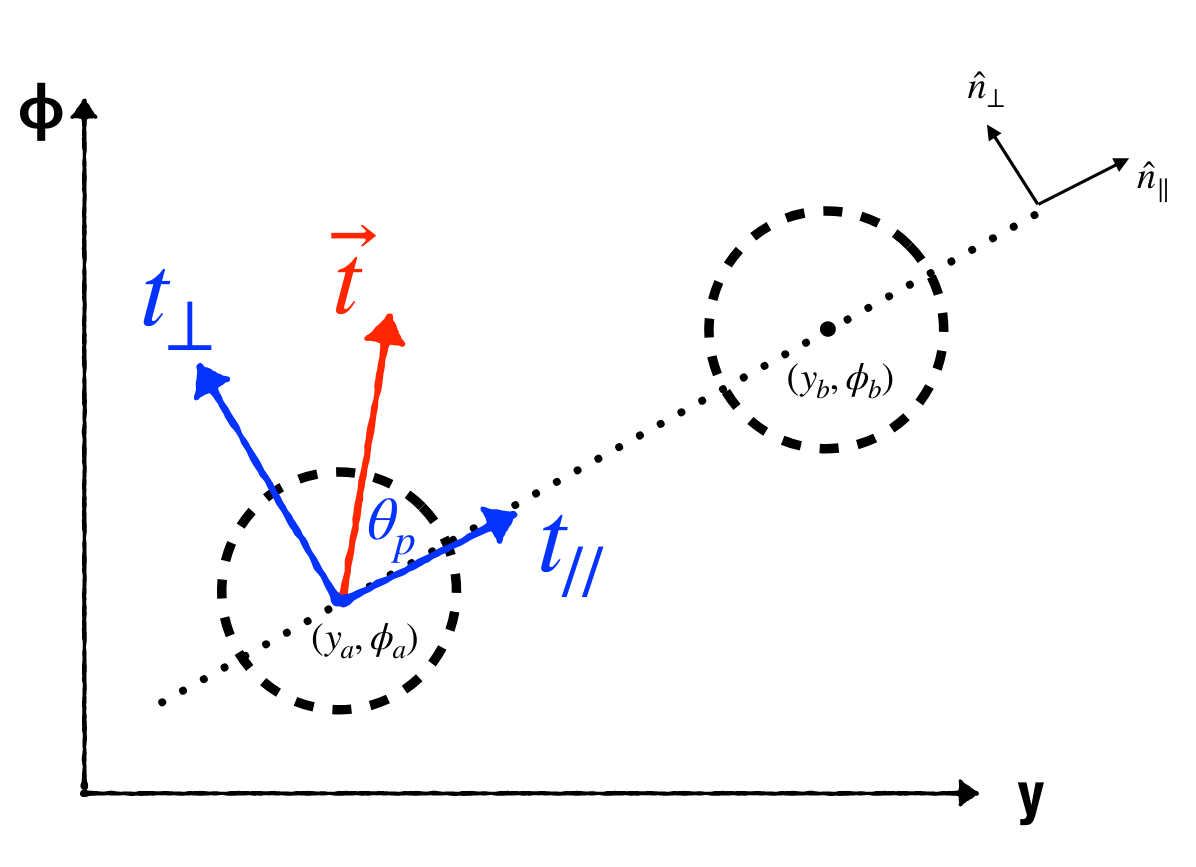
\includegraphics[scale=0.3]{ch4_images/pull_components}
\caption{The construction of the pull vector in the $(y, \phi)$ plane \cite{Larkoski:2019fsm}.}
\label{Pull vector}
\end{figure}
The pull vector $\vec{t}$ relative to jet $J_a$ is defined as
\begin{equation}
\vec{t} = \frac{1}{p_{ta}} \sum_{i \in J_a}p_{ti}\vert \vec{r}_i \vert^2 \hat{r}_i
\end{equation}
where $p_{t_a}$ is the transverse momentum of the jet, and the sum runs over all the the jet constituents. $y$ and $\phi$ again represent rapidity and azimuthal angle, and $\vec{r}_i$ is the distance vector between the jet and its $i$-th constituent in the $y$-$\phi$ plane
\begin{equation}
\vec{r}_i = (y_i - y_a, \phi_i - \phi_a).
\end{equation}
In particular, we would like to consider the projections of $\vec{t}$ along two lines: one, generated by the unit vector which points from the center of $J_a$ to the center of $J_b$ of the two jets
\begin{equation}
\hat{n}_\parallel = \frac{1}{\sqrt{\Delta y^2 + \Delta \phi^2}}\left(\Delta y, \Delta \phi \right),
\end{equation}
and the other generated by the unit vector perpendicular to $\hat{n}_\parallel$
\begin{equation}
\hat{n}_\perp = \frac{1}{\sqrt{\Delta y^2 + \Delta \phi^2}}\left(-\Delta \phi, \Delta y \right),
\end{equation}
i.e.
\begin{gather}
t_\parallel = \vec{t}\cdot \hat{n}_\parallel \\
t_\perp = \vec{t}\cdot \hat{n}_\perp
\end{gather}
We would also like to consider $\theta_{p}$, known as the pull angle, defined as
\begin{equation}
\theta_p = \arccos \frac{t_\parallel}{\vert \vec{t} \vert}.
\end{equation} 

The pull vector is sensitive to the different color connections which are present in the decay of a color singlet and the decay of a color octet.

 An illustration of this feature is shown in Figure \ref{color connections}. Because of the different color connections, the radiation from jets originating from a singlet decay will tend to be emitted between the two jets, causing the pull vector of $J_a$ to point in the direction of $J_b$ and vice-versa. In the octect case, the pull vectors will instead tend to point in different directions.
\begin{figure}[ht]
\centering
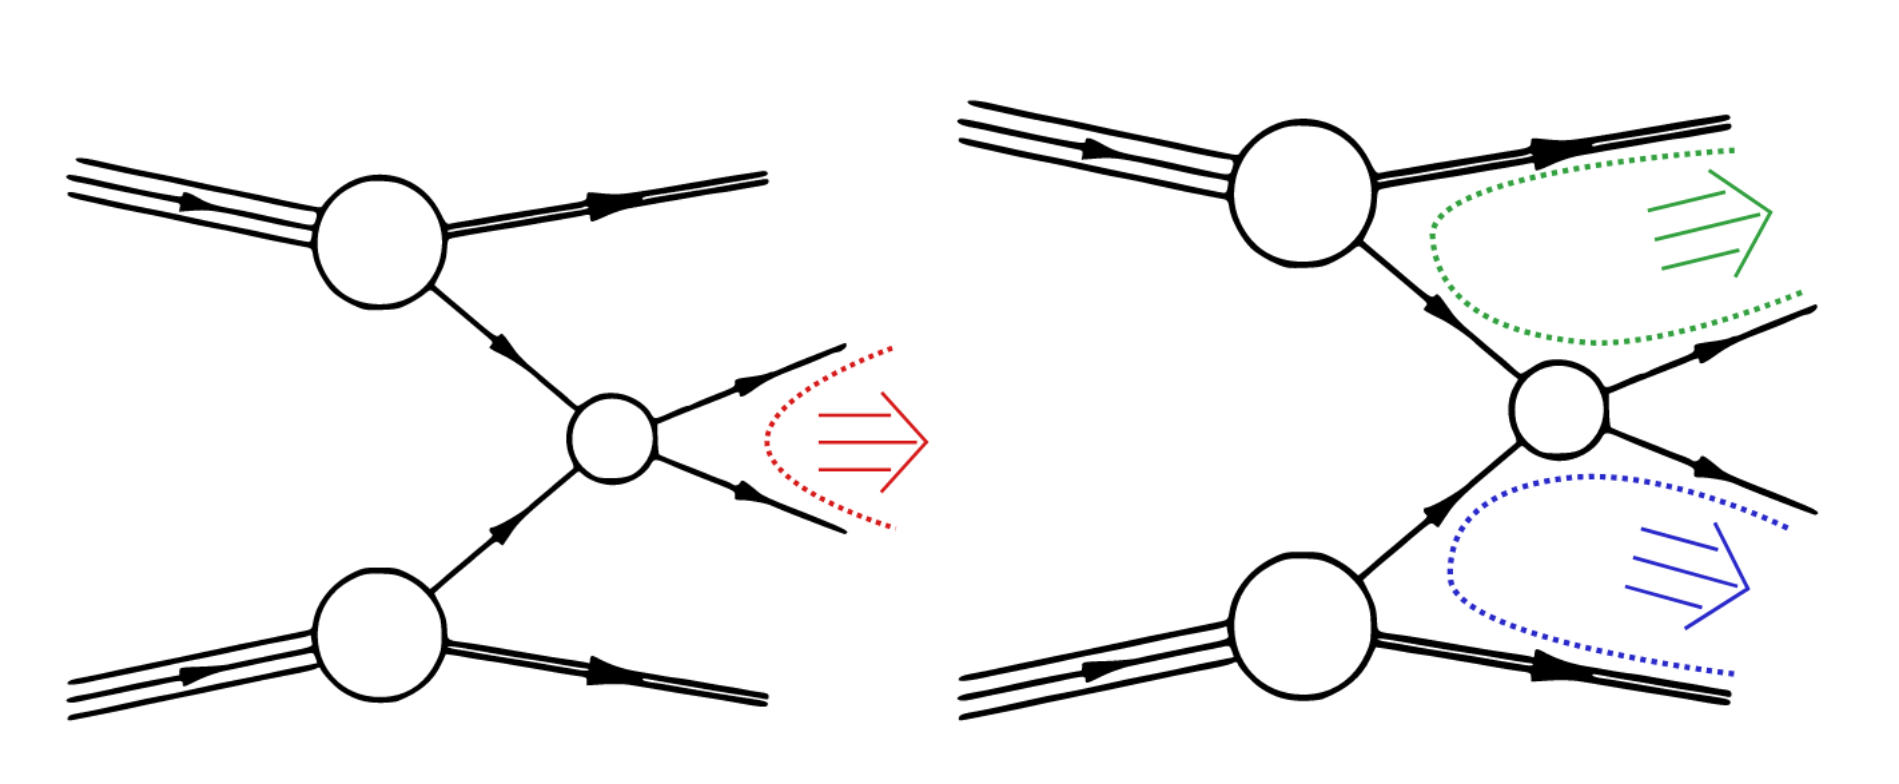
\includegraphics[scale=0.2]{ch4_images/color_configurations}
\caption{A representation of the color flow for the decay of a color singlet (left) vs. a color octect (right) at a collider experiment. In the case of a color singlet, the two colored particles stemming from the decay are color-connected only to each other, while for the case of an octect, the particles are color-connected to the rest of the proton, as it is from there that their color originates \cite{Gallicchio:2010sw}.}
\label{color connections}
\end{figure}


Of all the variables considered, the pull angle has been shown to be the most effective discriminator of the two different color configurations \cite{Gallicchio:2010sw}. However, there was a noticeable mismatch between theoretical predictions for $\theta_p$ and experimental measurements \cite{Larkoski:2019urm}. 

The theoretical difficulties in calculating $\theta_p$ stem from the fact that it is not an IRC safe variable. However, $t_\parallel$ and $t_\perp$ \emph{are} IRC safe observables. 

Our method includes these two variables for this purpose. $\theta_p$ is also included since it can be measured at experiments, and its discrimination potential is still good. We consider these variables for both jets $J_a$ and $J_b$. 

\subsection{$D_2$}

To introduce the observable $D_2$, we must first familiarize the reader with energy correlator functions (ECF) \cite{Larkoski:2013eya}. These are a class of observables sensitive to jet substructure. Specifically, they are sensitive to a the number of prongs of a jet, or how many distinct subjets compose a given jet. This is particularly useful in the boosted regime, defined by $p_T \gg 1$, where kinematics forces jets, which would otherwise be separated, to come together, as shown in Figure \ref{two pronged boost}. The $(N+1)$-point correlator is used to determine if a jet has $N$ prongs.

\begin{figure}[ht]
\centering
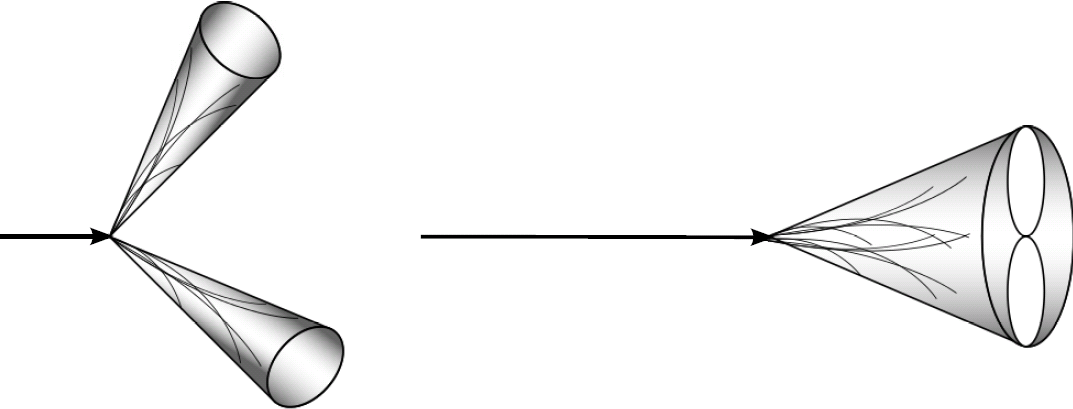
\includegraphics[scale=0.35]{ch4_images/two_prong}
\caption{An illustration of a 2-prong jet caused by boosted kinematics \cite{jet_image}.}
\label{two pronged boost}
\end{figure}

The definition of the $N$-point ECF is based on the  the $p_T$ and angular distance between the components of a jet:
\begin{equation}
ECF(N,\beta) = \sum_{i_1 < i_2 < \dots < i_N \in J} \left( \prod_{a = 1}^N p_{Ti_a} \right) \left(\prod_{b = 1}^{N-1} \prod_{c = b + 1}^N  R_{i_b i_c}\right)^\beta,
\label{ECF definition}
\end{equation}
where $\beta$ is an arbitrary parameter. If $\beta > 0$, the observable is IRC safe. 
For the sake of clarity, let us write out the first few ECFs:
\begin{gather*}
ECF(0, \beta) = 1\\
ECF(1, \beta) = \sum_{i\in J}p_{Ti} \\
ECF(2, \beta) = \sum_{i < j \in J} p_{Ti}p_{Tj} R_{ij}^\beta \\
ECF(3, \beta) = \sum_{i < j < k \in J} p_{Ti}p_{Tj}p_{Tk} \left(R_{ij}R_{ik}R_{jk}\right)^\beta.
\end{gather*}
There exists also a normalized $N$-point ECF, $e^{(\beta)}_N$, which differs from the definition (\ref{ECF definition}) by a factor proportional to the $p_T$ of the jet
\begin{equation}
e^{(\beta)}_N = \left(\frac{1}{p_{TJ}}\right)^N ECF(N,\beta)
\end{equation}

Clearly, $ECF(N,\beta) = 0$ when it is computed on a jet with fewer than $N$ constituents. In addition to this, $ECF(N+1, \beta)$ will be significantly smaller than $ECF(N,\beta)$ if calculated on a jet containing only $N$ subjets. This naturally leads to the consideration of the following ratio:
\begin{equation}
r_N^\beta = \frac{ECF(N+1,\beta)}{ECF(N,\beta)}.
\end{equation}
The ratio $r_N^\beta$ is useful to discriminate $N$-prong jets from $N+1$-prong jets. The $D_2$ variable \cite{Larkoski:2014gra} is a variation on this ratio, specified to the case of 1-prong and 2-prong jets, and calculated using the normalized ECFs
\begin{equation}
D_2(\beta) = \frac{e^{(\beta)}_3}{(e^{(\beta)}_2)^3}
\end{equation}
Due to the different color configurations, a large jet originating from the decay of a color singlet in the boosted regime will tend to exhibit a 2-prong substructure, and thus will tend to have a larger value of $D_2$. On the other hand, in the case of a color octect, the same decay will tend to have a 1-prong structure, leading to smaller values for the observable.

For the purpose of our study, we have chosen the value $\beta = 2$.

\subsection{Color Ring}
The final variable we have considered is known as the \emph{color ring}. To derive the observable, we must consider the boosted decay of a color singlet into two jets, which, at the parton level, correspond to (anti)quarks or gluons. We will consider the decay into two hard partons and the subsequent emission of a low-energy gluon.

The matrix element describing this transition is as follows \cite{Buckley:2020kdp}:
\begin{equation}
\vert \mathcal{M}_S \vert^2 = -\mathbf{T}_\alpha \cdot \mathbf{T}_\beta 	\frac{n_a \cdot n_b}{(n_a \cdot k)(n_b \cdot k)}.
\end{equation}
In this expression, $n_a$ and $n_b$ are the light-like vectors parallel to the hard jets, $k$ is the impulse of the soft emission, and $\mathbf{T}_i$ is the color operator. The dependence on $\alpha_S$ has been neglected as it is not relevant at this level. In what follows, Latin indices are used to refer to kinematics while Greek indices refer to color.

We know that color must be conserved, and since we are dealing with a singlet decay, we must have
\begin{equation}
\mathbf{T}_\alpha + \mathbf{T}_\beta = 0.
\end{equation}
This necessarily implies that $\beta = \overline{\alpha}$, and so
\begin{equation}
-\mathbf{T}_\alpha \cdot \mathbf{T}_\beta = \mathbf{T}_\alpha^2 = C_S\mathbf{1}
\end{equation}
where $C_S$ is Casimir operator for either the fundamental or adjoint representation of $SU(3)$, depending on the decay, and we have explicitly written the identity matrix. 

Let us now consider the same matrix element for a background process, in which a color octect decays into two hard partons, with a subsequent soft emission in the boosted regime. Thanks to the boosted kinematics of the event, we can safely assume that the two hard partons are closer in angle to each other than to any other colored object, allowing for the factorization of the matrix element into two elements. The first describes the dipole formed by the hard partons and the emission of the soft radiation. The second contains additional contributions from the initial state of the event and from extra jets, if present. This term will again be neglected since it will lead to a constant. We can thus write
\begin{equation}
\vert \mathcal{M}_B \vert^2 = \sum_{\alpha, \beta} \left[ -\mathbf{T}_\alpha \cdot \mathbf{T}_\beta 	\frac{n_a \cdot n_b}{(n_a \cdot k)(n_b \cdot k)} - \mathbf{T}_\alpha \cdot \mathbf{T}_\gamma \frac{n_a \cdot \overline{n}}{(n_a \cdot k)(\overline{n} \cdot k)} - \mathbf{T}_\beta \cdot \mathbf{T}_\gamma 	\frac{n_b \cdot \overline{n}}{(n_b \cdot k)(\overline{n} \cdot k)} \right]
\label{bkg matrix element}
\end{equation}
where $\overline{n}$ is a light-like vector antiparallel to the system. $\overline{n}$ has overall color $\gamma$ which is fixed by the relation
\begin{equation}
\mathbf{T}_\alpha + \mathbf{T}_\beta + \mathbf{T}_\gamma = 0.
\end{equation}
We can use this to simplify the expression (\ref{bkg matrix element}), which becomes
\begin{equation}
\vert \mathcal{M}_B \vert^2 = \sum_{\alpha, \beta} \left[ -\mathbf{T}_\alpha \cdot \mathbf{T}_\beta 	\frac{n_a \cdot n_b}{(n_a \cdot k)(n_b \cdot k)} + (\mathbf{T}_\alpha^2 + \mathbf{T}_\alpha \cdot \mathbf{T}_\beta)\left(\frac{n_a \cdot \overline{n}}{(n_a \cdot k)(\overline{n} \cdot k)} + \frac{n_b \cdot \overline{n}}{(n_b \cdot k)(\overline{n} \cdot k)}\right) \right].
\end{equation}
The background matrix element has been written in terms of two color factors:
\begin{equation}
\begin{cases}
C_B = -\mathbf{T}_\alpha \cdot \mathbf{T}_\beta \\
\tilde{C}_B = \mathbf{T}_\alpha^2 + \mathbf{T}_\alpha \cdot \mathbf{T}_\beta.
\end{cases}
\end{equation}
Again, the exact color factor depends on the process considered. We are interested in $H\rightarrow b\overline{b}$ as our signal process, which fixes $C_S = C_F$ and $C_B = C_F - C_A/2$ and $\widetilde{C}_B = C_A/2$. A decay into gluons, e.g. $H\rightarrow gg$ would fix these constants differently.

It is a well-established fact that the optimal variable to discriminate these two configurations is monotonic in their ratio \cite{Neyman1992}. The ratio turns out to be
\begin{equation}
\frac{\vert \mathcal{M}_S \vert^2}{\vert \mathcal{M}_B \vert^2} \simeq \frac{(n_a \cdot \overline{n})(n_b \cdot k)}{(n_a \cdot n_b)(\overline{n} \cdot k)} + \frac{(n_b \cdot \overline{n})(n_a \cdot k)}{(n_a \cdot n_b)(\overline{n} \cdot k)}
\end{equation}
where we have left out the color factors as they are just constants. If we assume the collinear limit and utilize the small-angle approximation, this expression simplifies to 
\begin{equation}
\frac{\vert \mathcal{M}_S \vert^2}{\vert \mathcal{M}_B \vert^2} \simeq \frac{\theta_{ak}^2 + \theta_{bk}^2}{\theta_{ab}^2} \equiv \mathcal{O}.
\label{color ring}
\end{equation}
$\mathcal{O}$ is the definition of the jet color ring. This variable gets its name from its geometric interpretation, shown in Figure \ref{color ring geometry}. Radiation from color singlets will tend to fall between the two jets, leading to values of $\mathcal{O} < 1$, while in the case of color octects, we will tend to have $\mathcal{O} > 1$. 
\begin{figure}
\centering
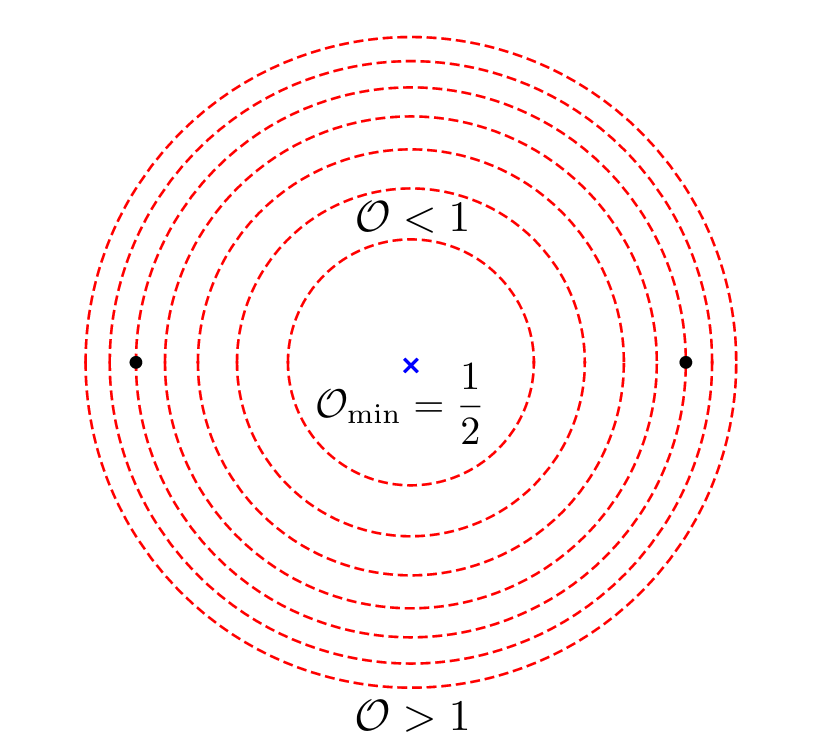
\includegraphics[scale=0.3]{ch4_images/cr}
\caption{A geometric interpretation of the color ring. The two black dots represent the two hard jets, and the contour passing through them has value $\mathcal{O} = 1$. Depending on the direction of $k$, the $\mathcal{O}$ can assume different values. If $k$ is collinear to either $a$ or $b$, $\mathcal{O}$ assumes its minimum value \cite{Buckley:2020kdp}.}
\label{color ring geometry}
\end{figure}

Unfortunately, without any sort of momentum-weighting, (\ref{color ring}) cannot be IRC safe. However, if we assume that the emission of the soft gluon leads to a distinct subjet within a larger jet, then IRC safety is recovered.

\section{Simulation}
\label{Simulation}

The aforementioned variables are implemented using information from event creation via Monte Carlo simulation. Using \code{MadGraph5\_aMC} v2.8.3.2 \cite{Alwall:2014hca}, we generated two hard processes:
\begin{gather}
p p \rightarrow Z(\nu_\ell \overline{\nu}_\ell) H(b\overline{b}) \\
p p \rightarrow b\overline{b} \nu_\ell \overline{\nu}_\ell.
\end{gather}

The first process, hereby referred to as the \emph{signal}, represents the most likely decay of the Higgs, a color singlet. The second process, or the \emph{background}, contains all QCD diagrams which lead to the same final state as the signal. Figure \ref{zhbb + gbb feynman diagrams} shows the Feynman diagrams constituting the signal and the background. Both processes were generated with a 200 GeV cut on the $p_T$ of the neutrino pair in the final state. This was done to ensure that the events generated were firmly in the boosted regime. The outputs of the parton-level simulations were saved as Les Houches Event Files \cite{Alwall:2006yp}.

\begin{figure}
\begin{subfigure}{.5\textwidth}
\centering
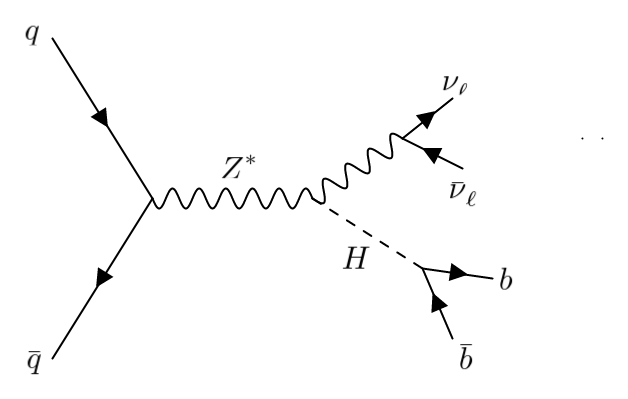
\includegraphics[scale=0.6]{ch4_images/zhbb}
\caption{}
\end{subfigure}
\begin{subfigure}{.5\textwidth}
\centering
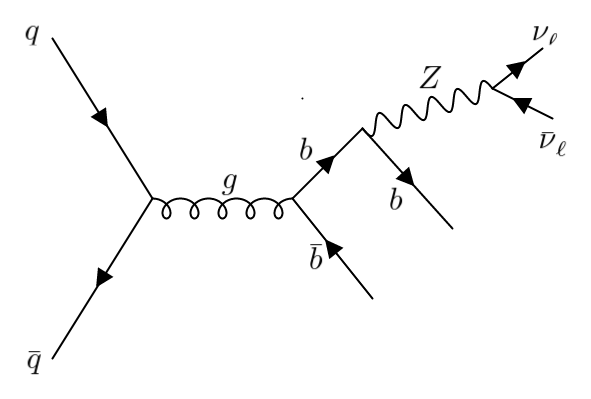
\includegraphics[scale=0.15]{ch4_images/gbb1}
\caption{}
\end{subfigure}
\begin{subfigure}{.5\textwidth}
\centering
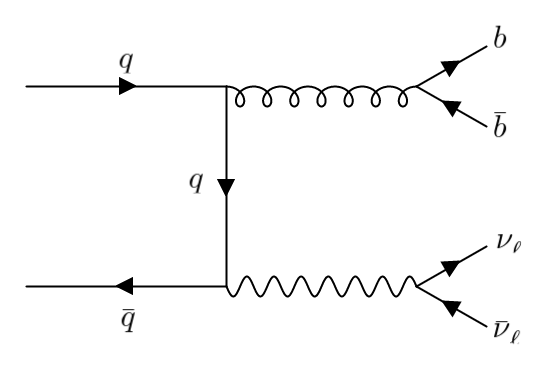
\includegraphics[scale=0.15]{ch4_images/gbb2}
\caption{}
\end{subfigure}
\begin{subfigure}{.5\textwidth}
\centering
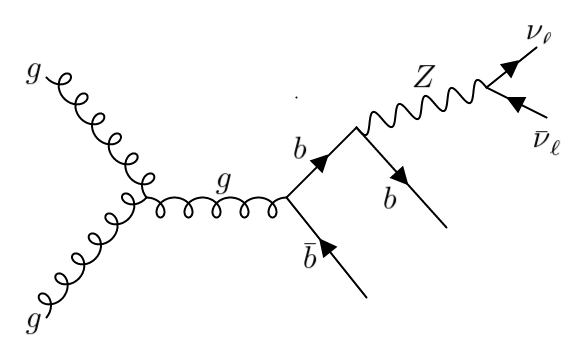
\includegraphics[scale=0.15]{ch4_images/gbb3}
\caption{}
\end{subfigure}
\caption{The Feynman diagrams constituting the signal (a) and background (b),(c),(d). \todo{mettere immagine migliore}.}
\label{zhbb + gbb feynman diagrams}
\end{figure}

These hard processes were subsequently showered in \code{PYTHIA8} v8.305 \cite{Sjostrand:2014zea}. This program simulates the perturbative evolution of the event (e.g. radiation) as well as hadronization to produce particle-level events. The simulation included both Multi Parton Interactions and underlying events. The output of the \code{PYTHIA8} shower was saved as a \code{HepMC3} file \cite{BUCKLEY2021107310, Dobbs:2001ck}. \code{HepMC3} v3.2.2 was used.

Finally, rather than simulating an entire detector, \code{DELPHES} v3.5.0 was used to perform a fast detector simulation \cite{Ovyn:2009tx, deFavereau:2013fsa}. This allowed us to understand how our method would perform in reality without having to run a computationally expensive full simulation, which in addition is strongly detector dependent. From \code{DELPHES}, we extracted both the Monte Carlo truth of the event, containing the particle level information, as well as the reconstructed events including the \code{DELPHES}-smeared detector effects. 

The \code{DELPHES} simulation was run using a version of the ATLAS card modified to fit our analysis standards. The output was stored as a \code{ROOT} file, and \code{ROOT} v6.22/06 was used \cite{fons_rademakers_2020_3895852}. 

In total, we simulated 1M signal and background events.


\section{Analysis}

We analyzed the simulated data in both the truth case and the reconstructed case. These cases differ in just one aspect: for the truth case, all stable particles with $p_T > 0.5$ GeV were clustered into jets. In the reconstructed case, the jets were clustered using the simulated calorimeter towers and tracks. All electromagnetic calorimeter towers with energy $E > 0.5$ GeV and significance $S > 2.0$ and all hadronic calorimeter towers with energy $E > 1.0$ GeV and significance $S > 2.0$ are considered. Tracks are required to have $p_T > 0.5$ GeV. The jets are clustered using \code{FastJet} v3.3.4 \cite{Cacciari:2011ma}.

We can now discuss the details of the analysis. First, the constituents are clustered into Large Jets with radius $R=1.0$.  For  each  event,  we  choose  the jet with the highest $p_T$ as the Large Jet. We only accept the event if the jet has $p_T > 250$ GeV, $\vert y \vert < 1.5$, and invariant mass $m_J \in [0,500]$ GeV. The restriction on $y$ comes from experimental considerations: due to limitations related to the detector acceptance, b-tagging outside of this region comes with large errors. 

We  also  cluster  the  constituents  into  smaller  jets with radius $R = 0.2$. We identify those jets which distance $\Delta R < 0.8$ from the selected Large Jet, and call these subjets. We then proceed to identify the b-subjets which originate from the b-partons, through a process known as \emph{b-labelling}. We do this by first identifying the b-partons originating from the hard scattering in the event record. For each b-parton, we find the closest subjet. If the b-parton has $p_T > 5.0$ GeV and the subjet is within $\Delta R = 0.2$ from the b-parton, we label the subjet as a b-subjet. 

For the event to be accepted, we require that there be two unique b-labelled subjets with $p_T > 10$ GeV. The pull variables are calculated on these two b-labelled subjets, and $D_2$ is calculated on the Large Jet. For the color ring to be defined, there must also be a third non-b subjet within $\Delta R = 0.8$ from the Large Jet. In a majority of cases, this third jet is not present. To avoid discarding too many events, in these cases we assign a default value of $\mathcal{O} = -1$ to the color ring. This allows for higher statistics, but also provides useful information to the machine learning algorithms.

Table \ref{Efficiencies table} shows the percentage of events which passed the selections in all cases considered. The cuts were more severe on the background events than the signal events in both the truth and reconstructed cases. Two cuts are significantly more important than the rest: the $p_T$ cut on the Large Jet, responsible for about 60\% of all cuts, and the rapidity cut on the Large Jet, responsible for another 10\%.

\begin{table}[!htb]
    \begin{minipage}{.5\linewidth}
      %\caption{}
      \centering
        \begin{tabular}{|c|c|}
		\hline 
		\multicolumn{2}{|c|}{\textbf{Truth}} \\ 
		\hline 
		\* & Events Passed \\ 
		\hline 
		Signal & 20\% \\ 
		\hline 
		Background & 1.6\% \\ 
		\hline 
		\end{tabular}  
    \end{minipage}%
    \begin{minipage}{.5\linewidth}
      \centering
        %\caption{}
        \begin{tabular}{|c|c|}
		\hline 
		\multicolumn{2}{|c|}{\textbf{Reco}} \\ 
		\hline 
		\* & Events Passed \\ 
		\hline 
		Signal & 17\% \\ 
		\hline 
		Background & 1.3\% \\ 
		\hline 
		\end{tabular} 
    \end{minipage} 
    \caption{The approximate efficiencies of the analysis after all cuts were applied.}
    \label{Efficiencies table}
\end{table}

Figure \ref{sgn/bkg true} shows the distributions of the 8 variables for the truth case. In Figure \ref{sgn/bkg reco}, the same distributions are shown in the reconstructed case. In both cases, clear differences between signal and background allow for discrimination of the two.

\begin{figure}
\captionsetup[subfigure]{labelformat=empty}
\begin{subfigure}{.33\textwidth}
\centering
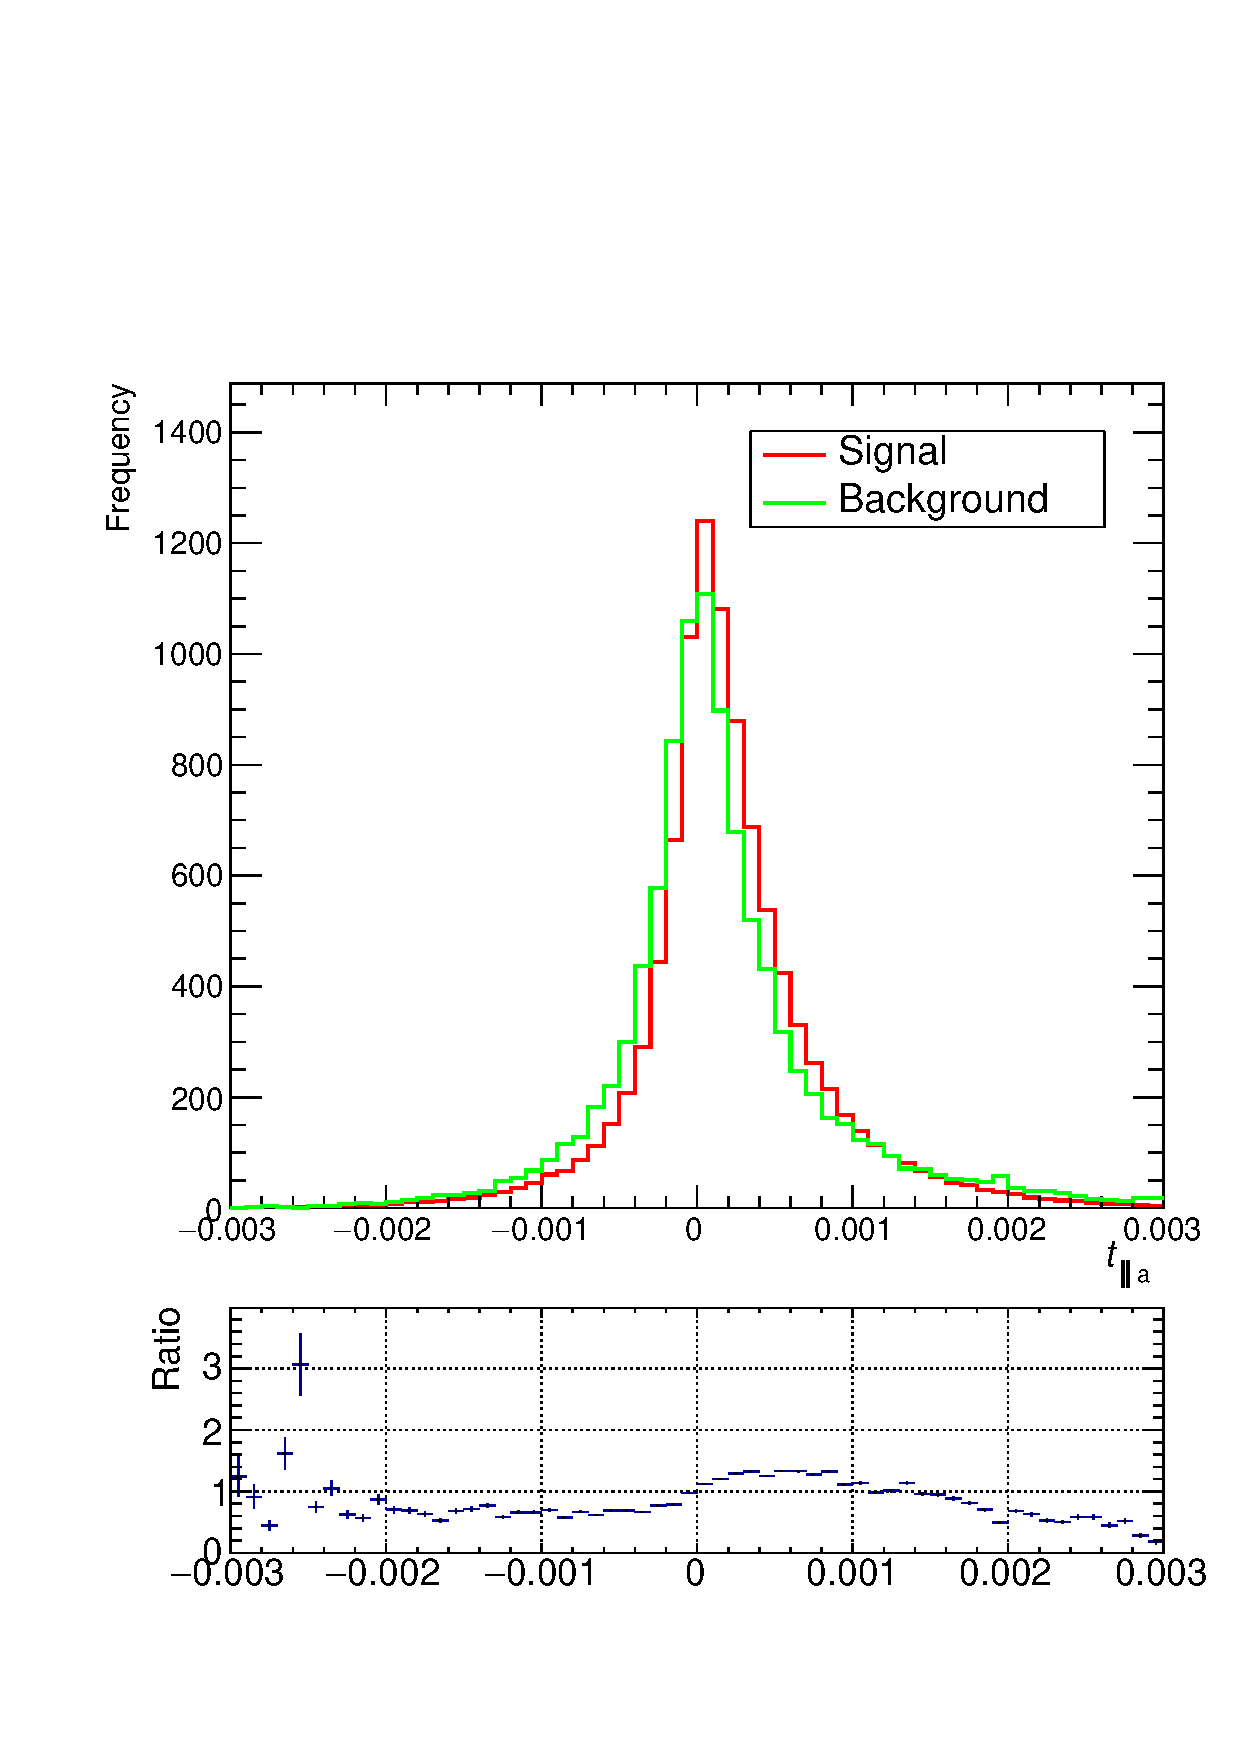
\includegraphics[scale=0.25]{truth/tpar1}
\caption{$t_{\parallel a}$}
\end{subfigure}
\begin{subfigure}{0.33\textwidth}
\centering
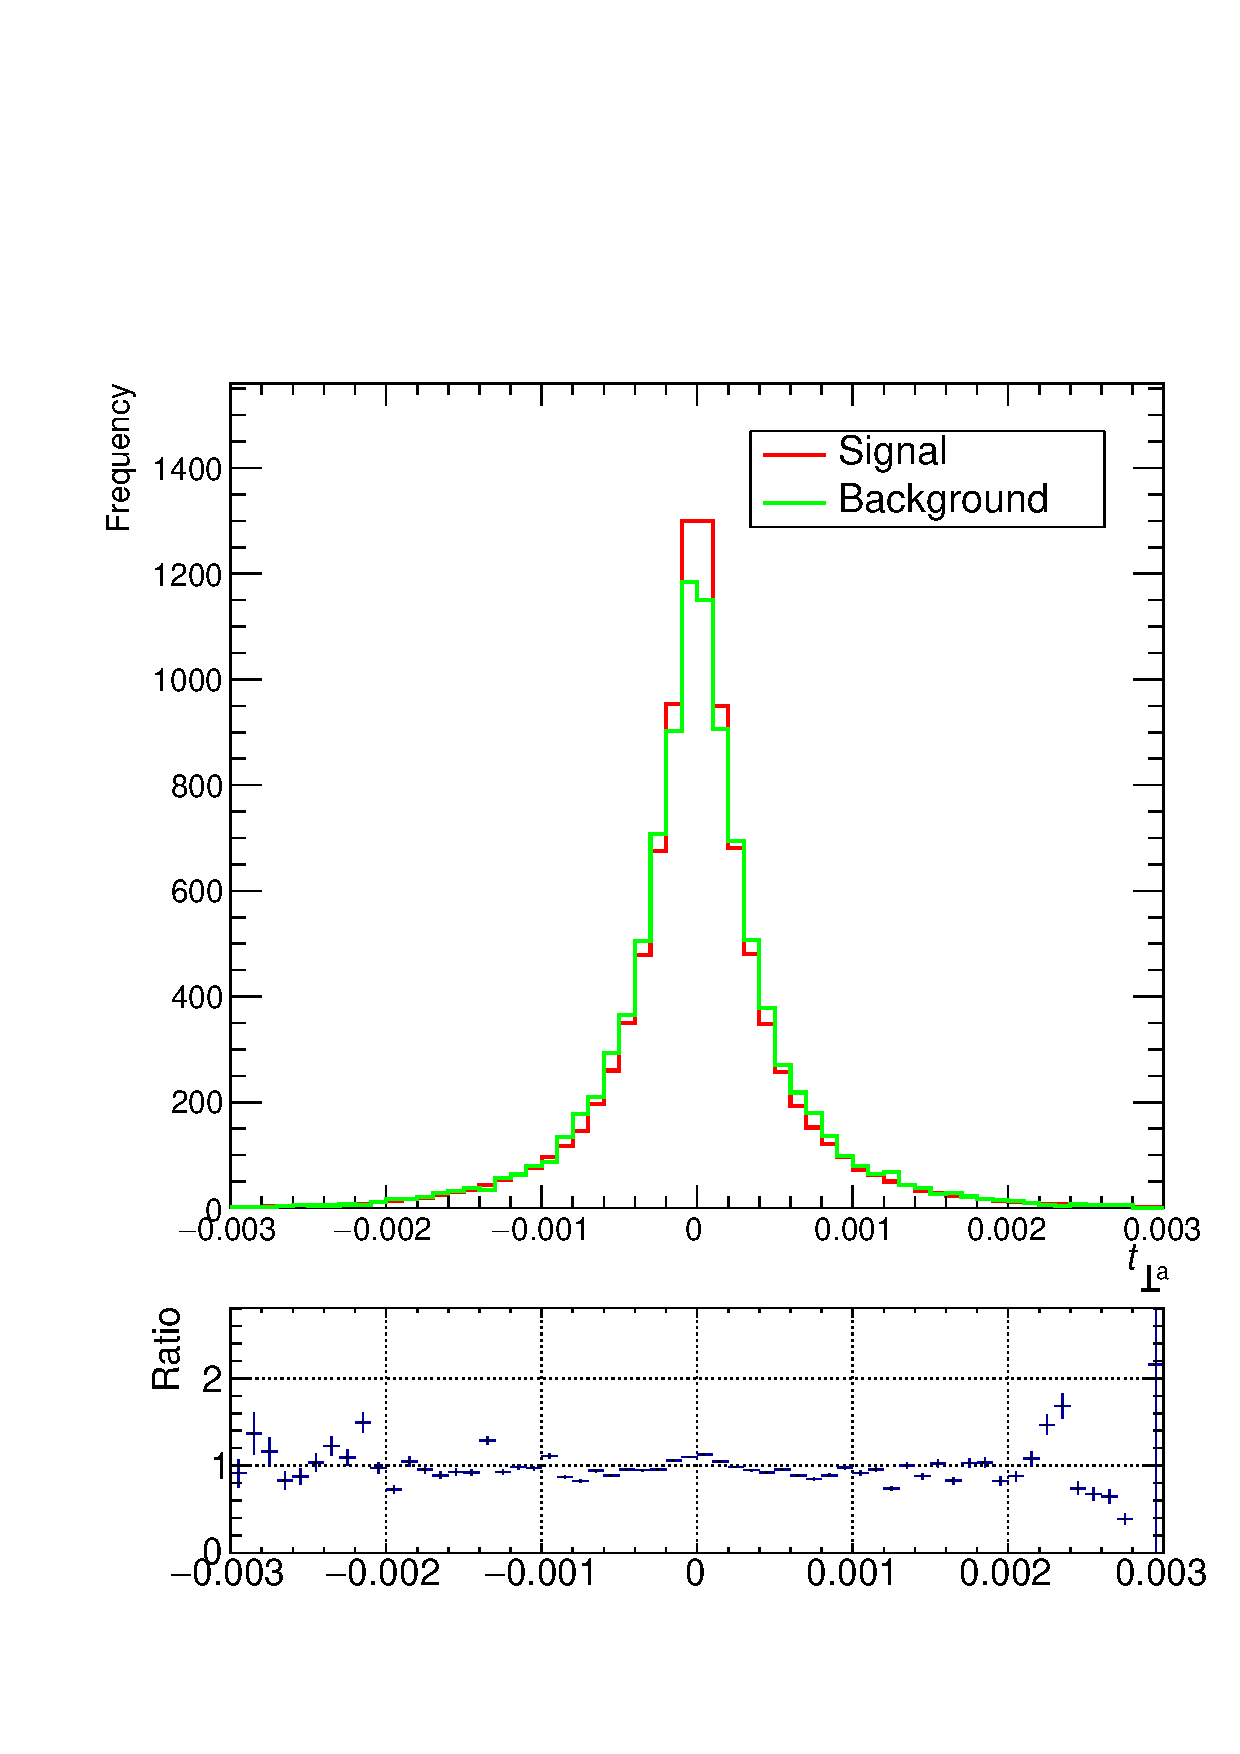
\includegraphics[scale=0.25]{truth/tper1}
\caption{$t_{\perp a}$}
\end{subfigure}
\begin{subfigure}{.33\textwidth}
\centering
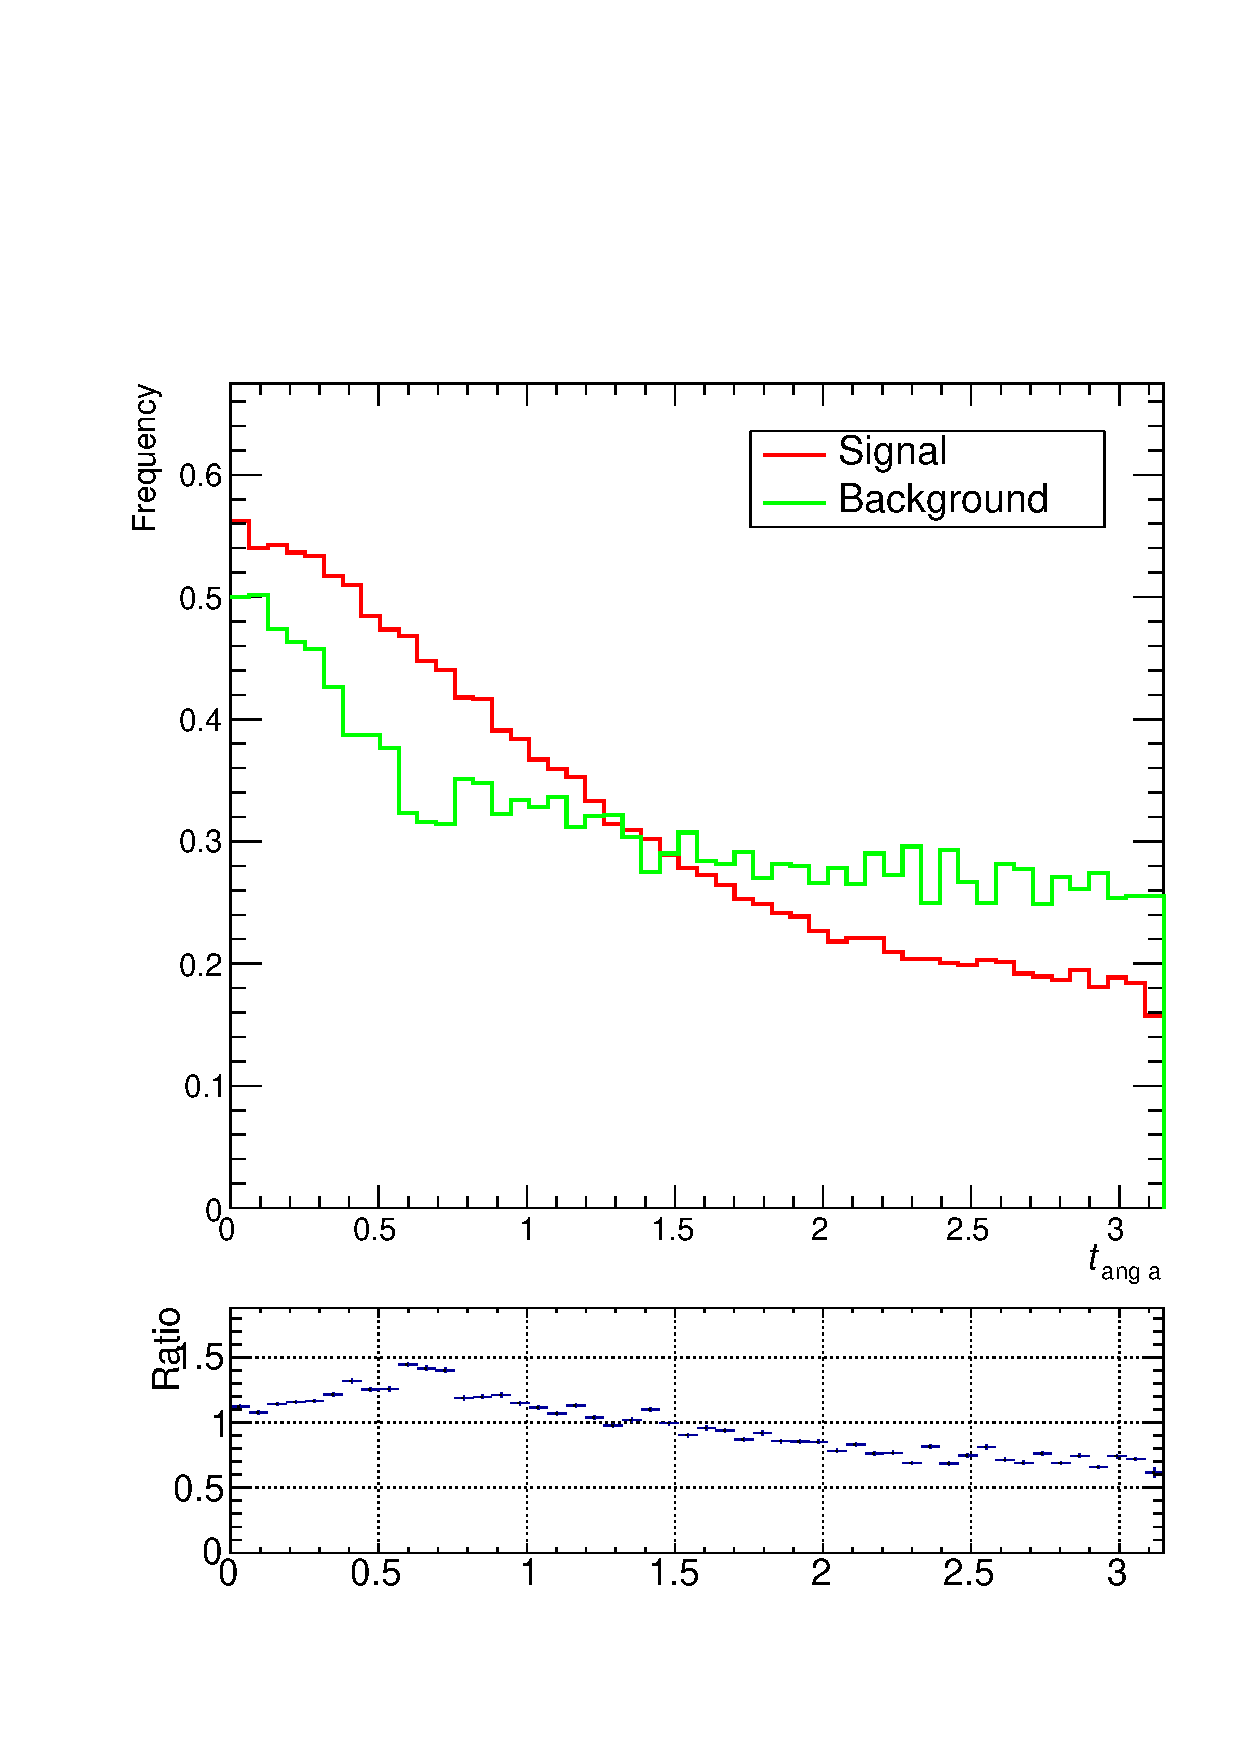
\includegraphics[scale=0.25]{truth/tang1}
\caption{$\theta_{pa}$}
\end{subfigure}
\begin{subfigure}{.33\textwidth}
\centering
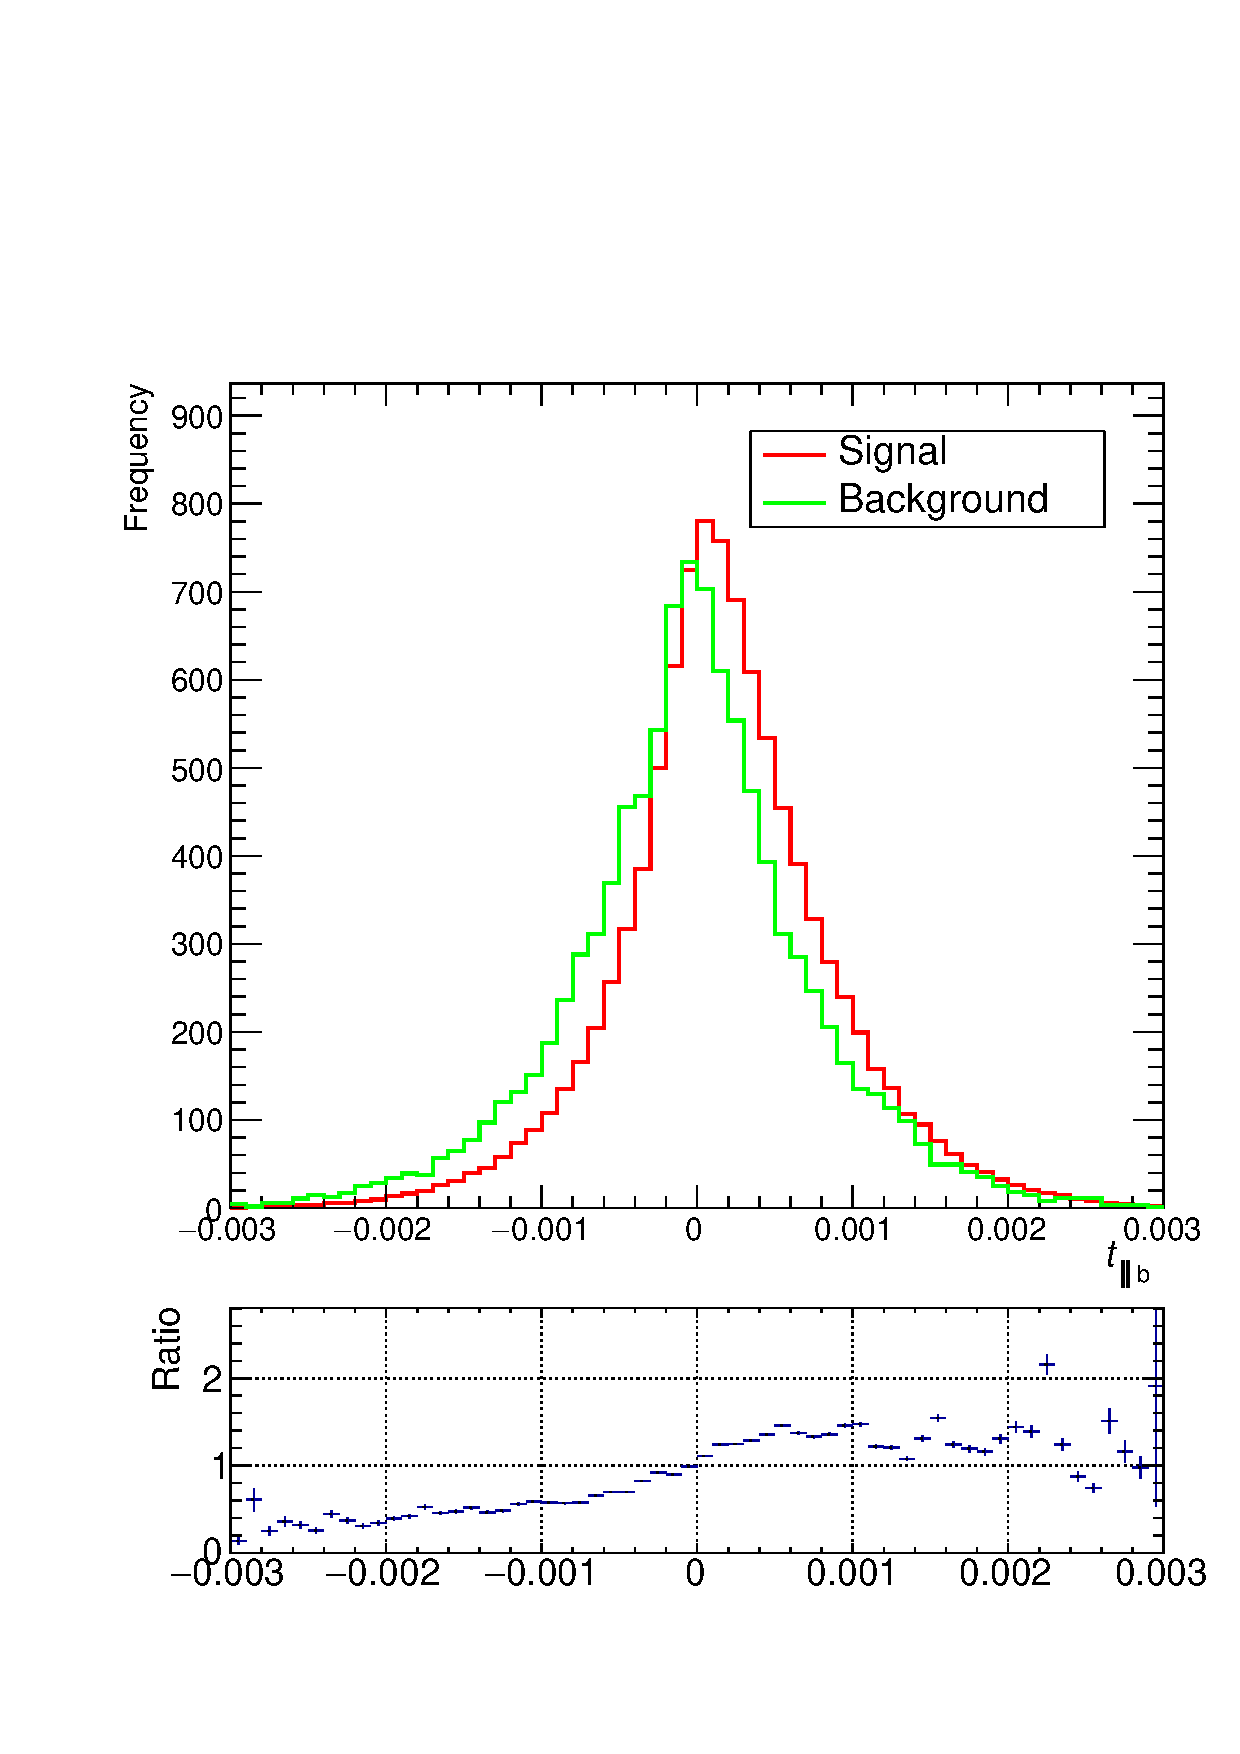
\includegraphics[scale=0.25]{truth/tpar2}
\caption{$t_{\parallel b}$}
\end{subfigure}
\begin{subfigure}{0.33\textwidth}
\centering
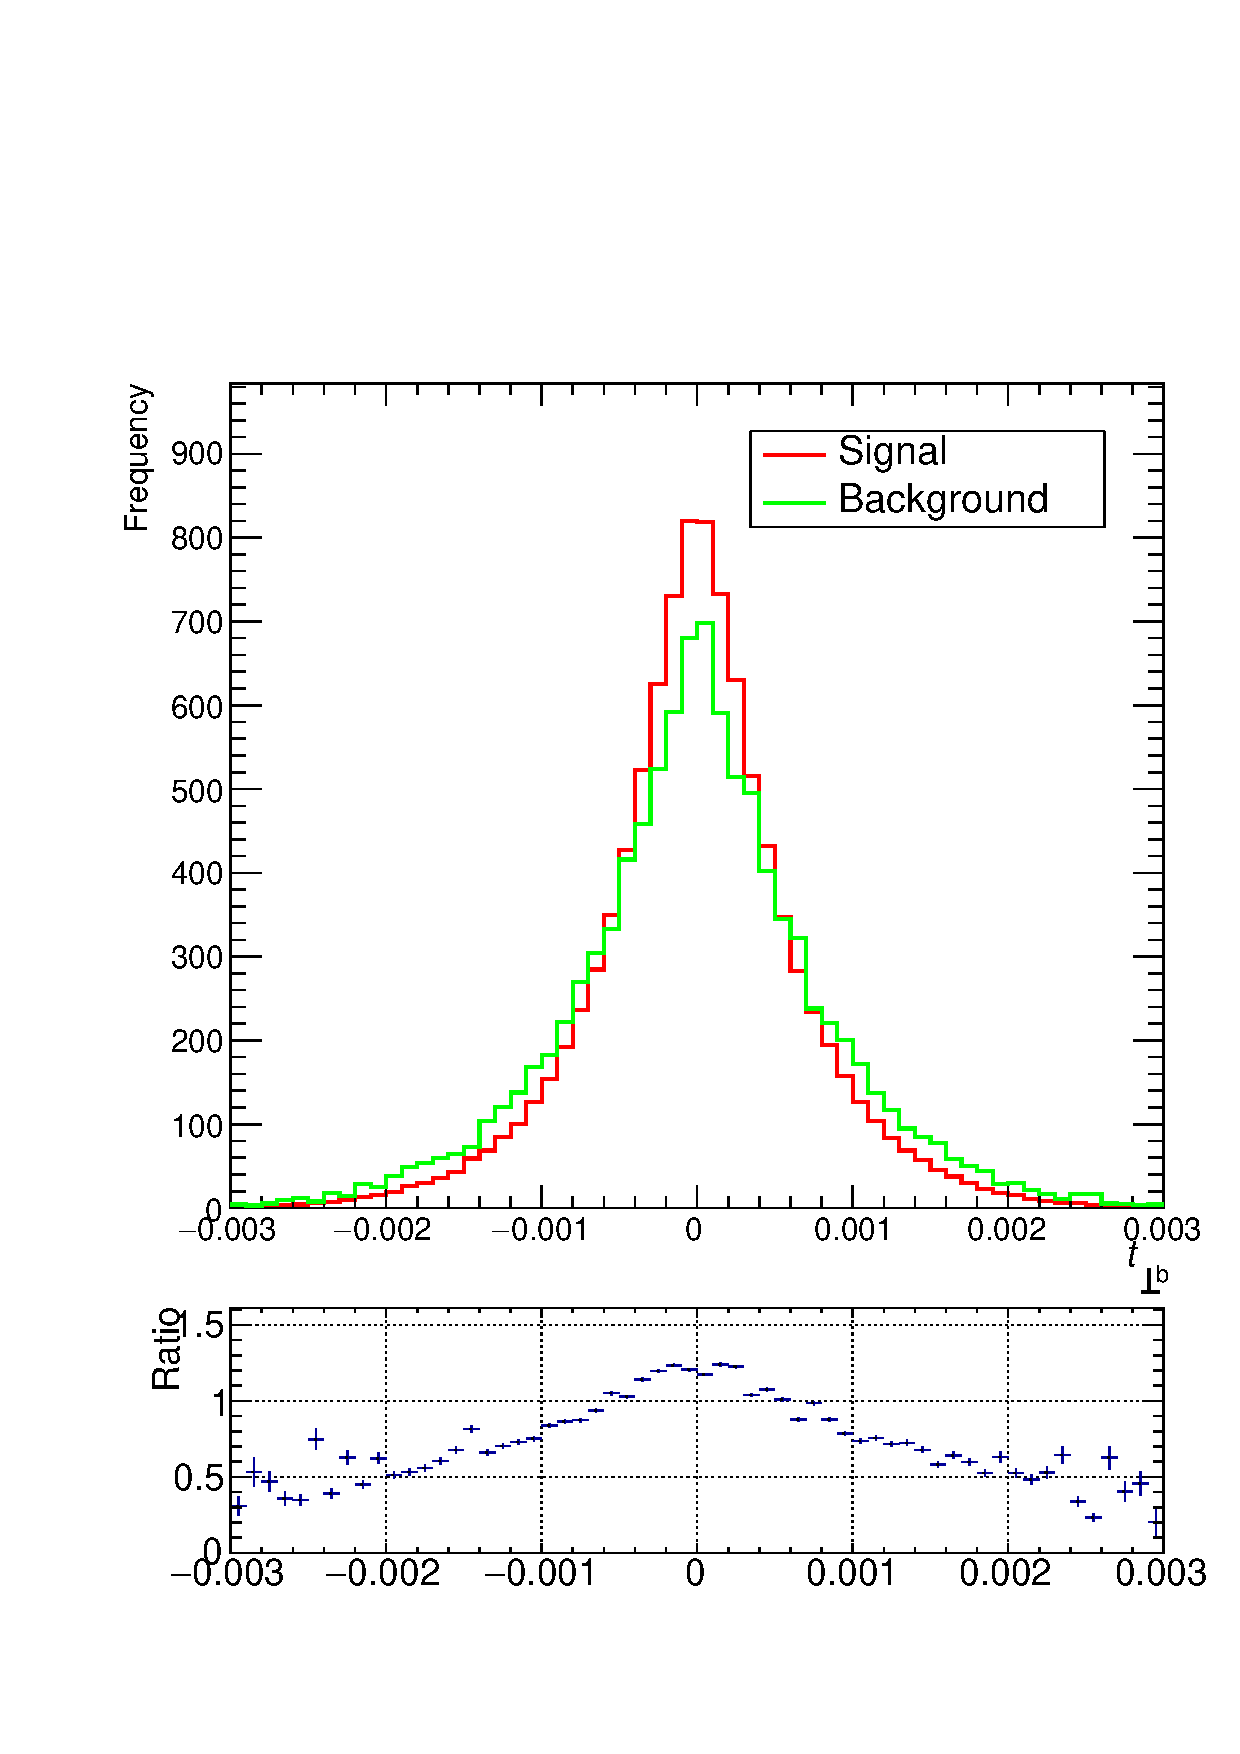
\includegraphics[scale=0.25]{truth/tper2}
\caption{$t_{\perp b}$}
\end{subfigure}
\begin{subfigure}{.33\textwidth}
\centering
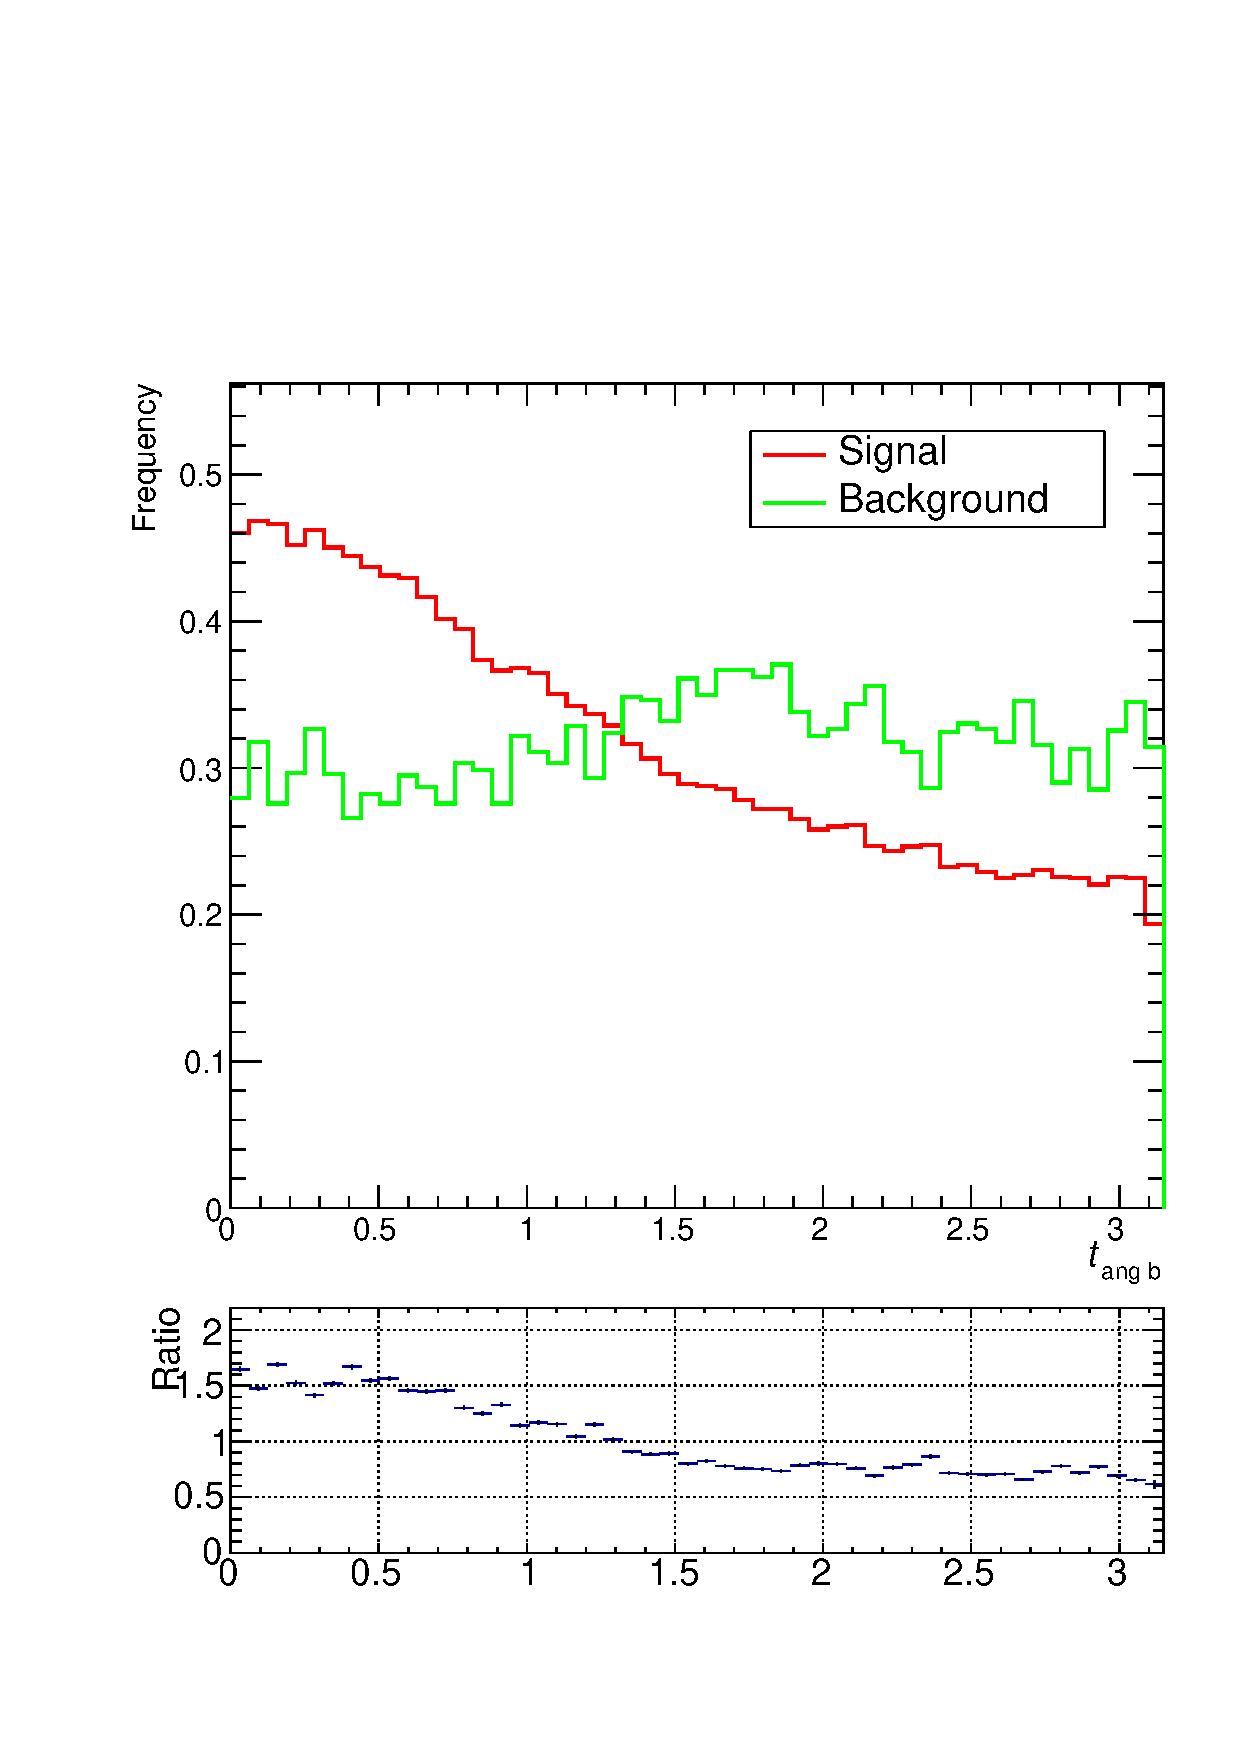
\includegraphics[scale=0.25]{truth/tang2}
\caption{$\theta_{pb}$}
\end{subfigure}
\begin{subfigure}{0.5\textwidth}
\centering
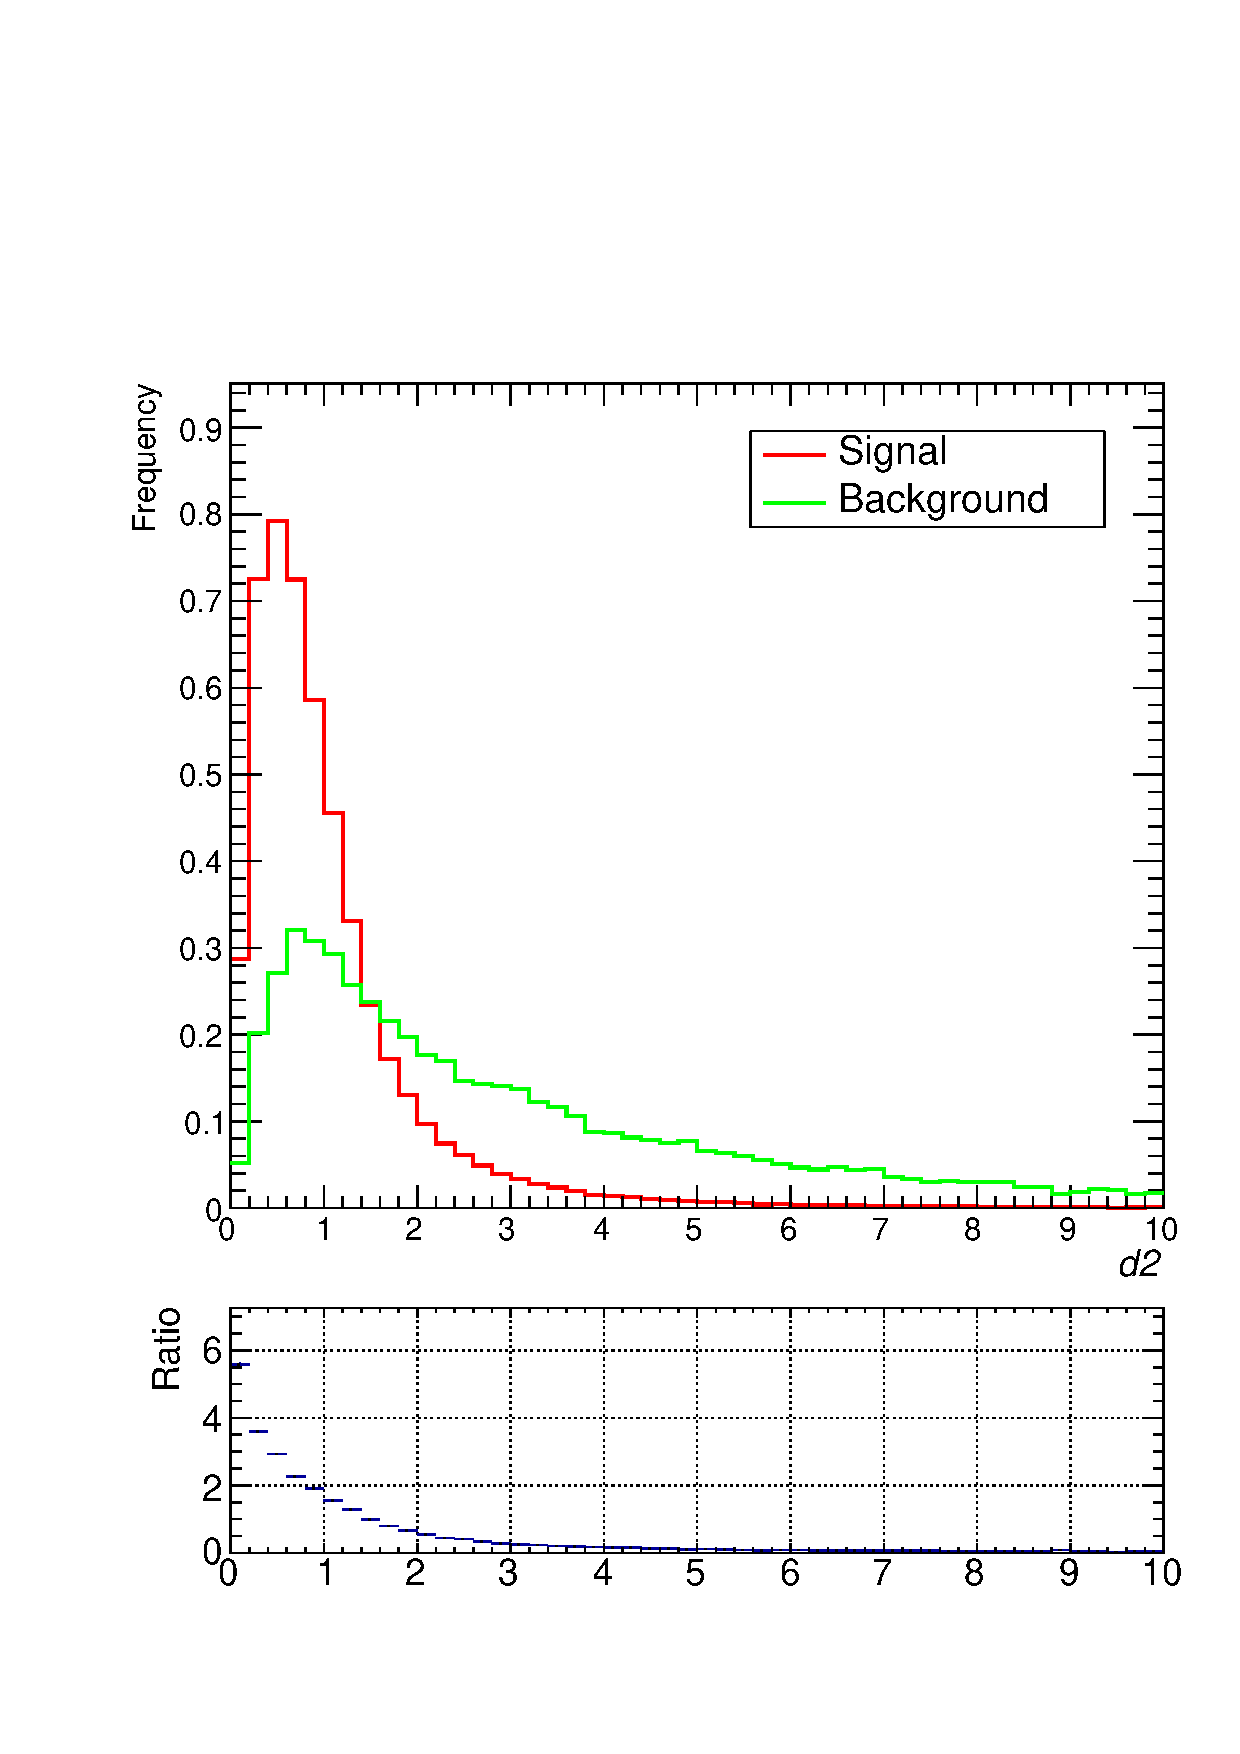
\includegraphics[scale=0.25]{truth/d2}
\caption{$D_2$}
\end{subfigure}
\begin{subfigure}{.5\textwidth}
\centering
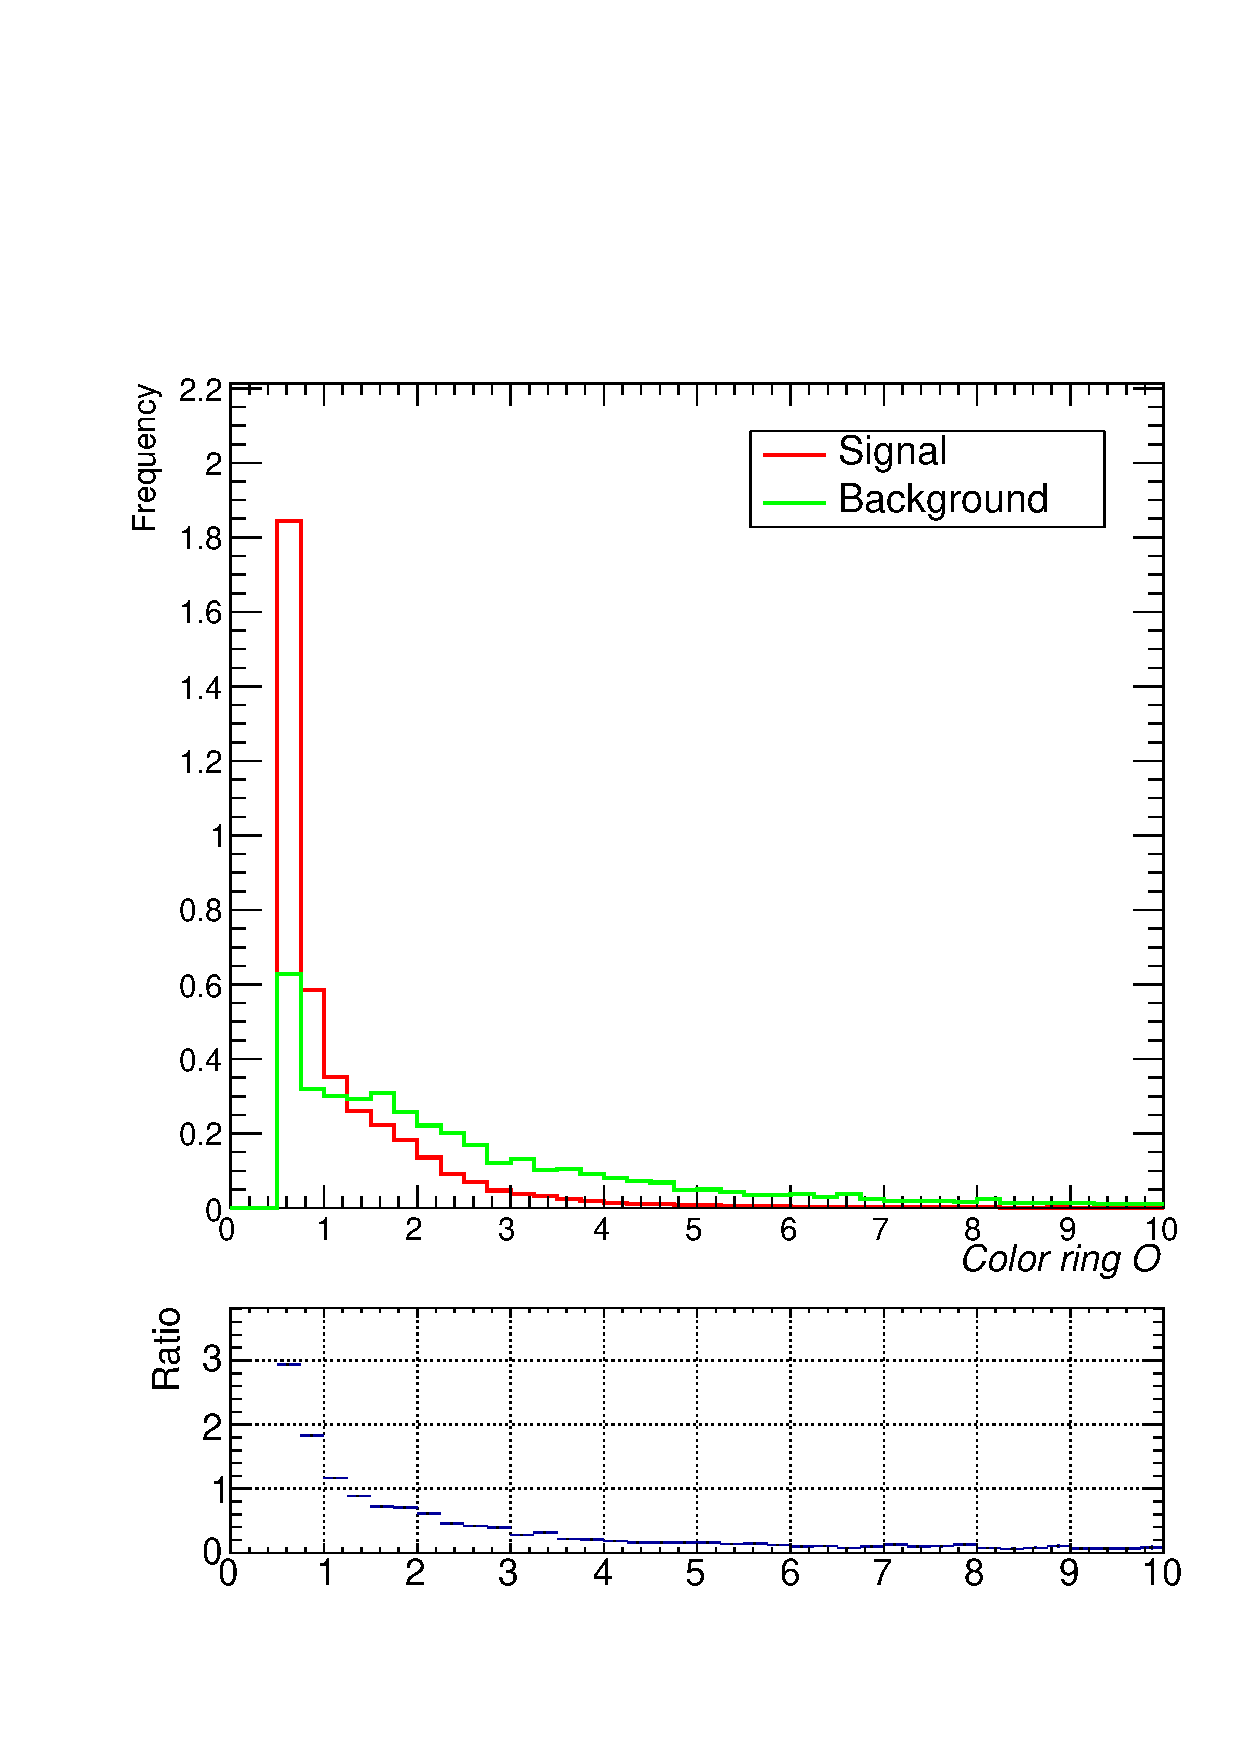
\includegraphics[scale=0.25]{truth/cr}
\caption{$\mathcal{O}$}
\end{subfigure}
\caption{The distributions of the 8 variables after all selection cuts in the truth case together with the ratio between signal and background events.}
\label{sgn/bkg true}
\end{figure}


\begin{figure}
\captionsetup[subfigure]{labelformat=empty}
\begin{subfigure}{.33\textwidth}
\centering
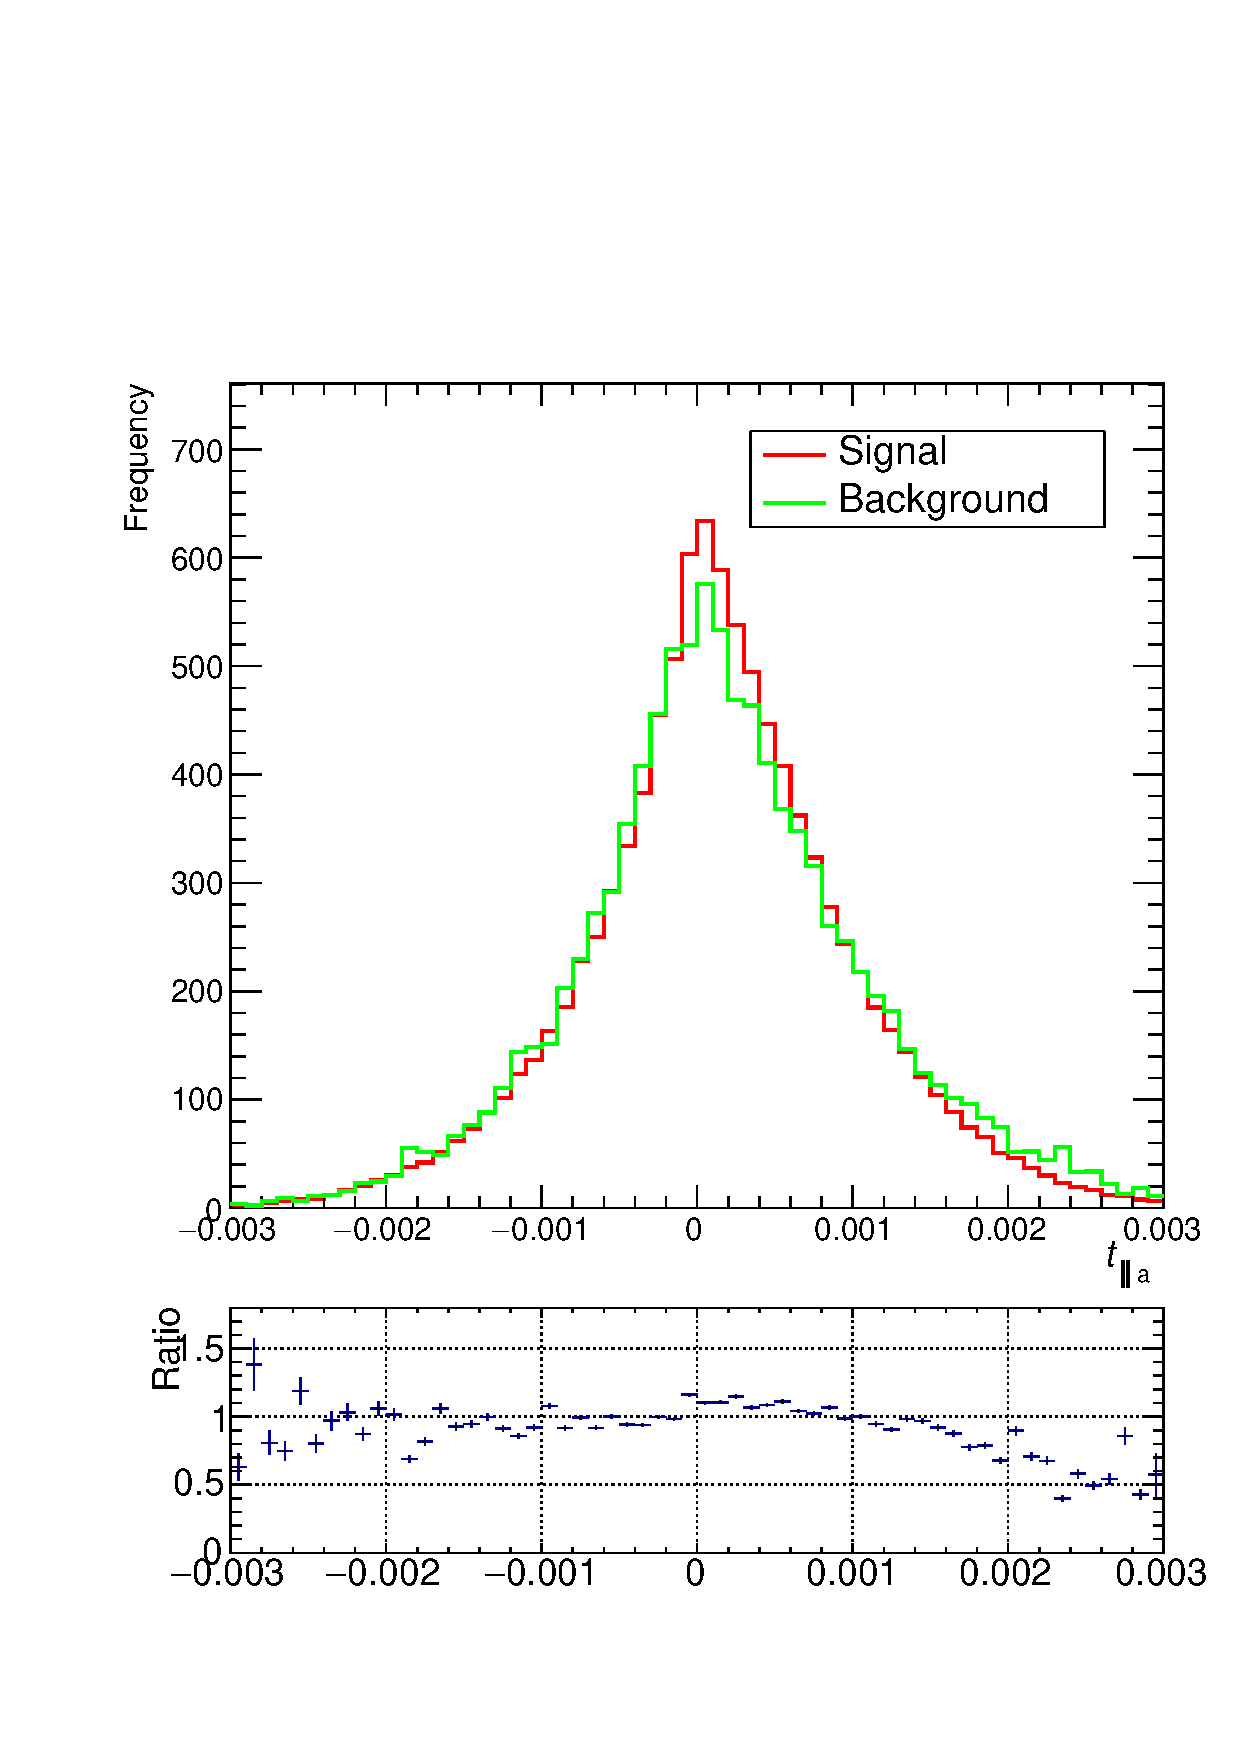
\includegraphics[scale=0.25]{reco/tpar1}
\caption{$t_{\parallel a}$}
\end{subfigure}
\begin{subfigure}{0.33\textwidth}
\centering
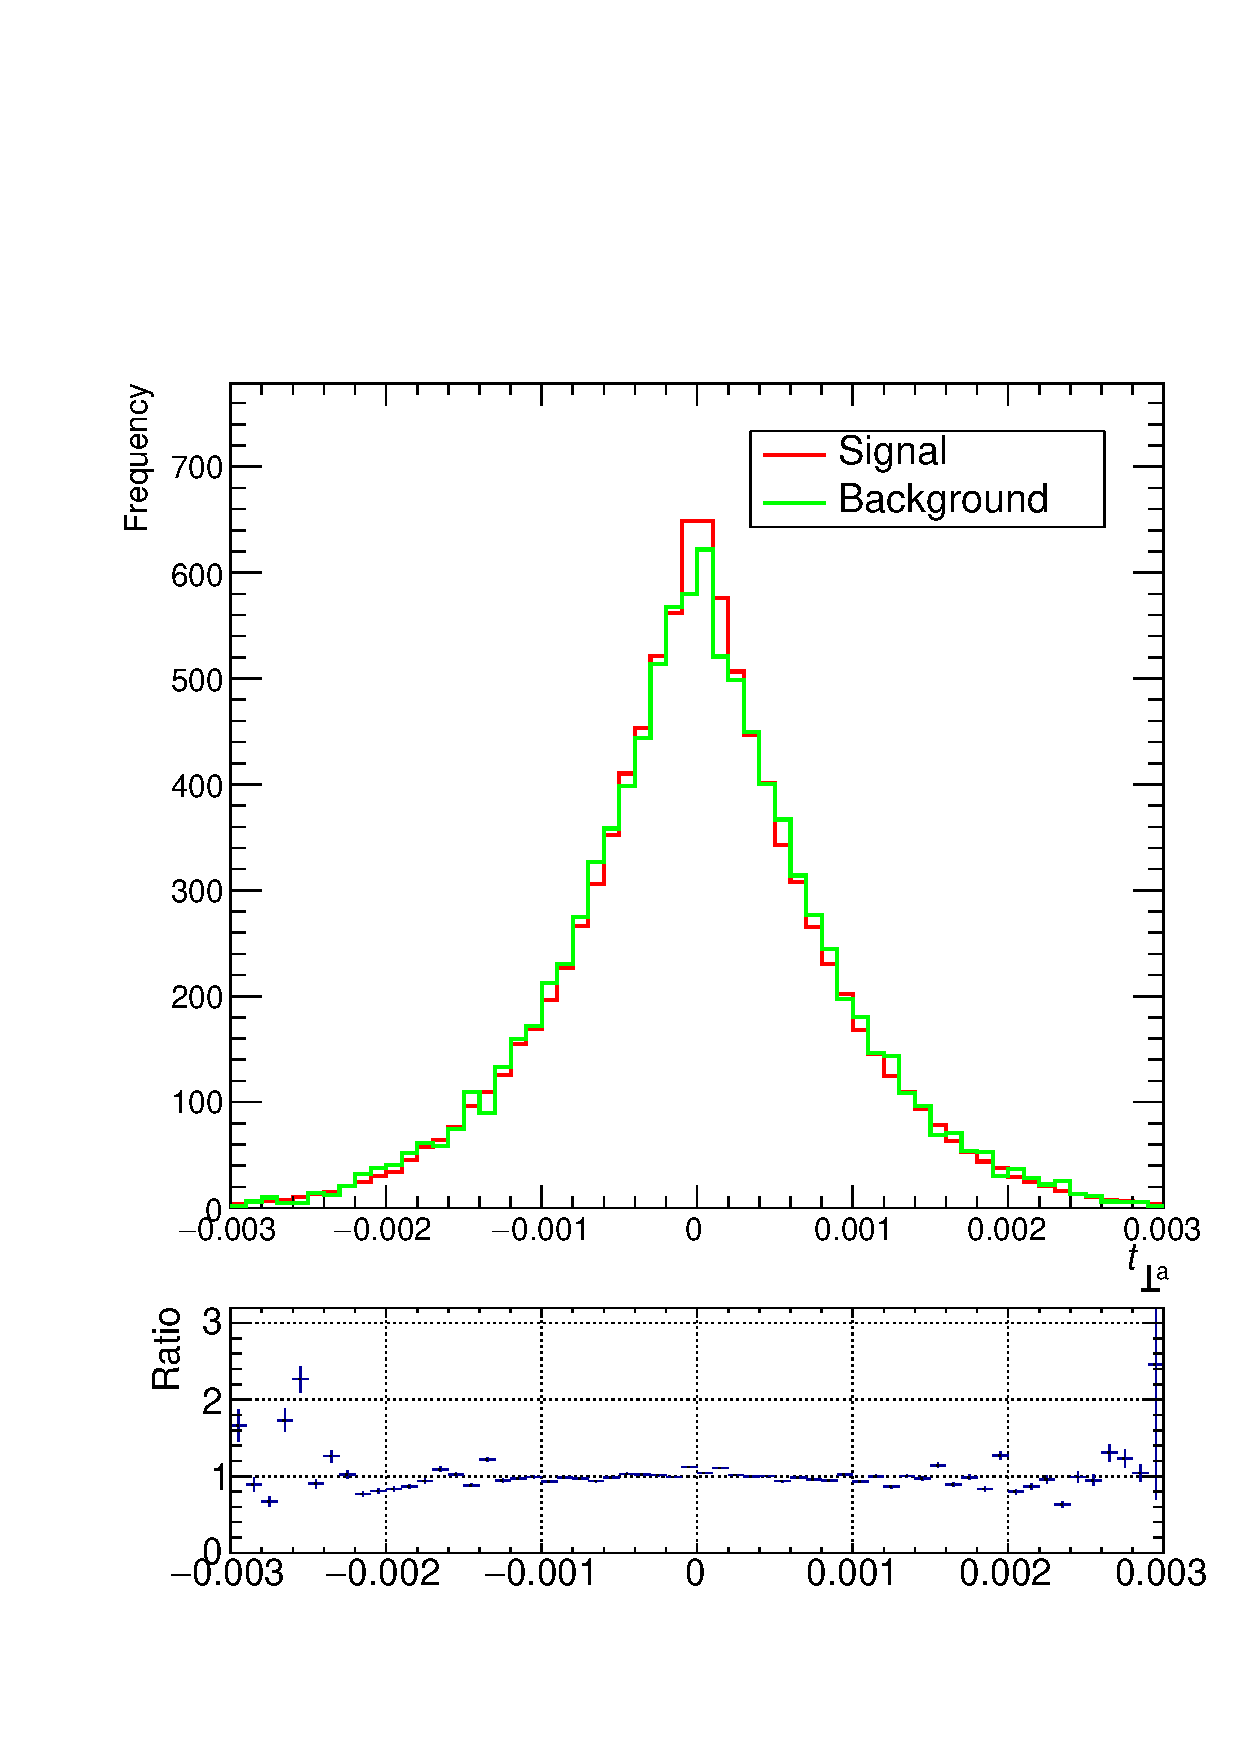
\includegraphics[scale=0.25]{reco/tper1}
\caption{$t_{\perp a}$}
\end{subfigure}
\begin{subfigure}{.33\textwidth}
\centering
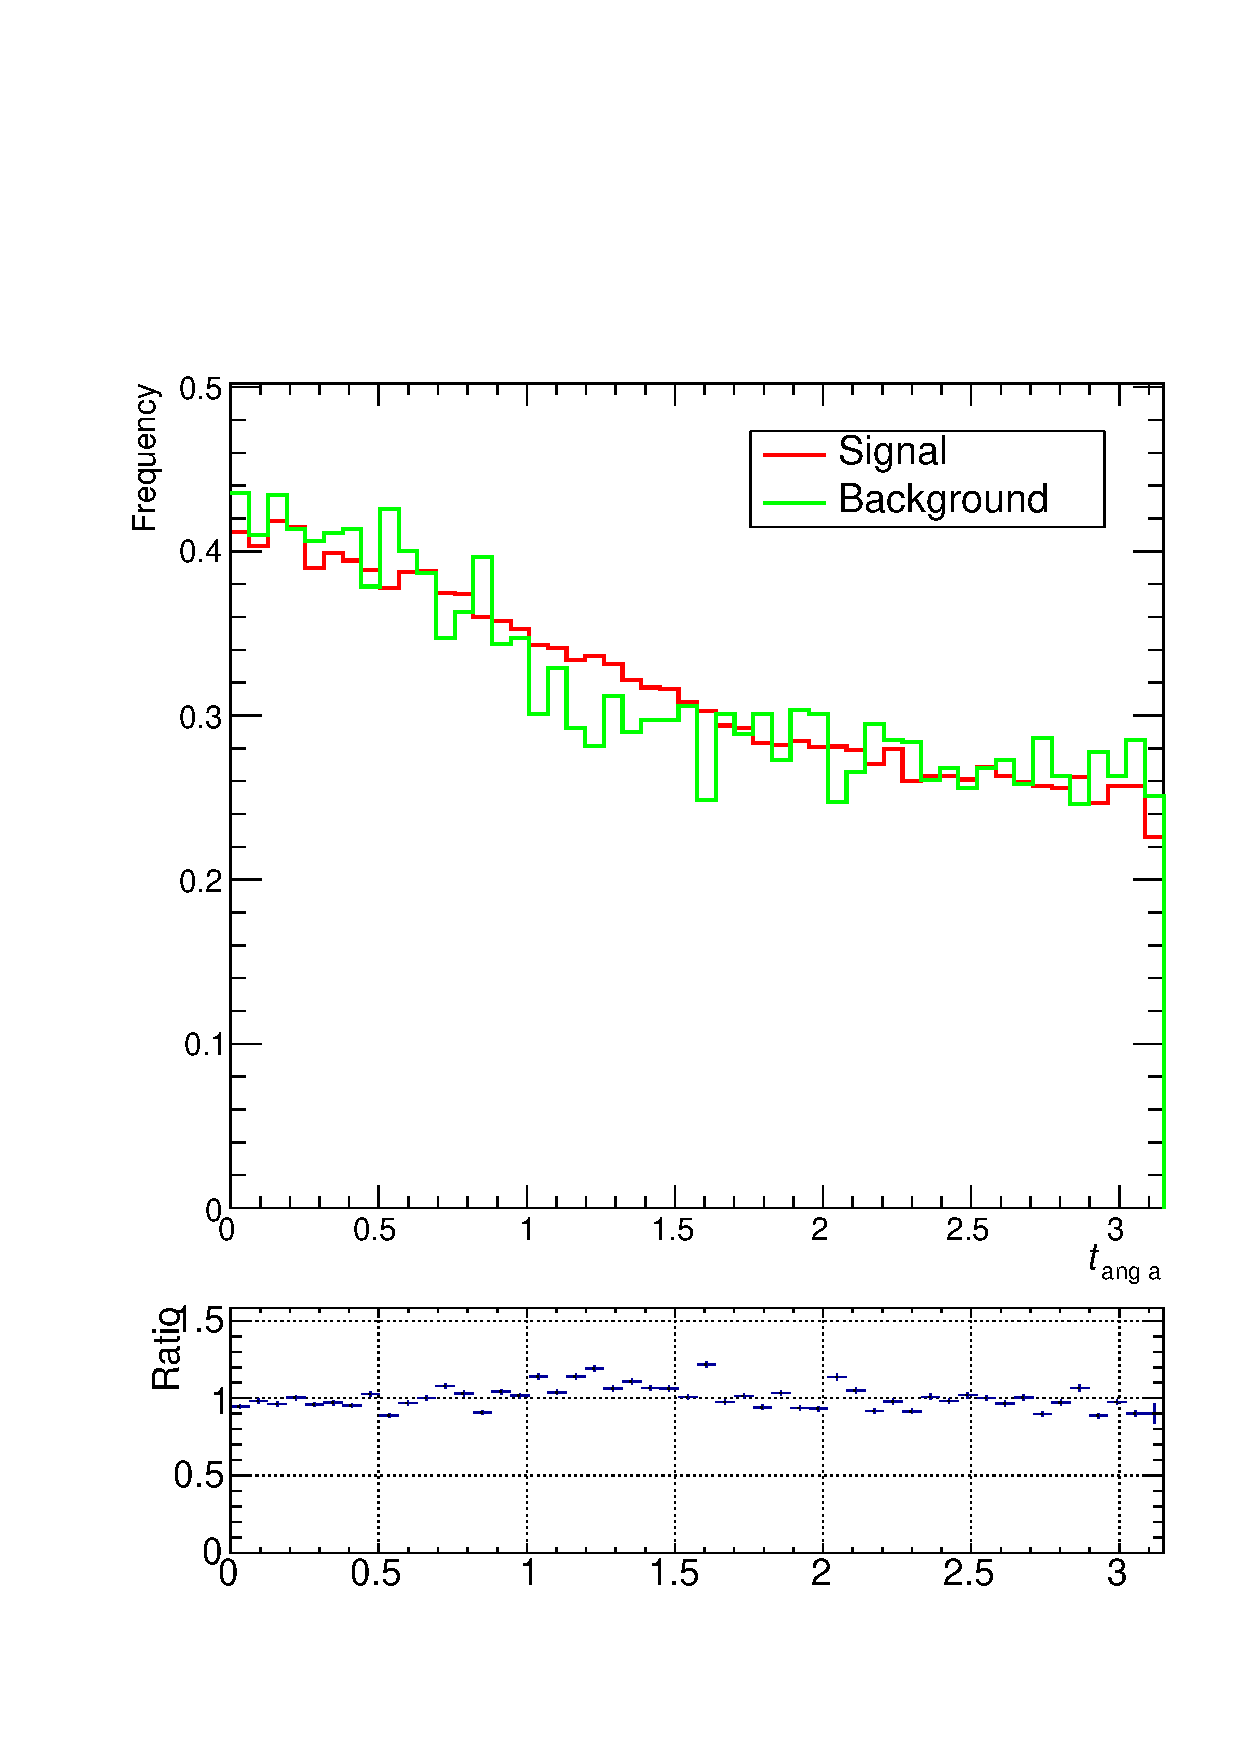
\includegraphics[scale=0.25]{reco/tang1}
\caption{$\theta_{pa}$}
\end{subfigure}
\begin{subfigure}{.33\textwidth}
\centering
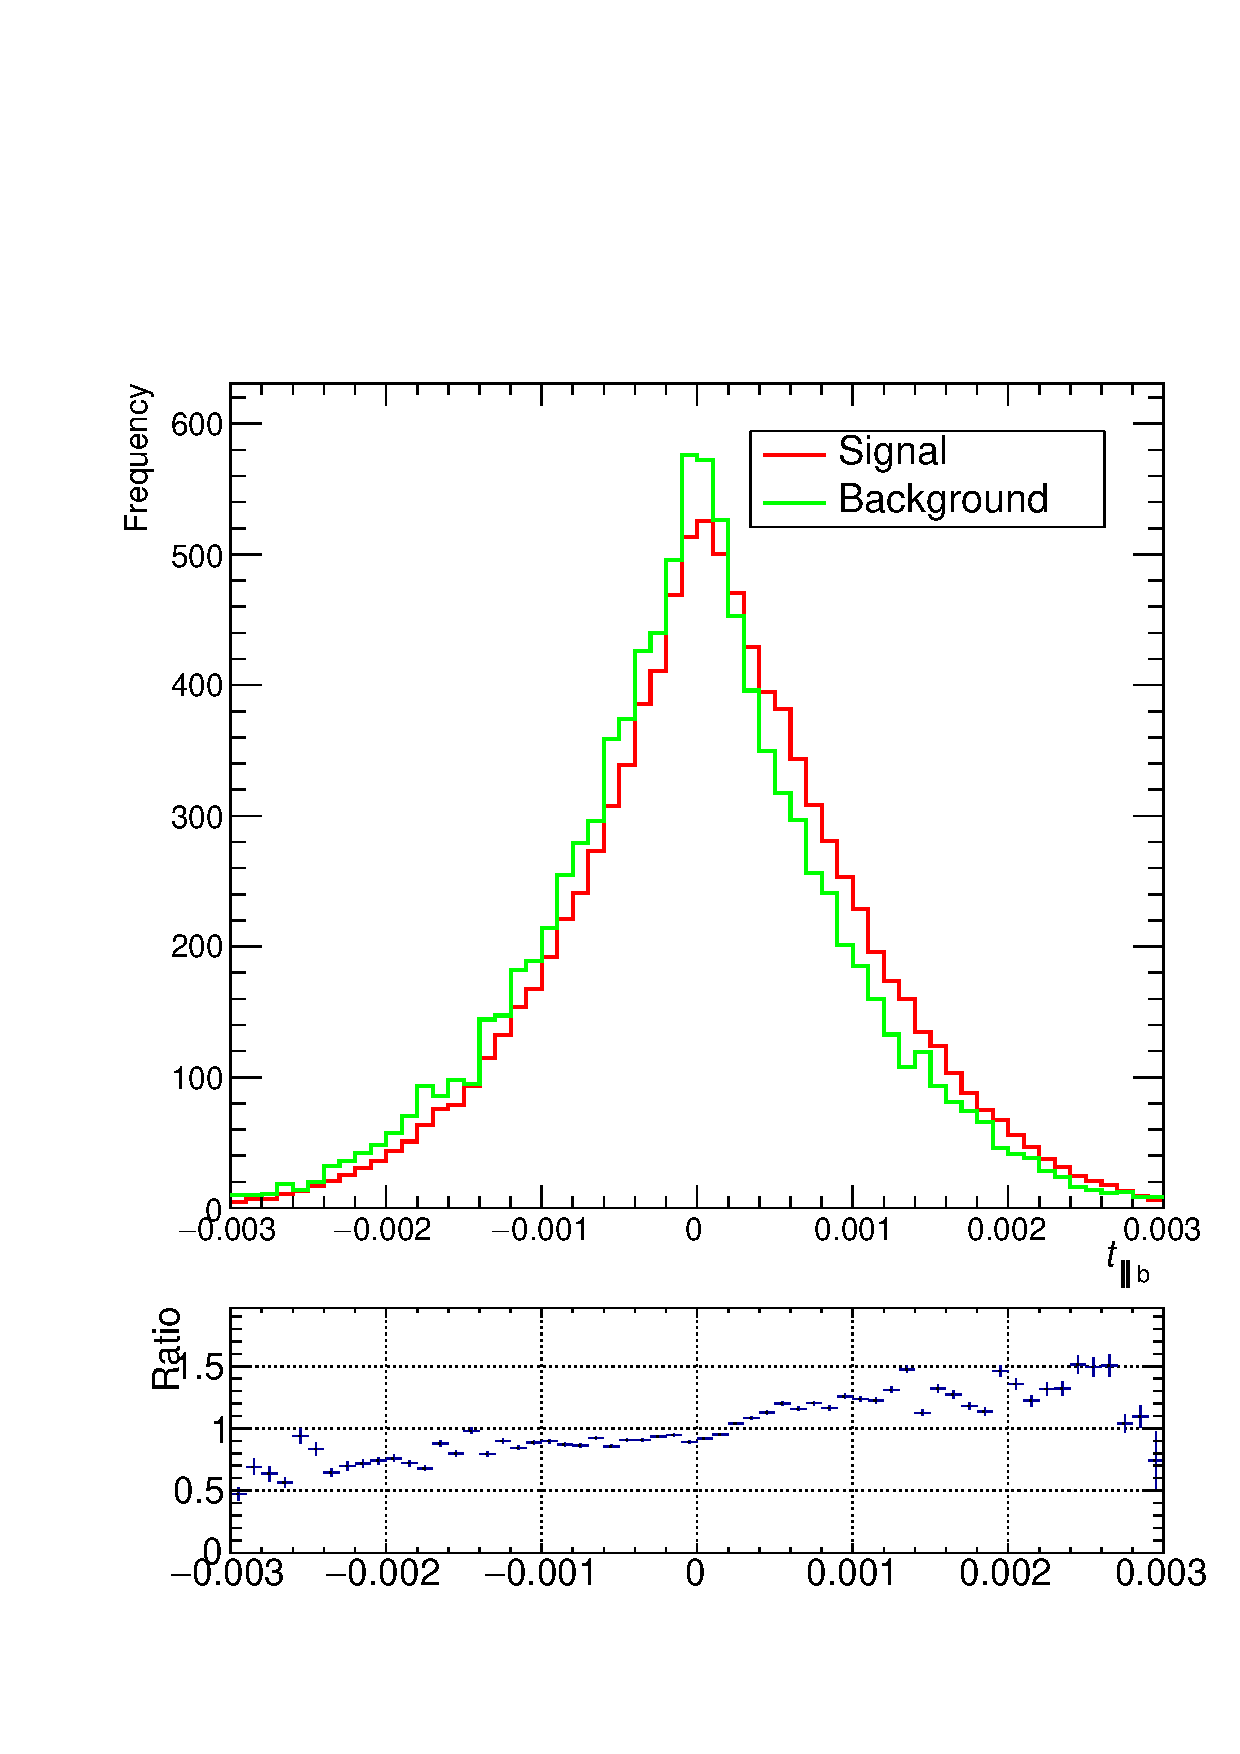
\includegraphics[scale=0.25]{reco/tpar2}
\caption{$t_{\parallel b}$}
\end{subfigure}
\begin{subfigure}{0.33\textwidth}
\centering
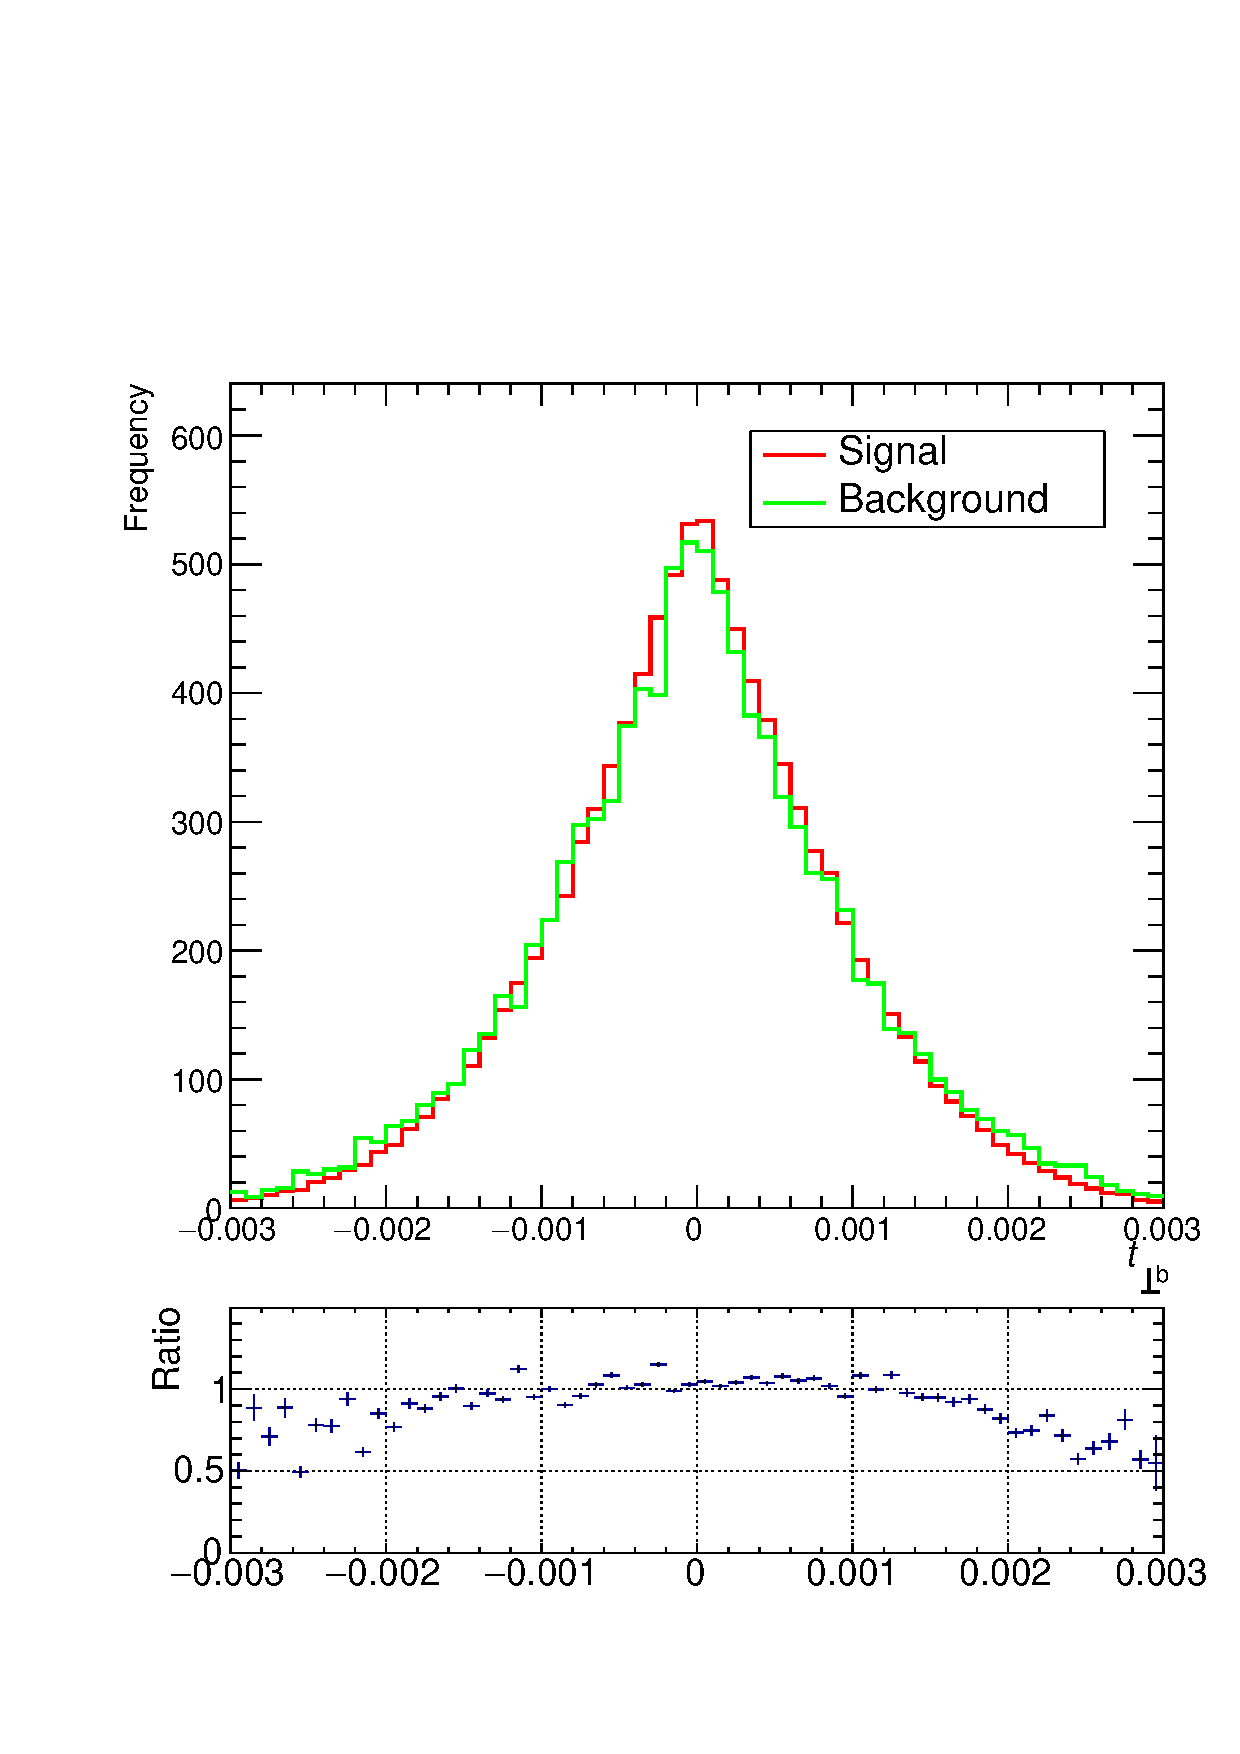
\includegraphics[scale=0.25]{reco/tper2}
\caption{$t_{\perp b}$}
\end{subfigure}
\begin{subfigure}{.33\textwidth}
\centering
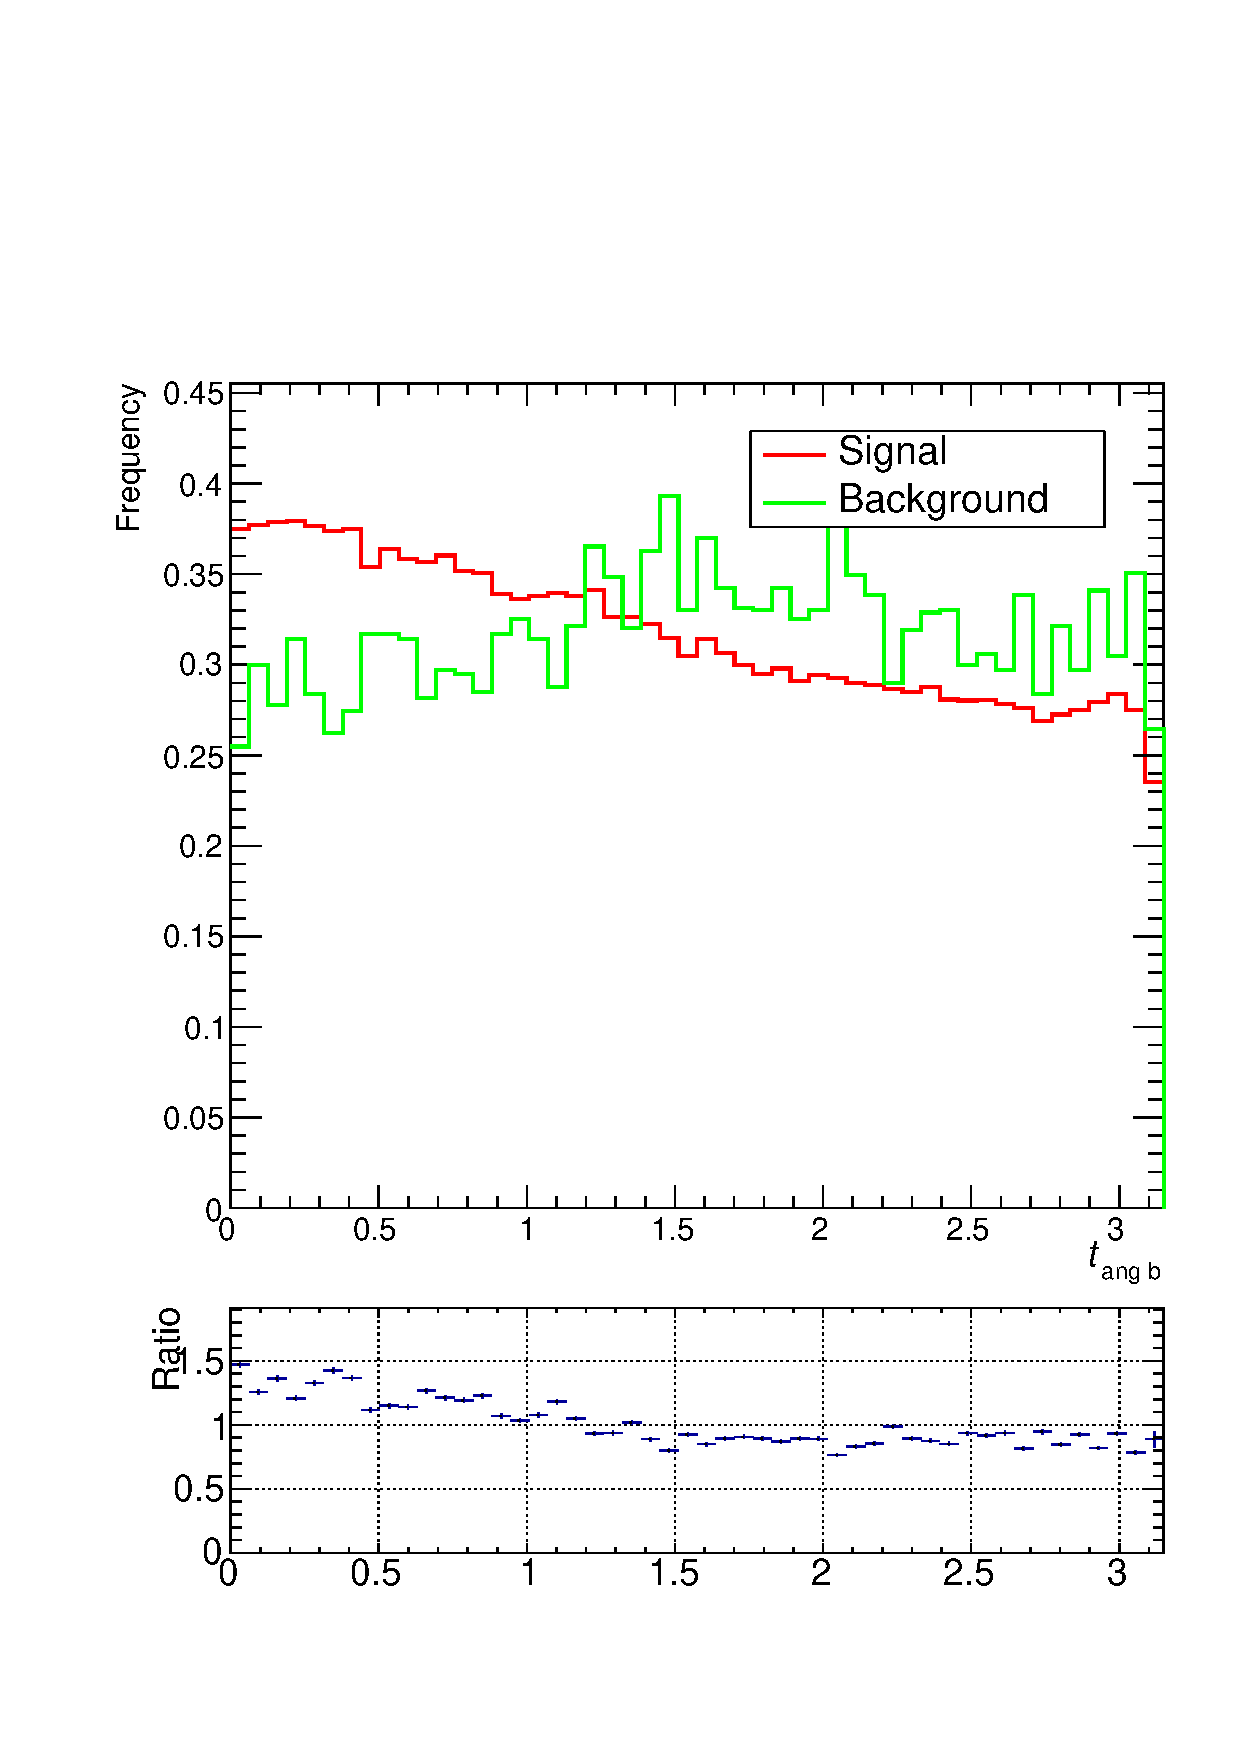
\includegraphics[scale=0.25]{reco/tang2}
\caption{$\theta_{pb}$}
\end{subfigure}
\begin{subfigure}{0.5\textwidth}
\centering
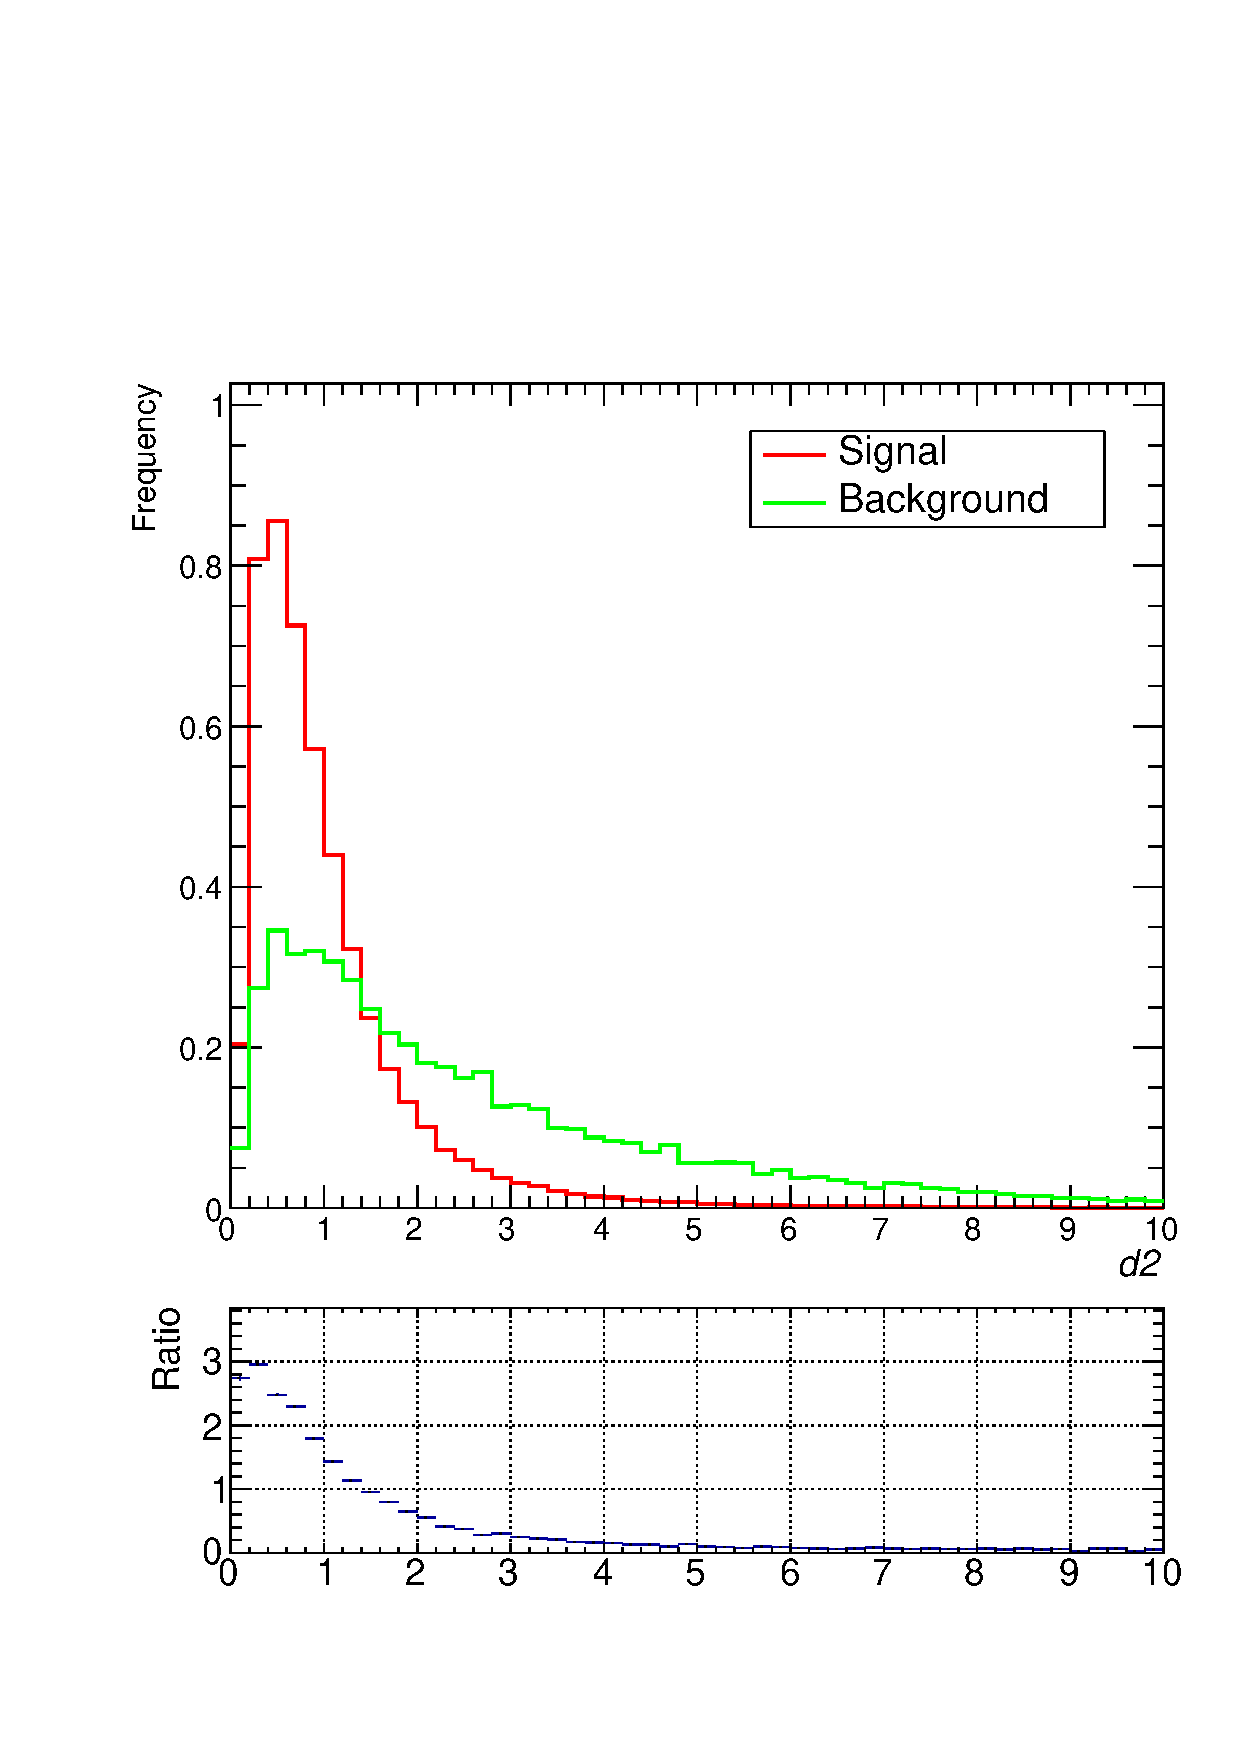
\includegraphics[scale=0.25]{reco/d2}
\caption{$D_2$}
\end{subfigure}
\begin{subfigure}{.5\textwidth}
\centering
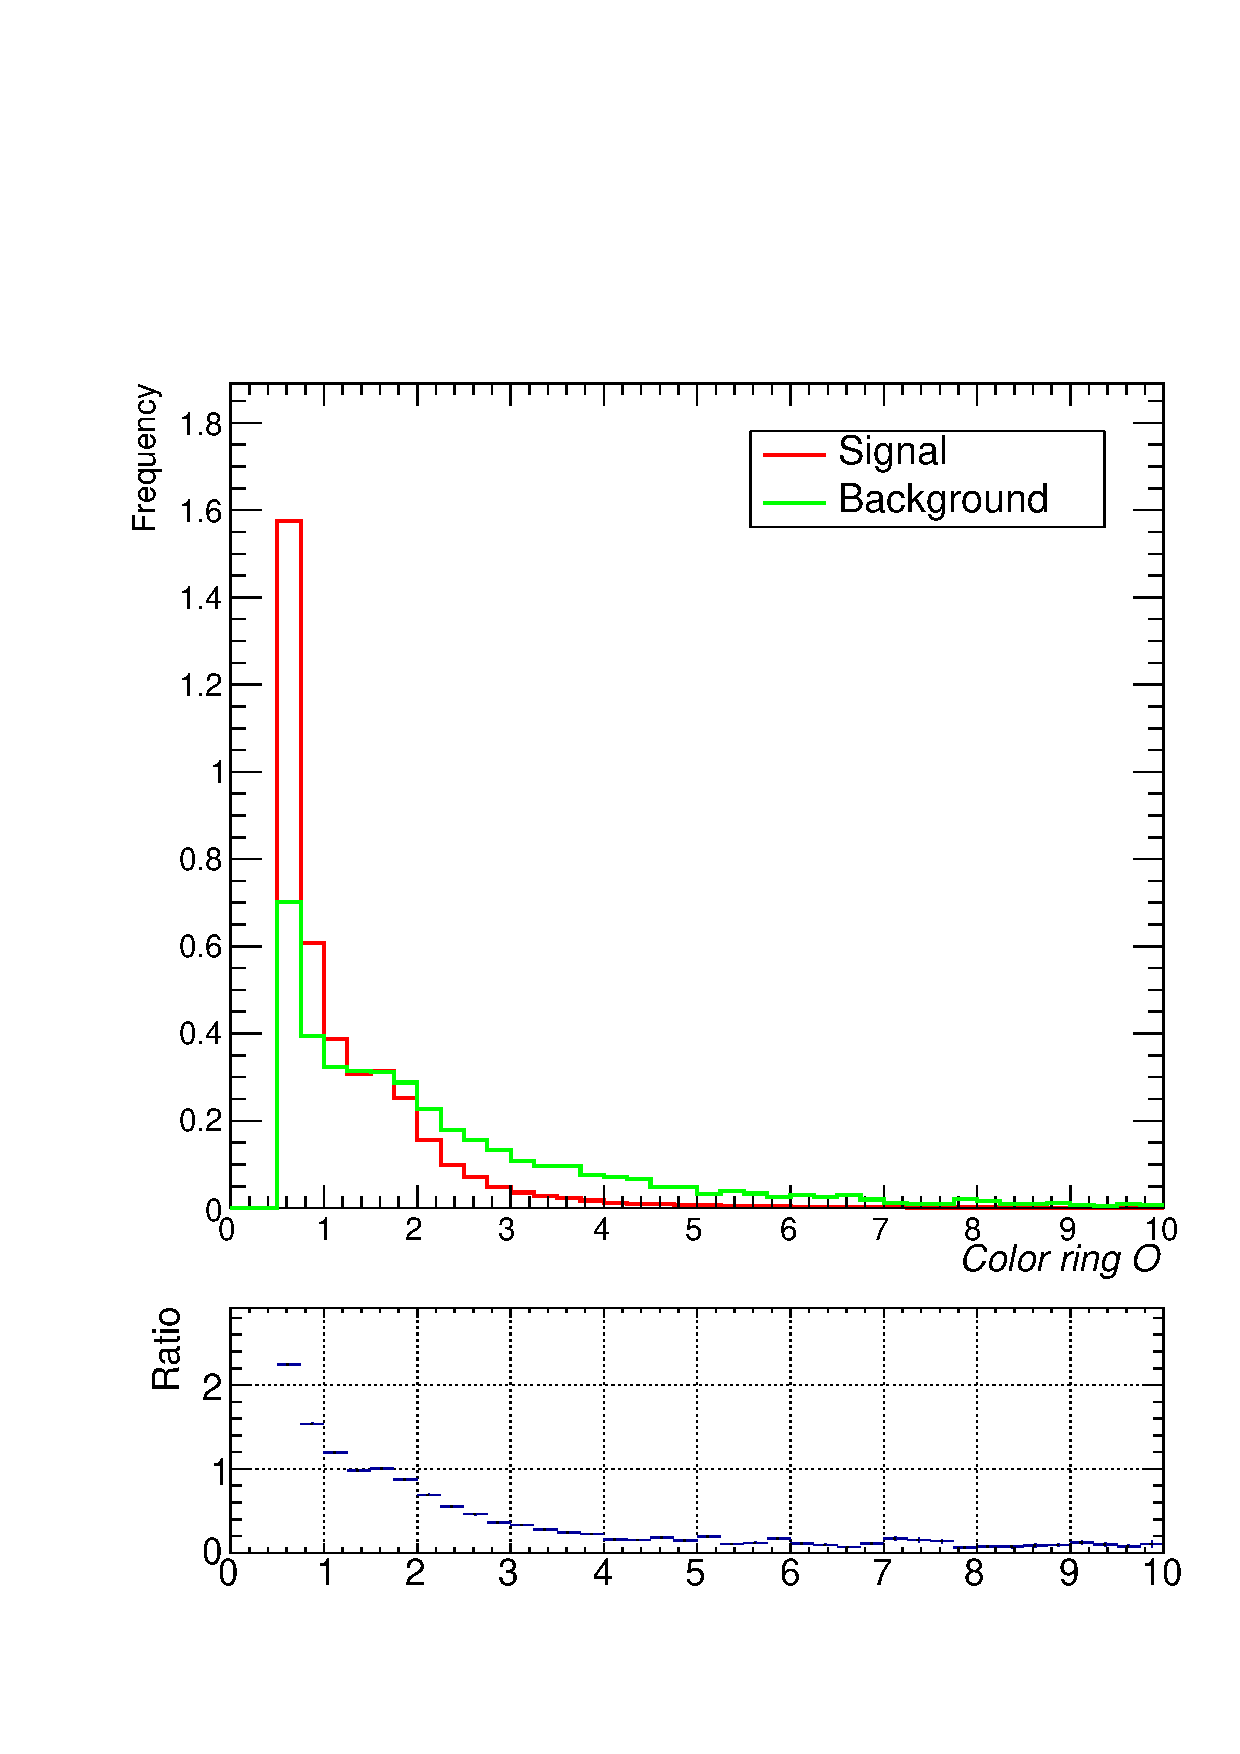
\includegraphics[scale=0.25]{reco/cr}
\caption{$\mathcal{O}$}
\end{subfigure}
\caption{The distributions of the 8 variables after all selection cuts in the reconstructed case together with the ratio between signal and background events.}
\label{sgn/bkg reco}
\end{figure}


\section{Machine Learning Architecture}
The output variables were used to train two different machine learning algorithms: a Multilayer Perceptron (MLP) and Boosted Decision Tree (BDT) from the \code{ROOT} Toolkit for Multivariate Analysis (TMVA) library \cite{TMVA}. In this section, we will limit ourselves to describing the architectures of these algorithms. For a more detailed discussion on how they work, see Appendix \ref{Appendix}.

The MLP is a neural network made of one hidden layer containing nine neurons. All signal and background events are passed to the network in one batch. 50\% of the data is used as a training sample and the other 50\% as a test sample. The number of epochs is set to 600, and a Rectified Linear Unit activation function is used. The learning rate is set to 0.02. 

The BDT is made up of 50 trees, with a maximum depth of 5 and minimum node size set to 2.5\% of the total number of events. The Gini index is used as the optimization criterion. AdaBoost has been chosen as the boosting model and the number of cuts is set to 80. Also in this case, we use a 50/50 train/test sample, and there is no downsampling.


\section{Results}

We are now ready to present our findings. In Figure \ref{ROC curves}, the ROC curves from both the MLP and BDT are shown for the truth and reconstructed cases. The areas under the ROC curves (AUCs) are reported in Table \ref{AUC table}.

\begin{table}[h!]
\centering
\begin{tabular}{|c|c|c|}
\hline 
\* & \multicolumn{2}{c|}{AUC - Test Sample} \\ 
\hline 
\* & Truth & Reco \\ 
\hline 
BDT & 0.818 & 0.777 \\ 
\hline 
MLP & 0.817 & 0.773 \\  
\hline 
\end{tabular} 
\caption{The areas under the ROC curves found.}
\label{AUC table}
\end{table} 

The AUCs show that in the truth case there both machine learning algorithms exhibit good signal/background discrimination. The results are unsurprisingly slightly worse for the reconstructed case due to the introduction of detector effects, but still quite good. This method is thus promising for application to real data.

\begin{figure}[h]
\begin{subfigure}{1.0\textwidth}
\centering
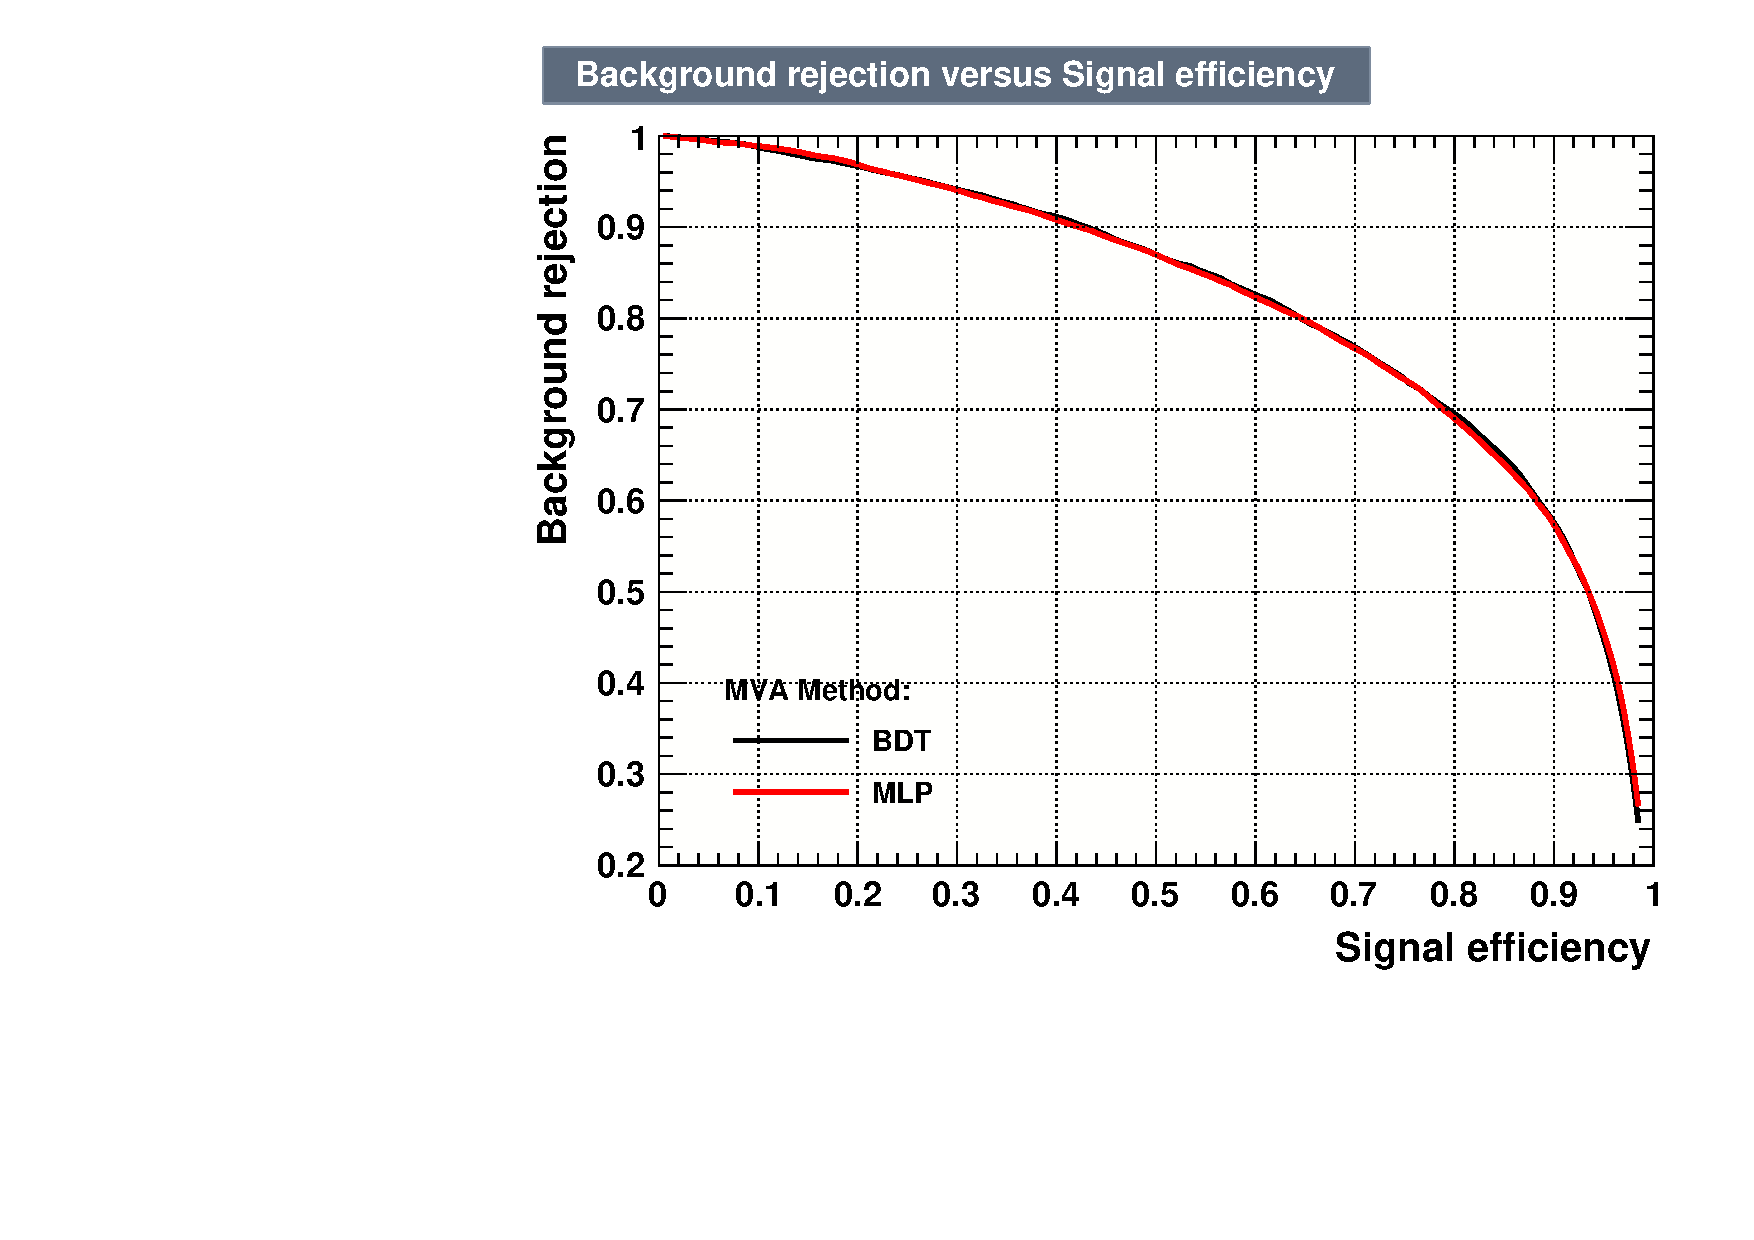
\includegraphics[scale=0.65]{ch4_images/roc_truth}
\caption{}
\end{subfigure}
\begin{subfigure}{1.0\textwidth}
\centering
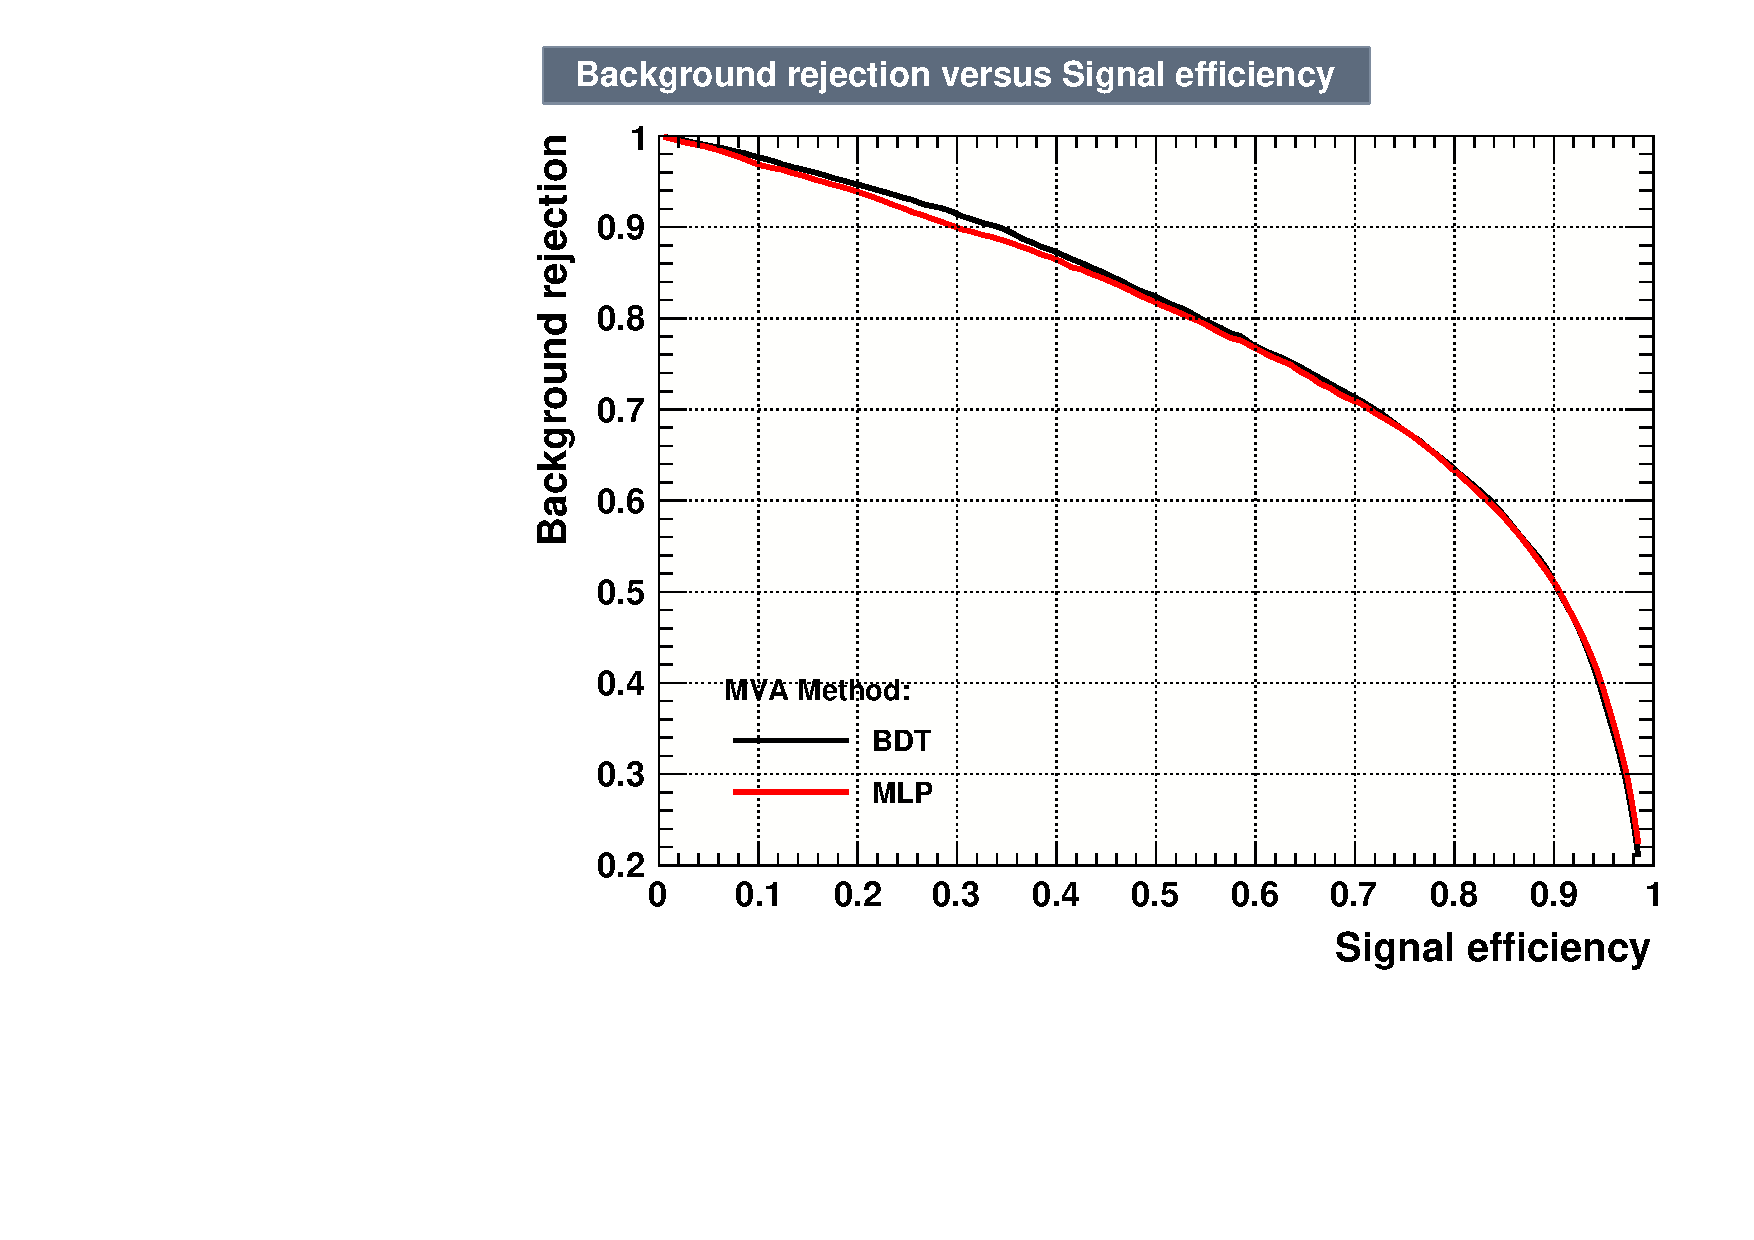
\includegraphics[scale=0.65]{ch4_images/roc_reco.pdf}
\caption{}
\end{subfigure}
\caption{The ROC curves showing background rejection as a function of signal efficiency for the truth case (a) and for the reconstructed case (b) for both the BDT and the MLP.}
\label{ROC curves}
\end{figure} 

We can also rank the variables based on their importance. The ranking for the BDT is reported in Table \ref{variable ranking}. $D_2$ is the most discriminant variable, and the others are all of similar importance. For the reconstructed case, $\mathcal{O}$ gains additional importance with respect to the pull variables.

\begin{table}
    \begin{minipage}{.5\linewidth}
      %\caption{}
      \centering
        \begin{tabular}{|c|c|c|}
	\hline 
	\multicolumn{3}{|c|}{Variable Ranking - Truth} \\ 
	\hline 
	Rank & Var. & Importance \\ 
	\hline 
	1 & $D_2$ & 3.743$\times 10^{-1}$ \\ 
	\hline 
	2 & $\theta_{pb}$ & 1.083$\times 10^{-1}$ \\ 
	\hline 
	3 & $t_{\parallel a}$ & 9.508$\times 10^{-2}$ \\ 
	\hline 
	4 & $\theta_{pa}$ & 9.506$\times 10^{-2}$ \\ 
	\hline 
	5 & $t_{\parallel b}$ & 9.729$\times 10^{-2}$ \\ 
	\hline 
	6 & $\mathcal{O}$  & 8.637$\times 10^{-2}$ \\ 
	\hline 
	7 & $t_{\perp b}$ & 8.151$\times 10^{-2}$ \\ 
	\hline 
	8 & $t_{\perp a}$& 7.206$\times 10^{-2}$ \\ 
	\hline 
	\end{tabular} 
    \end{minipage}%
    \begin{minipage}{.5\linewidth}
      \centering
        %\caption{}
        \begin{tabular}{|c|c|c|}
	\hline 
	\multicolumn{3}{|c|}{Variable Ranking - Reco} \\ 
	\hline 
	Rank & Var. & Importance \\ 
	\hline 
	1 & $D_2$ & 3.536$\times 10^{-1}$ \\ 
	\hline 
	2 & $\mathcal{O}$ & 1.116$\times 10^{-1}$ \\ 
	\hline 
	3 & $\theta_{pa}$ & 1.020$\times 10^{-1}$ \\ 
	\hline 
	4 & $t_{\perp b}$ & 9.347$\times 10^{-2}$ \\ 
	\hline 
	5 & $t_{\perp a}$ & 9.137$\times 10^{-2}$ \\ 
	\hline 
	6 & $t_{\parallel a}$  & 8.795$\times 10^{-2}$ \\ 
	\hline 
	7 & $\theta_{pb}$ & 8.136$\times 10^{-2}$ \\ 
	\hline 
	8 & $t_{\parallel b}$ & 7.862$\times 10^{-2}$ \\ 
	\hline 
	\end{tabular}  
    \end{minipage} 
    \caption{The importance of the variables found by the BDT using the data from the truth case and the reconstructed case.}
    \label{variable ranking}
\end{table}


Figure \ref{correlation reco} shows the correlation between the variables for the signal and for the background in the reconstructed case. Unsurprisingly, $t_{\parallel a}$ is correlated with $\theta_{pa}$ and $t_{\parallel b}$ is correlated with $\theta_{pb}$, as they are related to each other by definition. There is also some correlation present between $D_2$ and $\mathcal{O}$ in the background. 

\begin{figure}[h]
\begin{subfigure}{1.0\textwidth}
\centering
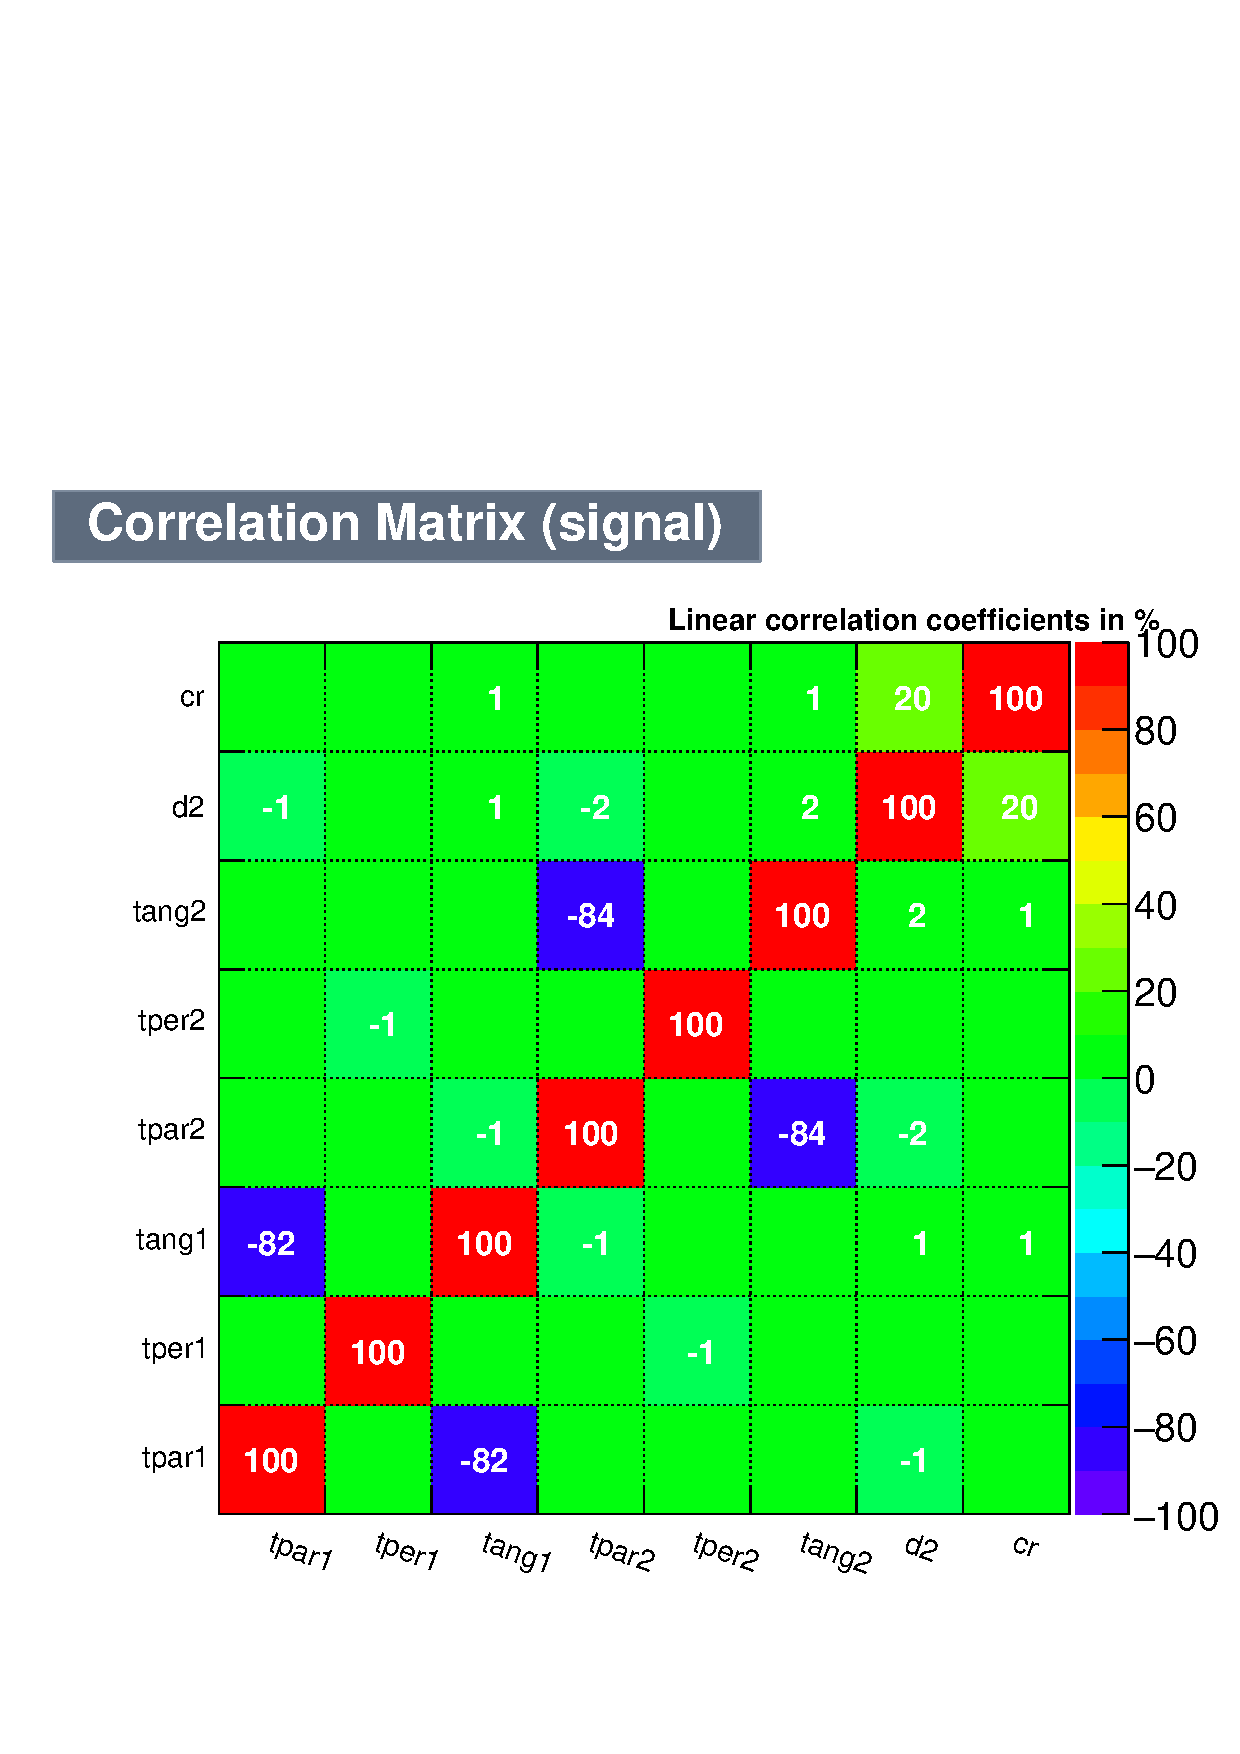
\includegraphics[width=0.7\textwidth]{ch4_images/CorrelationMatrixS_reco.pdf}
\caption{}
\end{subfigure}
\begin{subfigure}{1.0\textwidth}
\centering
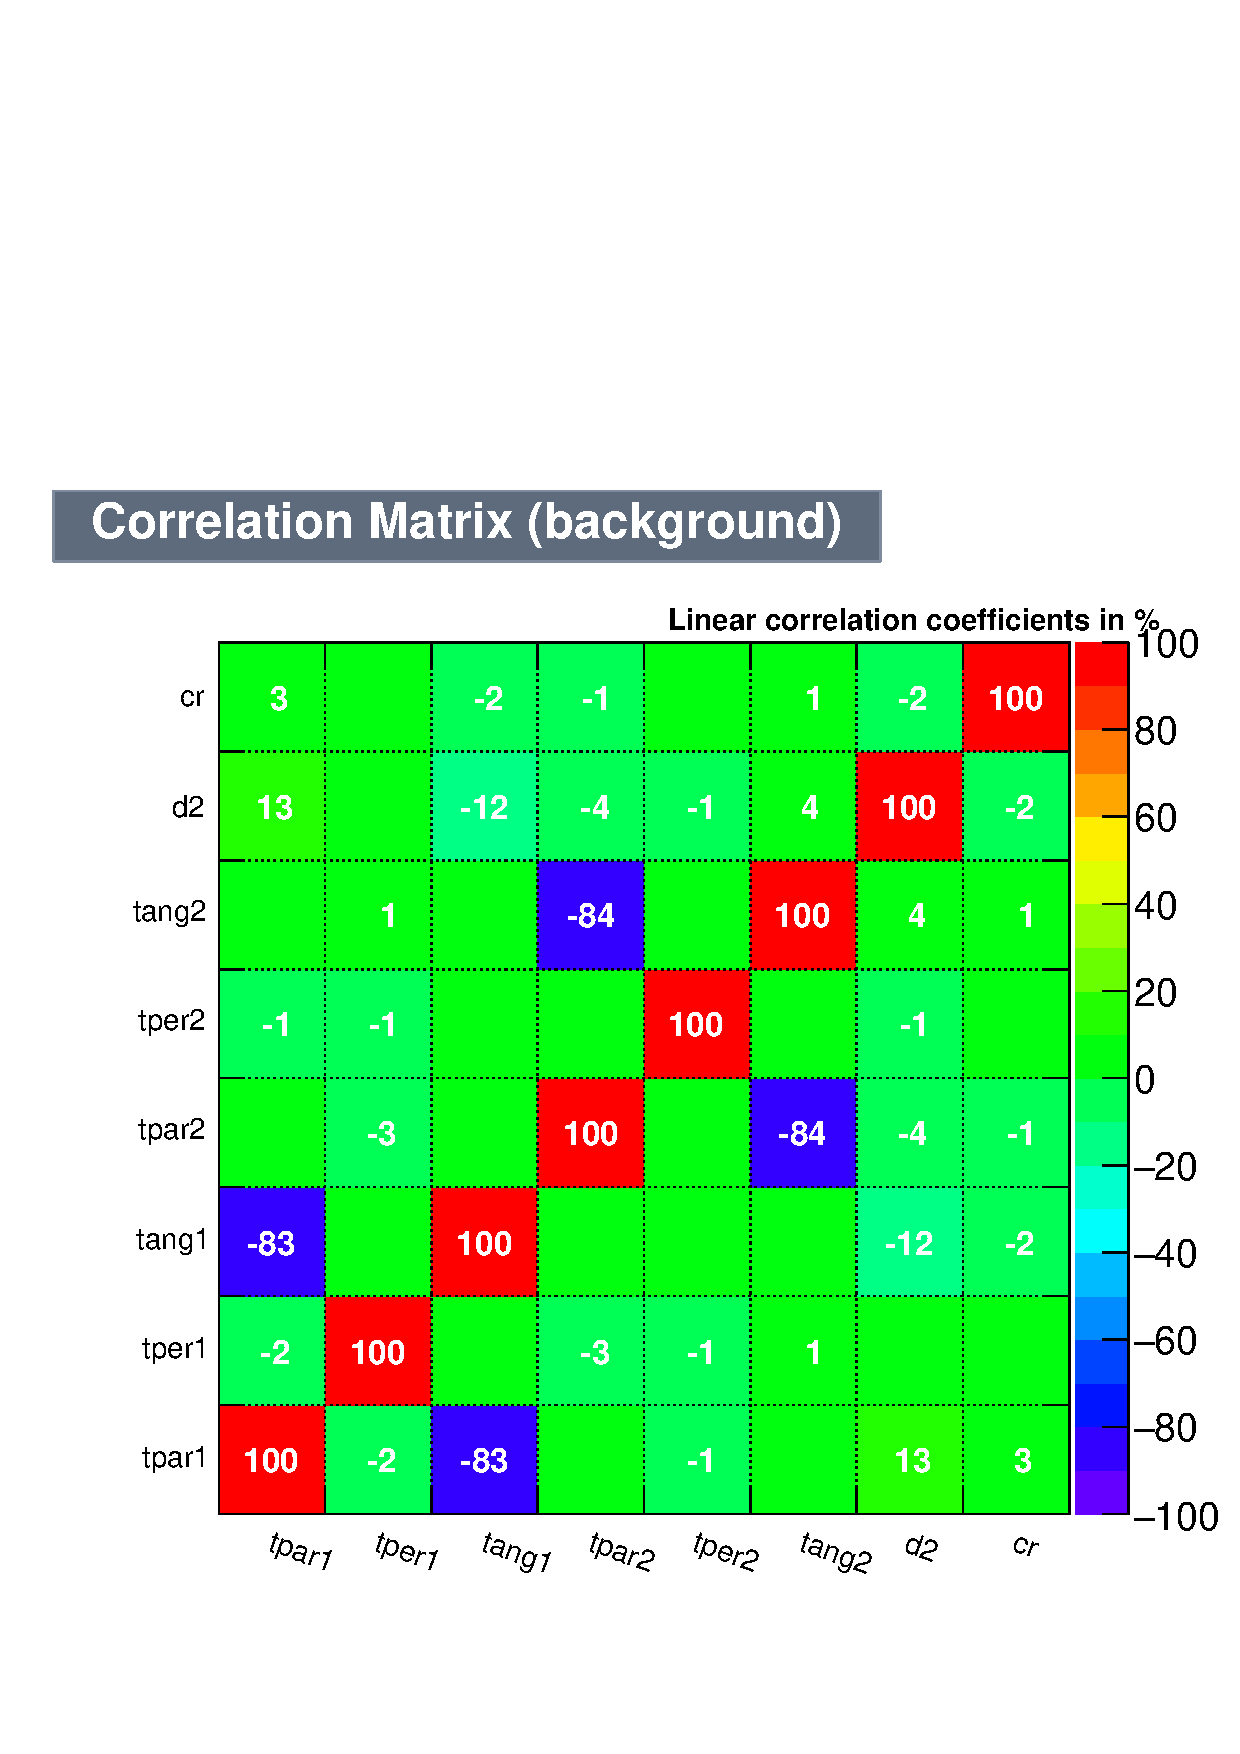
\includegraphics[width=0.7\textwidth]{ch4_images/CorrelationMatrixB_reco.pdf}
\caption{}
\end{subfigure}
\caption{The correlation matrix found by the MLP in the reconstructed case for the signal (a) and for the background (b).}
\label{correlation reco}
\end{figure} 

Finally, Figures \ref{kolmogorov smirnov mlp} and \ref{kolmogorov smirnov bdt} show the result of a Kolmogorov-Smirnov test \cite{10.2307/2280095} performed on the MLP and the BDT to check for overfitting. Since the test probability $\rho_{KS} > 0.01$ in all cases, no overtraining has occurred.

\begin{figure}[h]
\begin{subfigure}{0.8\textwidth}
\centering
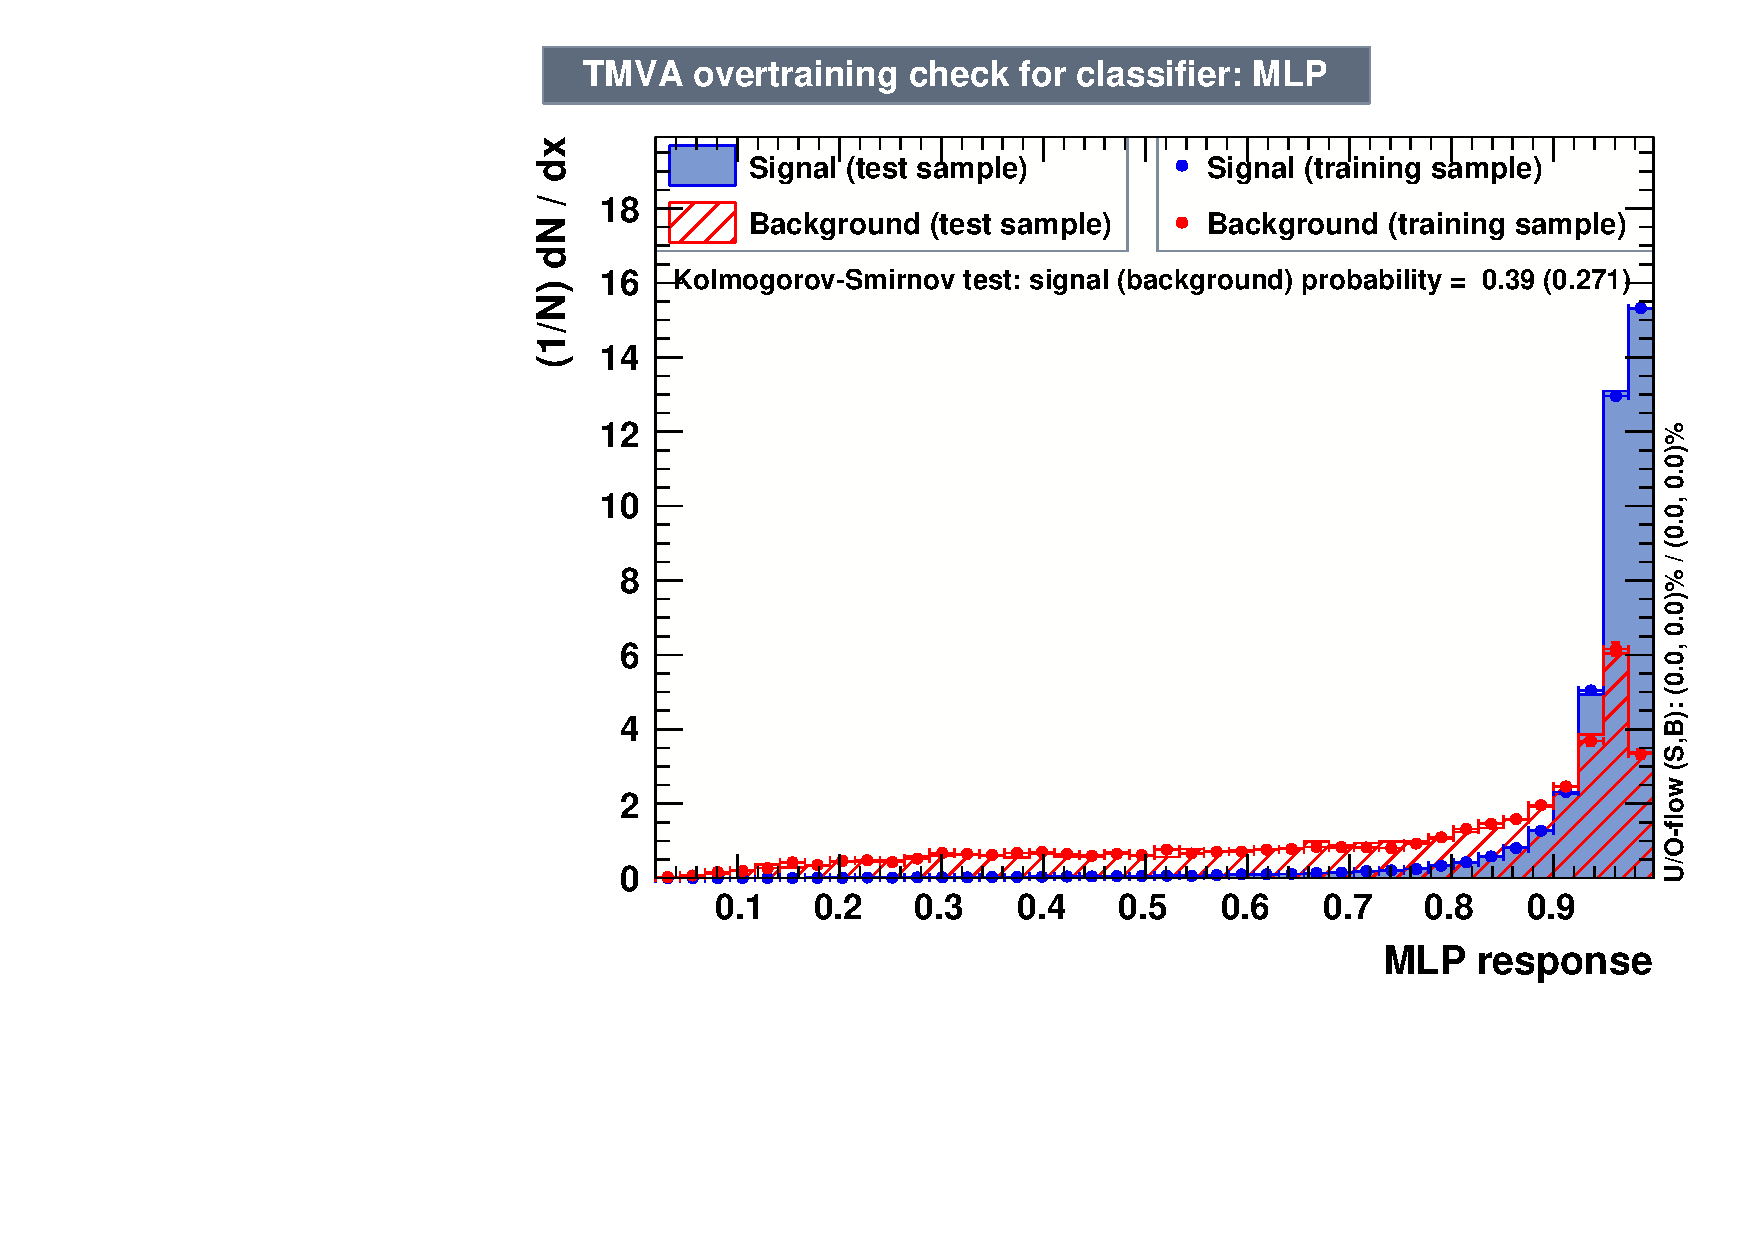
\includegraphics[width=\textwidth]{ch4_images/ks_mlp_truth.pdf}
\caption{}
\end{subfigure}
\begin{subfigure}{0.8\textwidth}
\centering
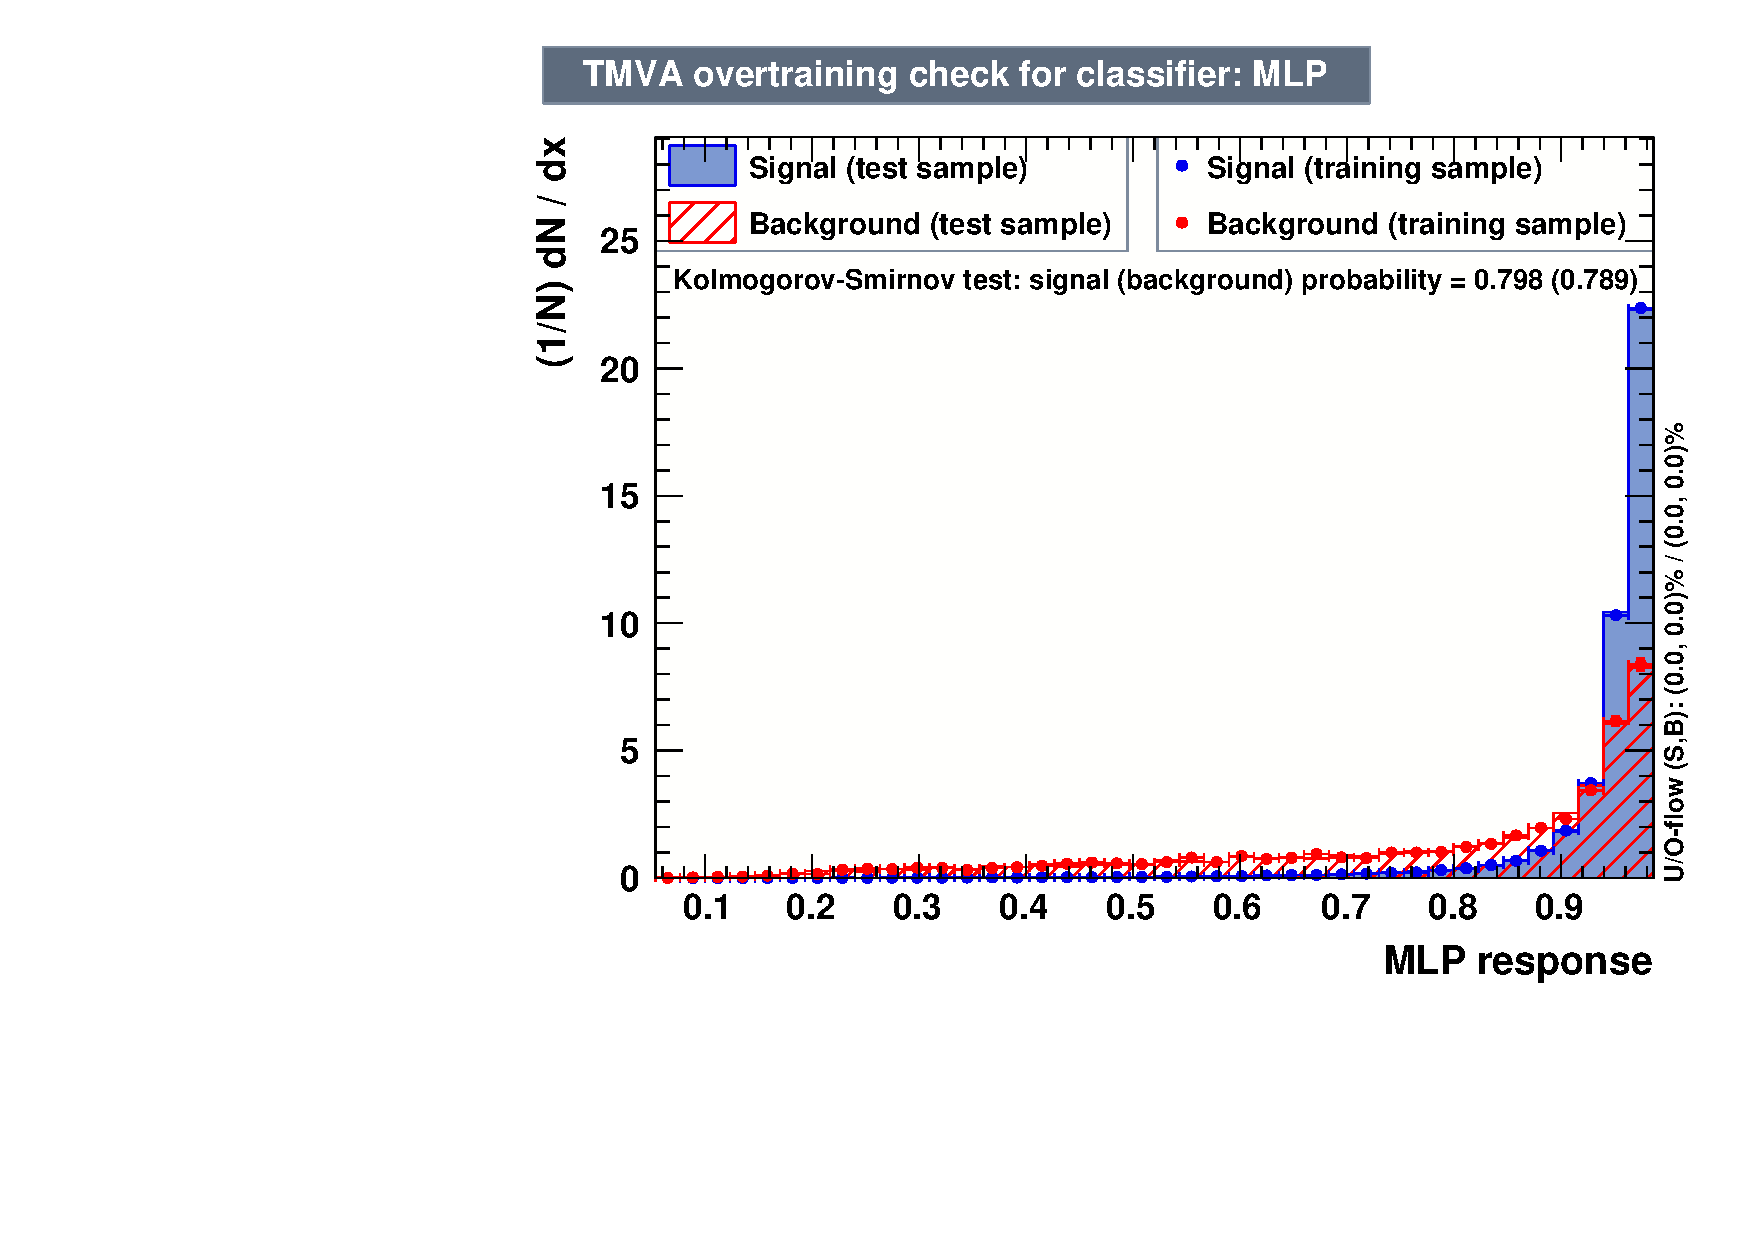
\includegraphics[width=\textwidth]{ch4_images/ks_mlp_reco.pdf}
\caption{}
\end{subfigure}
\caption{The result of a Kolmogorov-Smirnov test performed on the MLP in the truth case (a) and the reconstructed case (b).}
\label{kolmogorov smirnov mlp}
\end{figure} 

\begin{figure}[h]
\begin{subfigure}{0.8\textwidth}
\centering
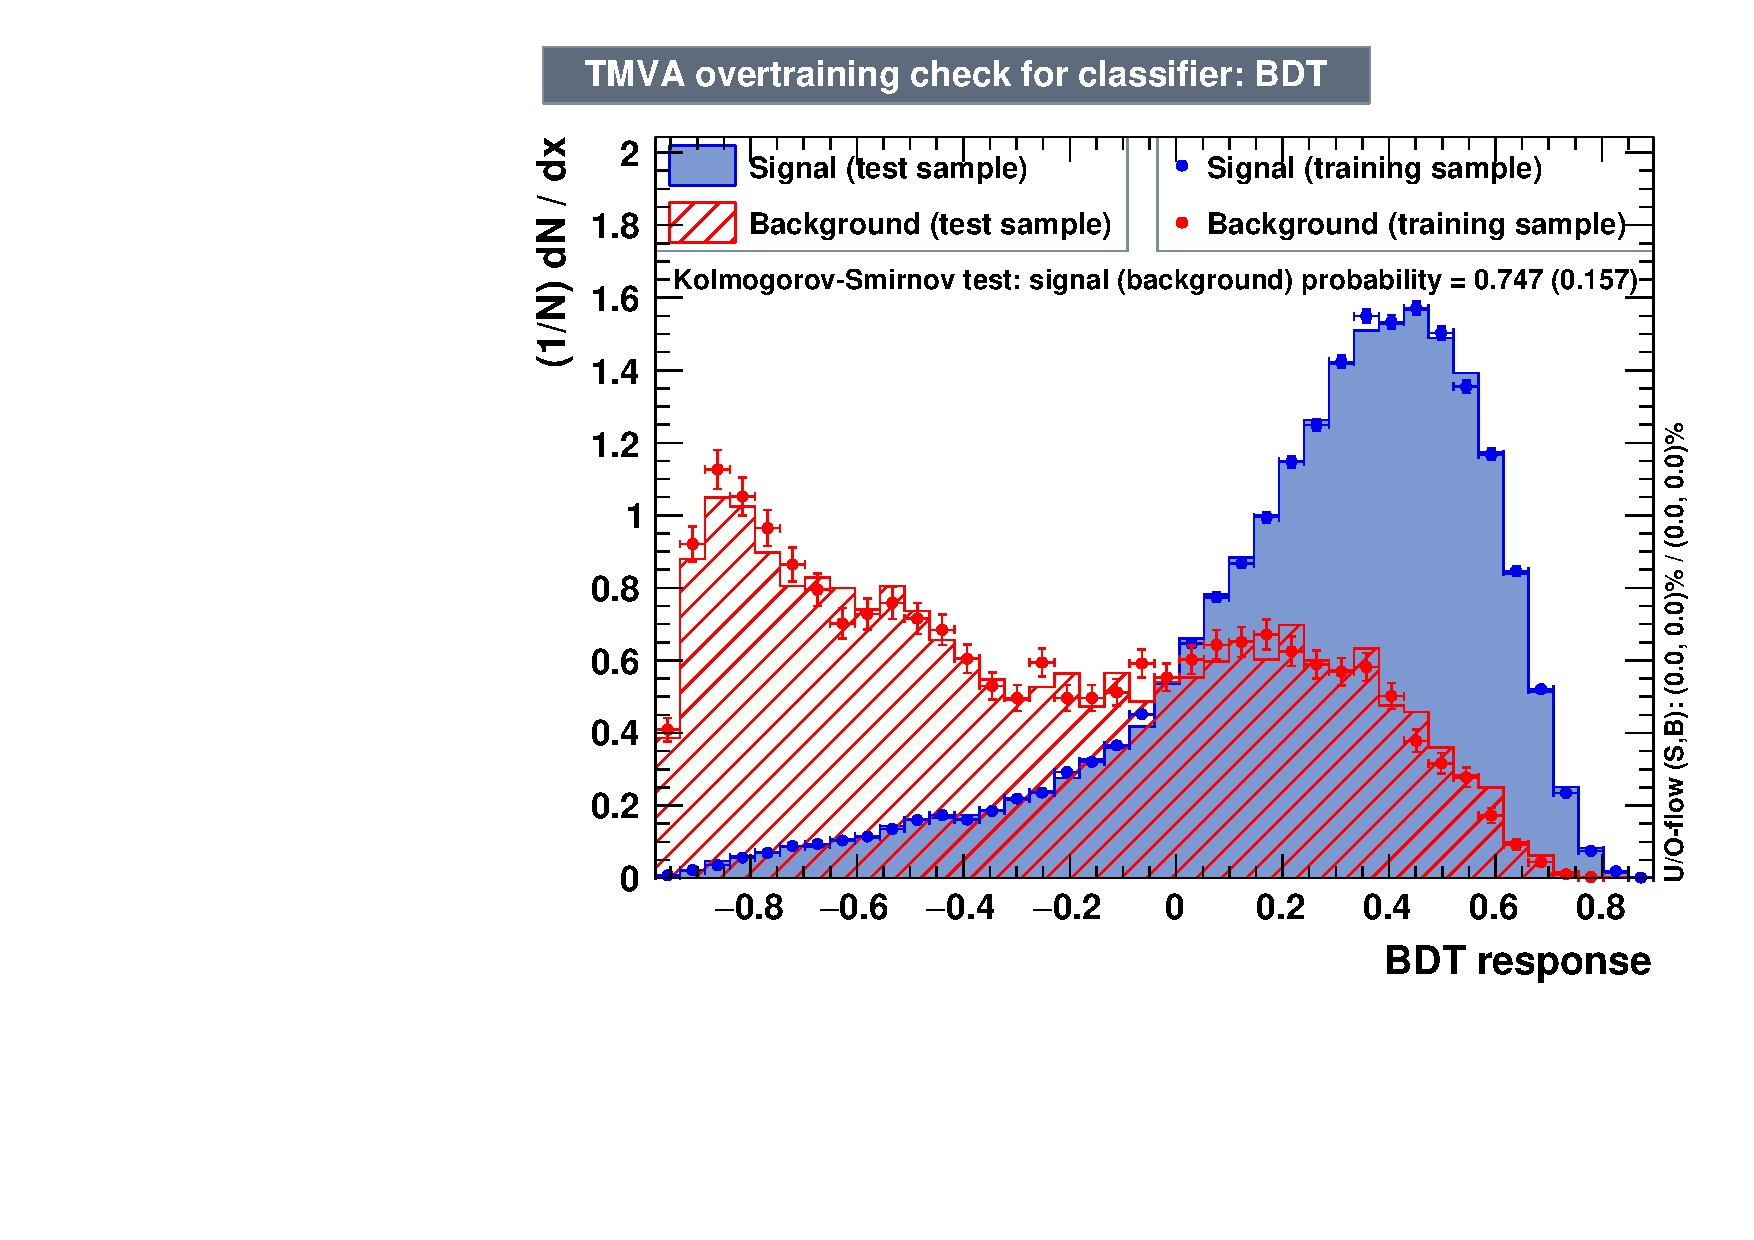
\includegraphics[width=\textwidth]{ch4_images/ks_bdt_truth}
\caption{}
\end{subfigure}
\begin{subfigure}{0.8\textwidth}
\centering
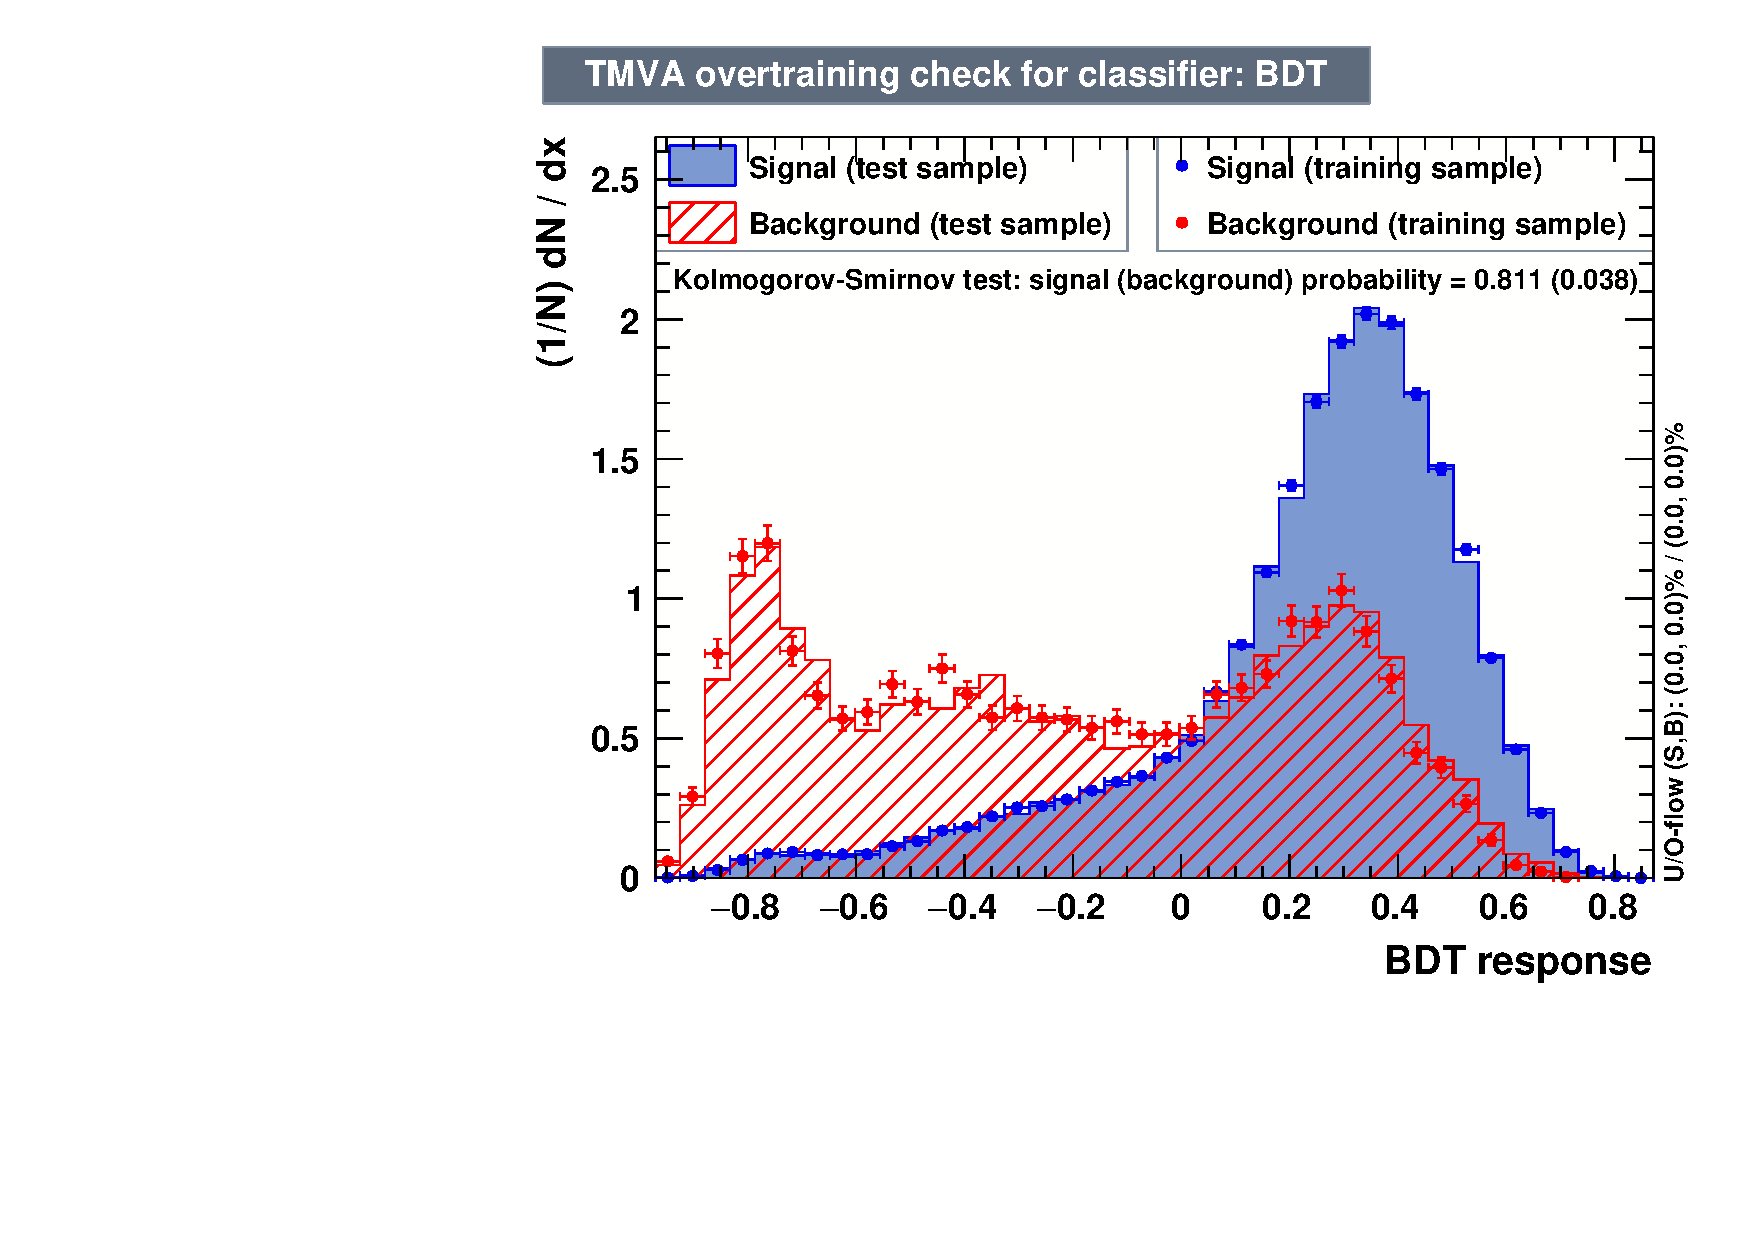
\includegraphics[width=\textwidth]{ch4_images/ks_bdt_reco}
\caption{}
\end{subfigure}
\caption{The result of a Kolmogorov-Smirnov test performed on the BDT in the truth case (a) and the reconstructed case (b).}
\label{kolmogorov smirnov bdt}
\end{figure} 


\section{Mass Bias}

Since our goal is to develop a tagger purely sensitive to the color configuration of the decaying particle, ideally our machine learning algorithms would be insensitive to the invariant mass of system. However, this is not the case.

In Figure \ref{bdt with d2} we show how different cuts on the output of the BDT depend on the invariant mass of the system in the truth case. We found that the sensitivity to the invariant mass was introduced mainly through the $D_2$ observable. Figure \ref{bdt w/o d2} shows how the dependence of the output of the invariant mass is eliminated when the BDT is trained without this observable. The same effect was found in the reconstructed case.

\begin{figure}[h]
\begin{subfigure}{1.0\textwidth}
\centering
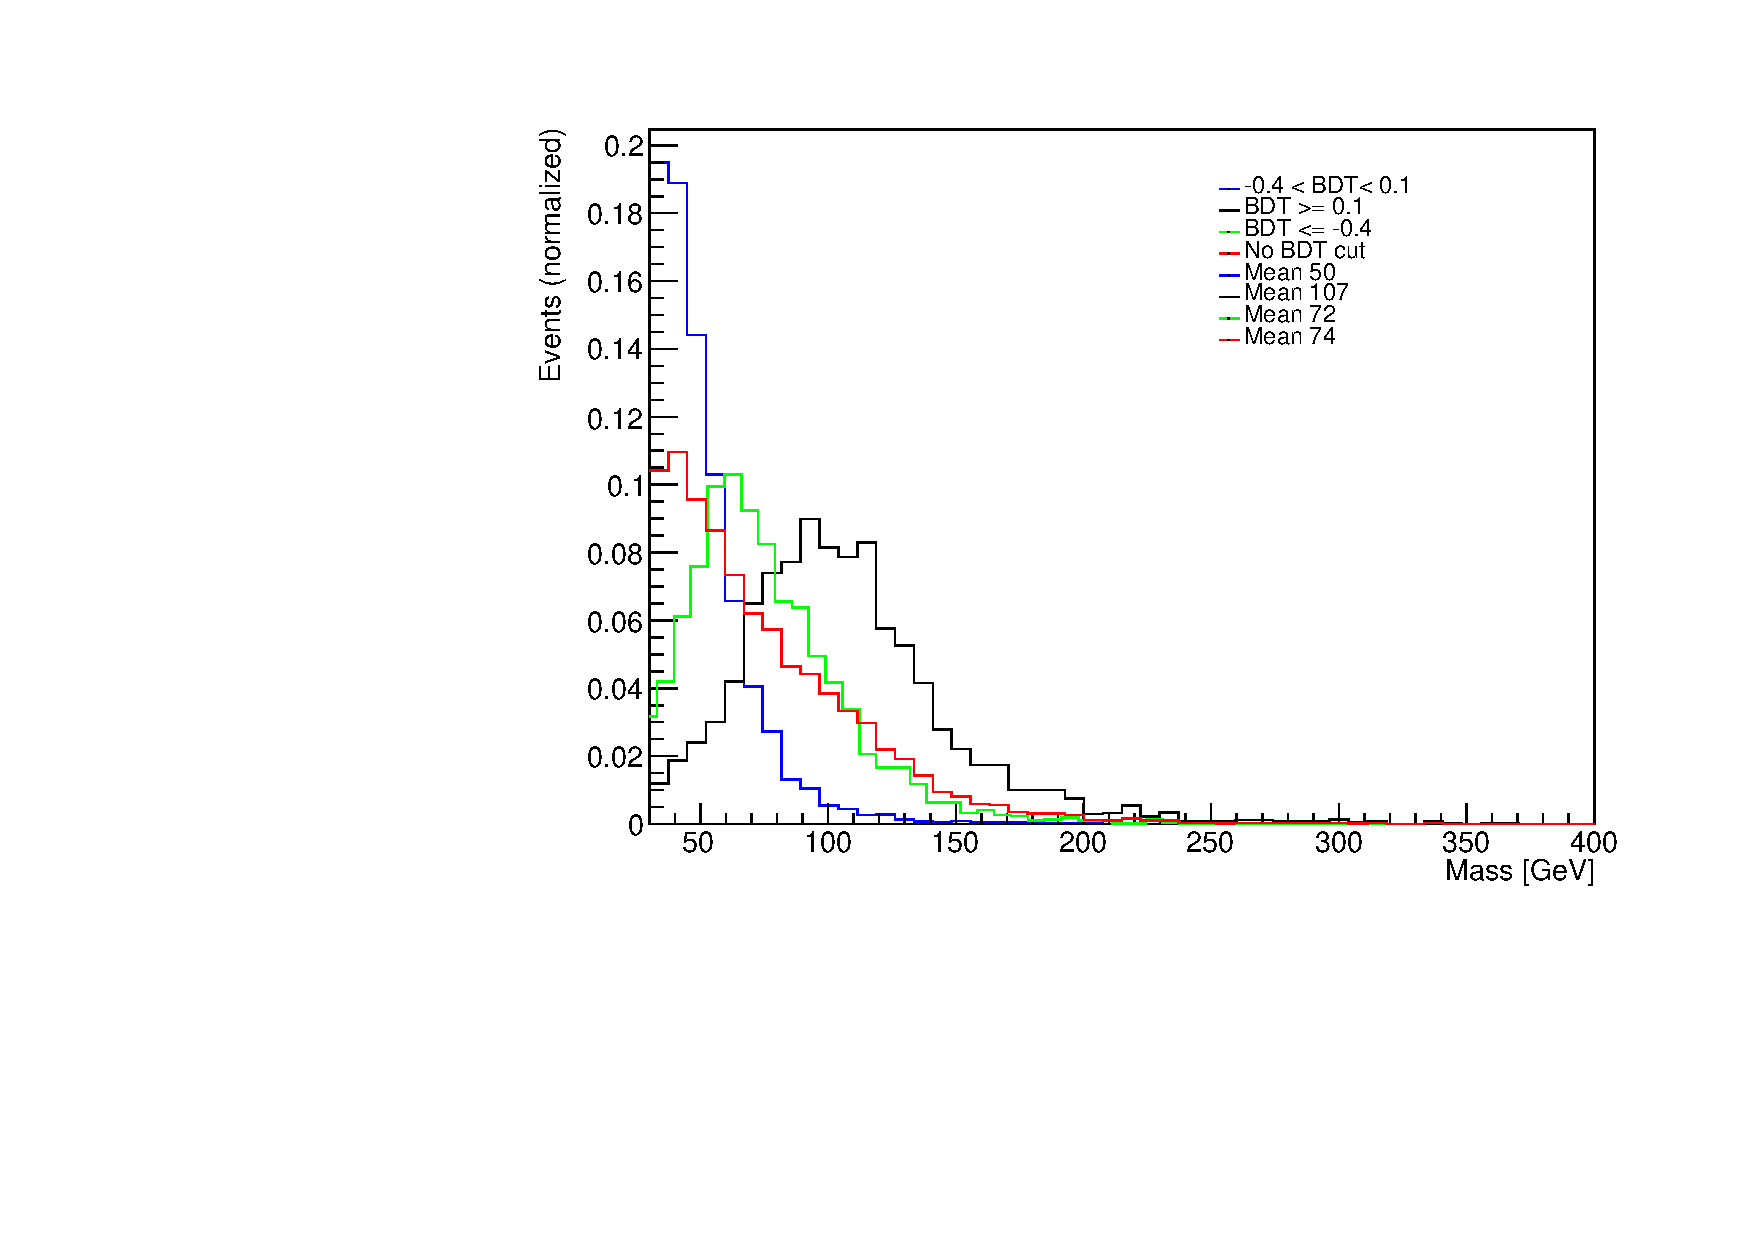
\includegraphics[width=0.9\textwidth]{ch4_images/bdt_with_d2_included}
\caption{}
\label{bdt with d2}
\end{subfigure}
\begin{subfigure}{1.0\textwidth}
\centering
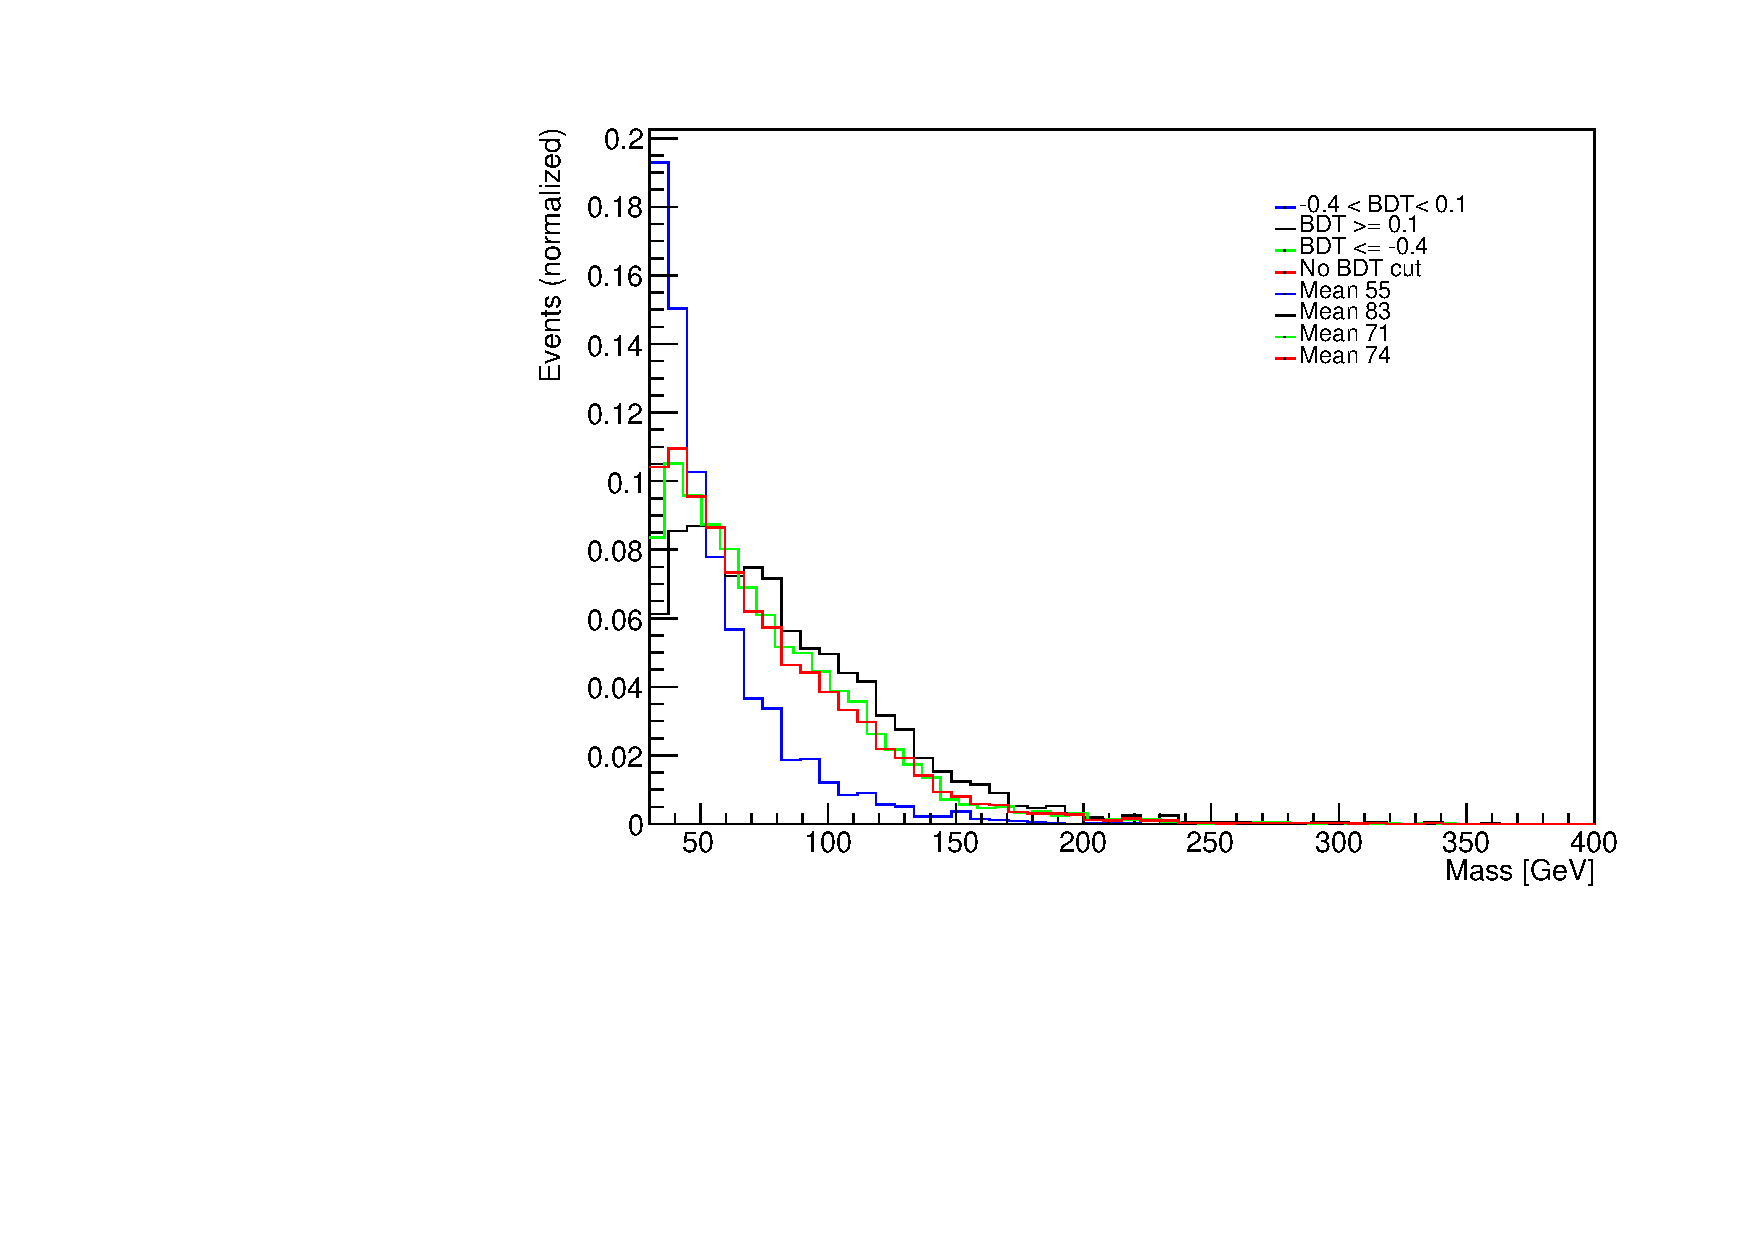
\includegraphics[width=0.9\textwidth]{ch4_images/bdt_no_d2}
\caption{}
\label{bdt w/o d2}
\end{subfigure}
\caption{The distribution of different cuts of the output of the BDT as a function of the invariant mass of the system with the inclusion of $D_2$ (a) and without the inclusion of $D_2$ (b)}
\end{figure} 

Given the fact that the $D_2$ observable is ranked as most important, the removal of this variable comes at the price of the efficiency of the algorithm. Focusing again on the truth case, Table \ref{AUC table} shows how AUCs of the MLP and BDT change when the algorithms are trained without the $D_2$ observable.

\begin{table}[h!]
\centering
\begin{tabular}{|c|c|}
\hline 
\* & AUC w/o $D_2$ \\ 
\hline 
BDT &  0.710\\ 
\hline 
MLP &  0.709\\ 
\hline 
\end{tabular}
\caption{The values of the AUC when $D_2$ is not included.}
\label{AUC table}
\end{table}

In an attempt to reduce the mass bias while still training the algorithms with $D_2$, we generated 100k new events for the signal and artificially varied the mass of the Higgs. Specifically, we generated 20k events with mass $m_H = 25$ GeV, $m_H = 50$ GeV, $m_H = 75$, $m_H = 100$ GeV and $m_H = 125$ GeV and combined them into one file. After showering these events in \code{PYTHIA8} and running the analysis, we used the output to train the machine learning algorithms. For the training, 100k background events were also generated in the same manner as described in \ref{Simulation}.

In Figure \ref{bdt inv mass} we again show how the output of the BDT depends on the invariant mass of the system. The dependence on the mass is noticeably reduced. However, with the reduction of the mass bias came a reduction of efficiency. The AUC of the BDT reduced to the values shown in Table \ref{AUC table mass bias}, despite the fact that $D_2$ was still included.

\begin{table}[h!]
\centering
\begin{tabular}{|c|c|}
\hline 
\* & AUC \\ 
\hline 
BDT & 0.651 \\ 
\hline 
MLP &  0.663\\ 
\hline 
\end{tabular}
\caption{The values of the AUC when the invariant mass of the Higgs is varied.}
\label{AUC table mass bias}
\end{table}

\begin{figure}
\centering
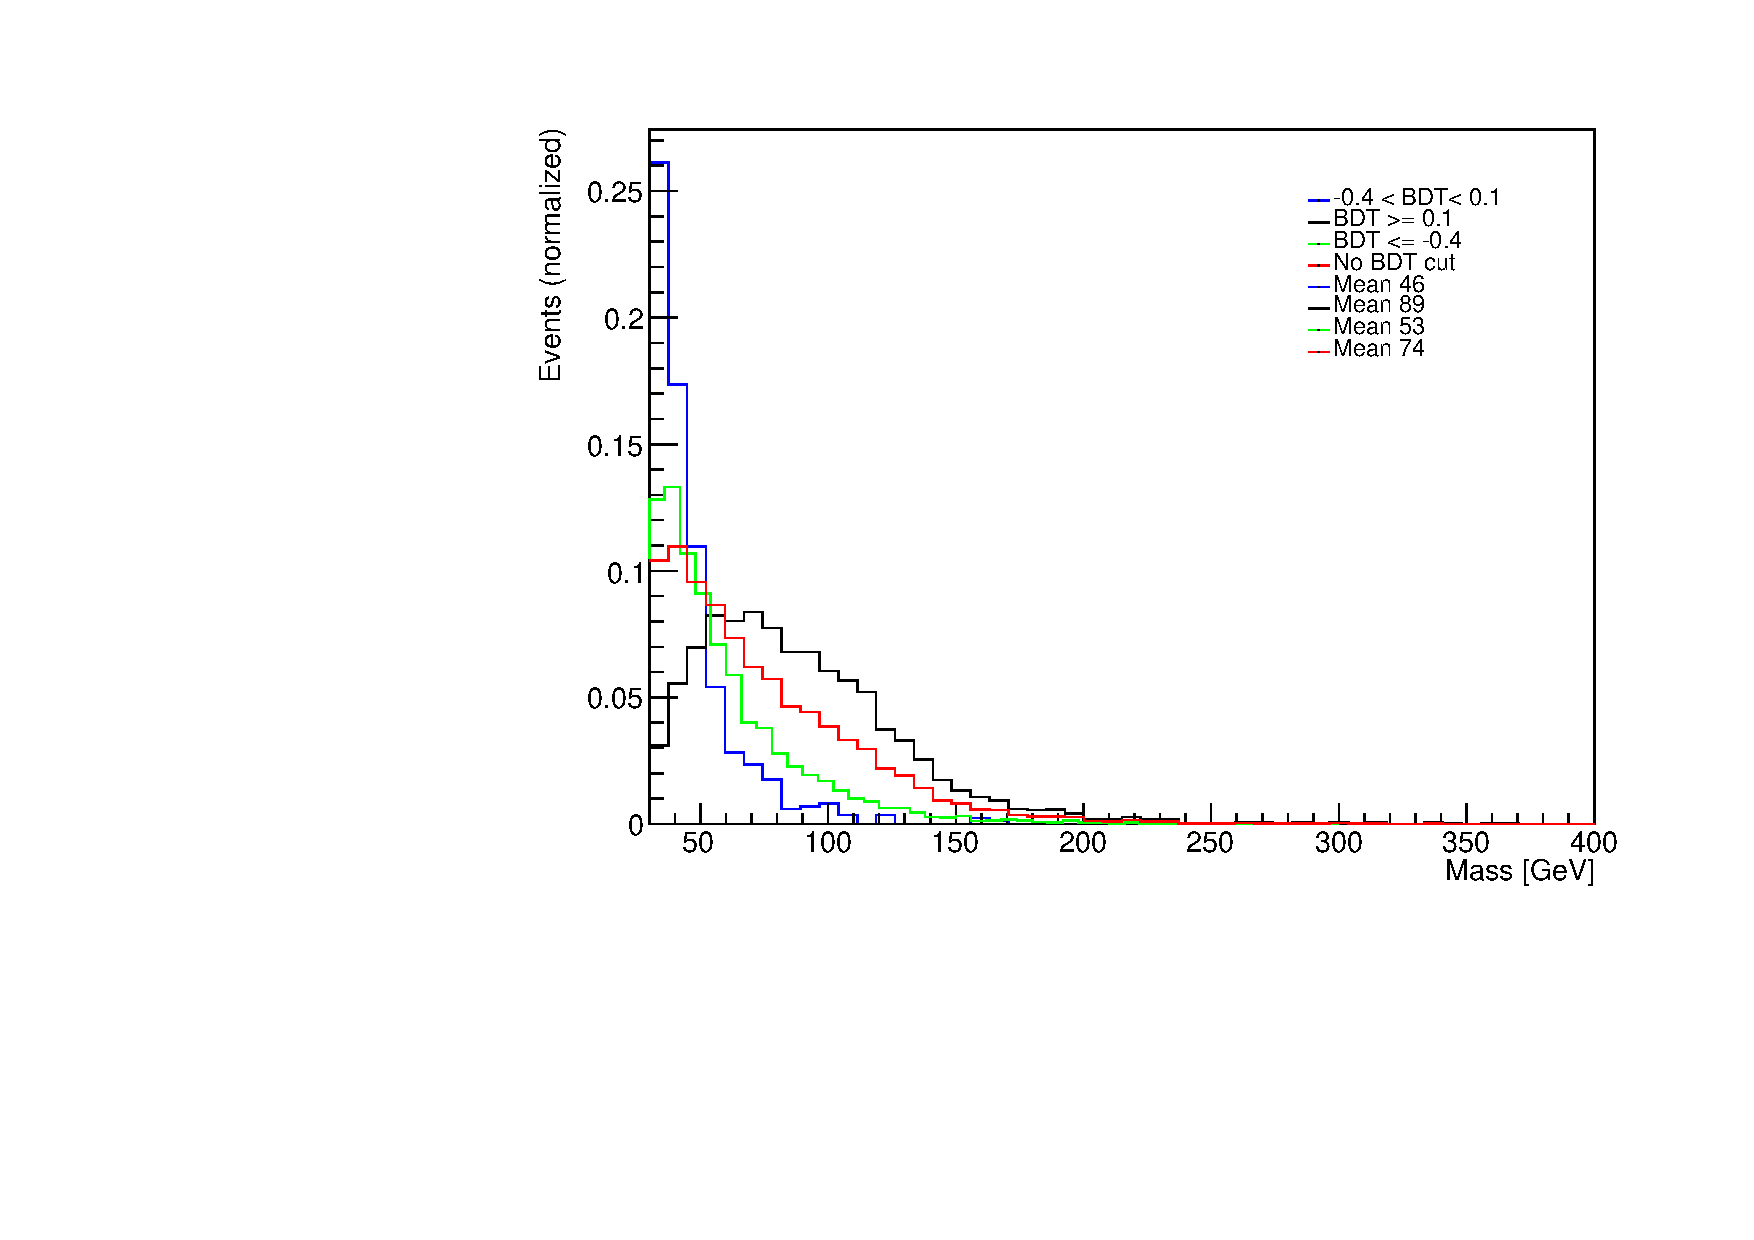
\includegraphics[scale=0.6]{ch4_images/bdt_cuts_mass_bias}
\caption{The distribution of different cuts of the output of the BDT as a function of the invariant mass of the system when this has been varied when generating hard scattering events.}
\label{bdt inv mass}
\end{figure}

We have been able to find the reason for the reduction of the AUC. Figure \ref{d2 mass bias} shows the distribution of the $D_2$ variable in the truth case when generating events with and without varying the mass of the Higgs. When the mass of the Higgs is varied, the $D_2$ distribution of the signal noticeably shifts towards that of the background. Effectively, the discrimination potential of the $D_2$ observable is reduced, explaining the reduction of the AUC.

\begin{figure}[h]
\begin{subfigure}{0.5\textwidth}
\centering
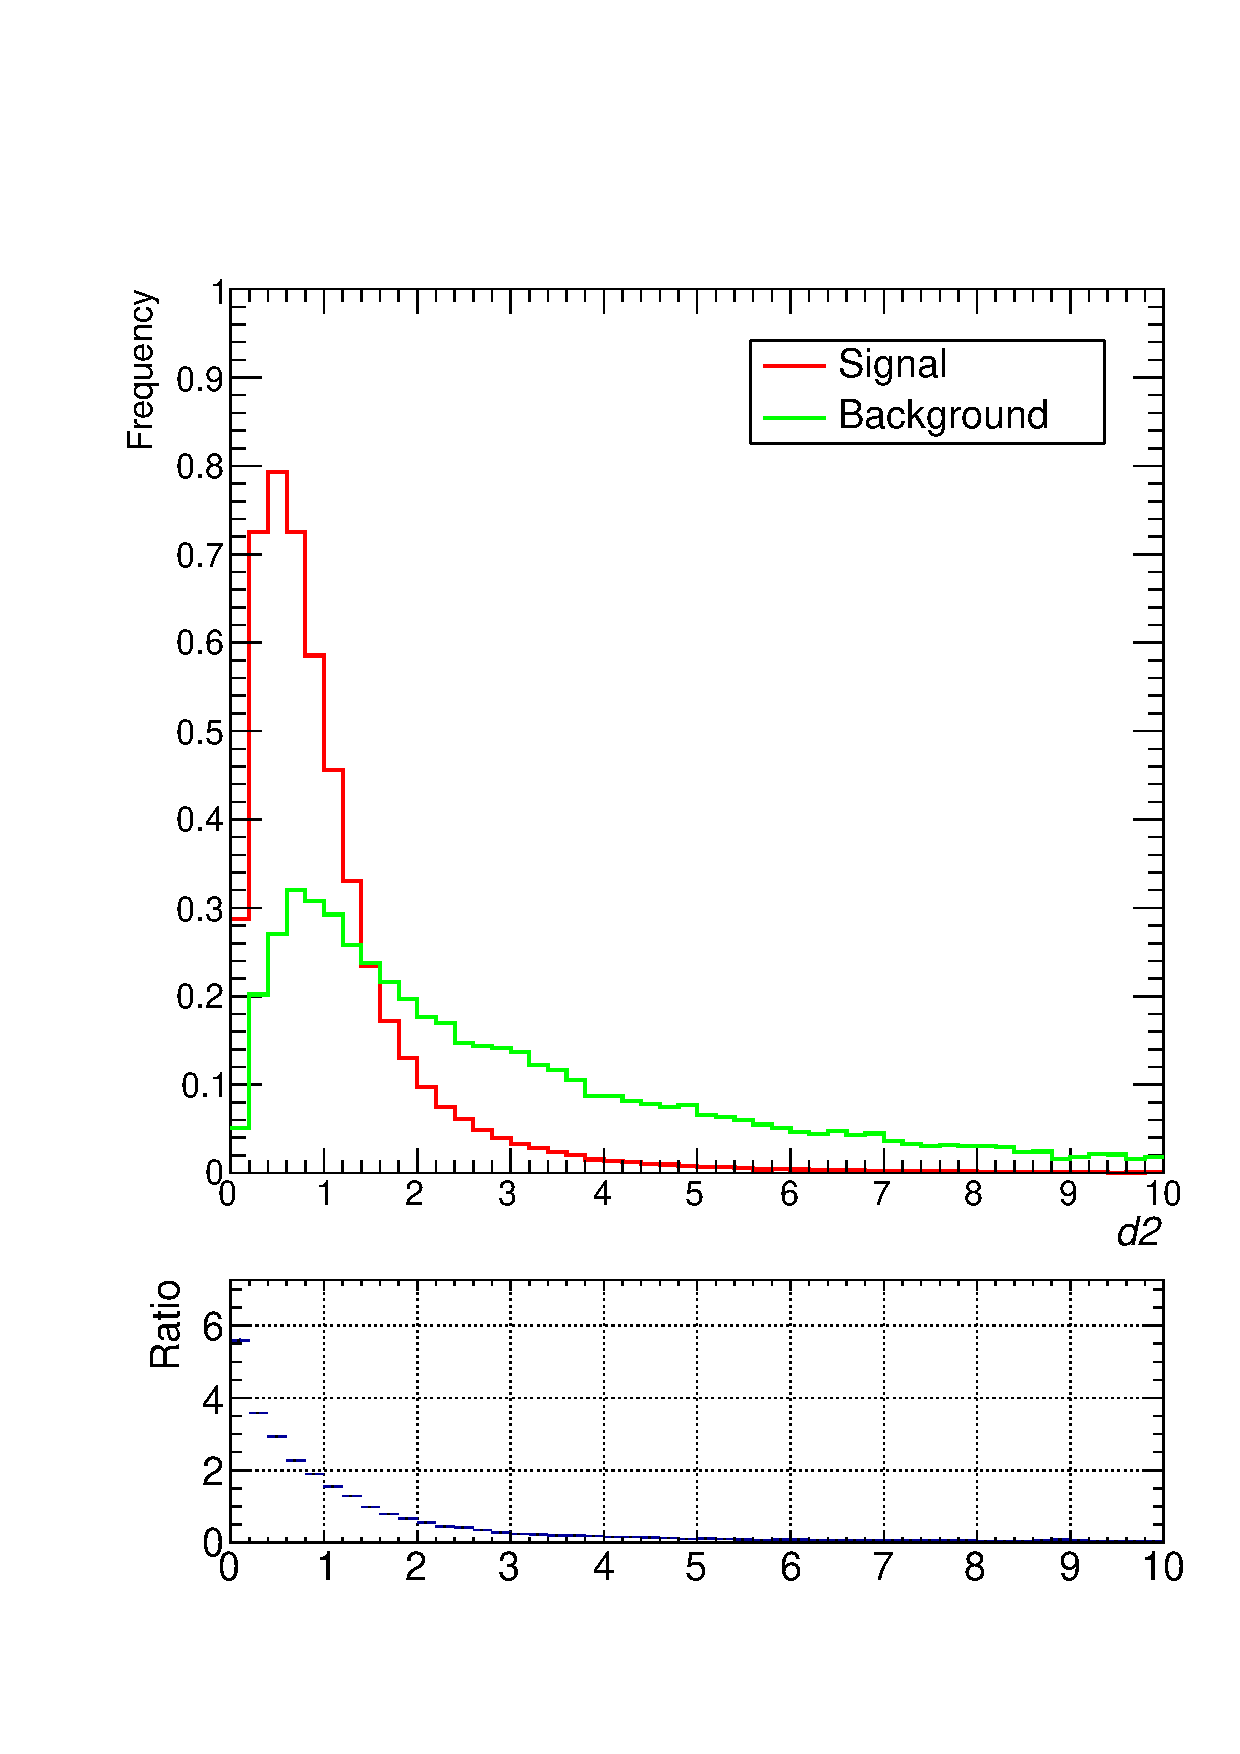
\includegraphics[scale=0.35]{ch4_images/c_d2}
\caption{}
\end{subfigure}
\begin{subfigure}{0.5\textwidth}
\centering
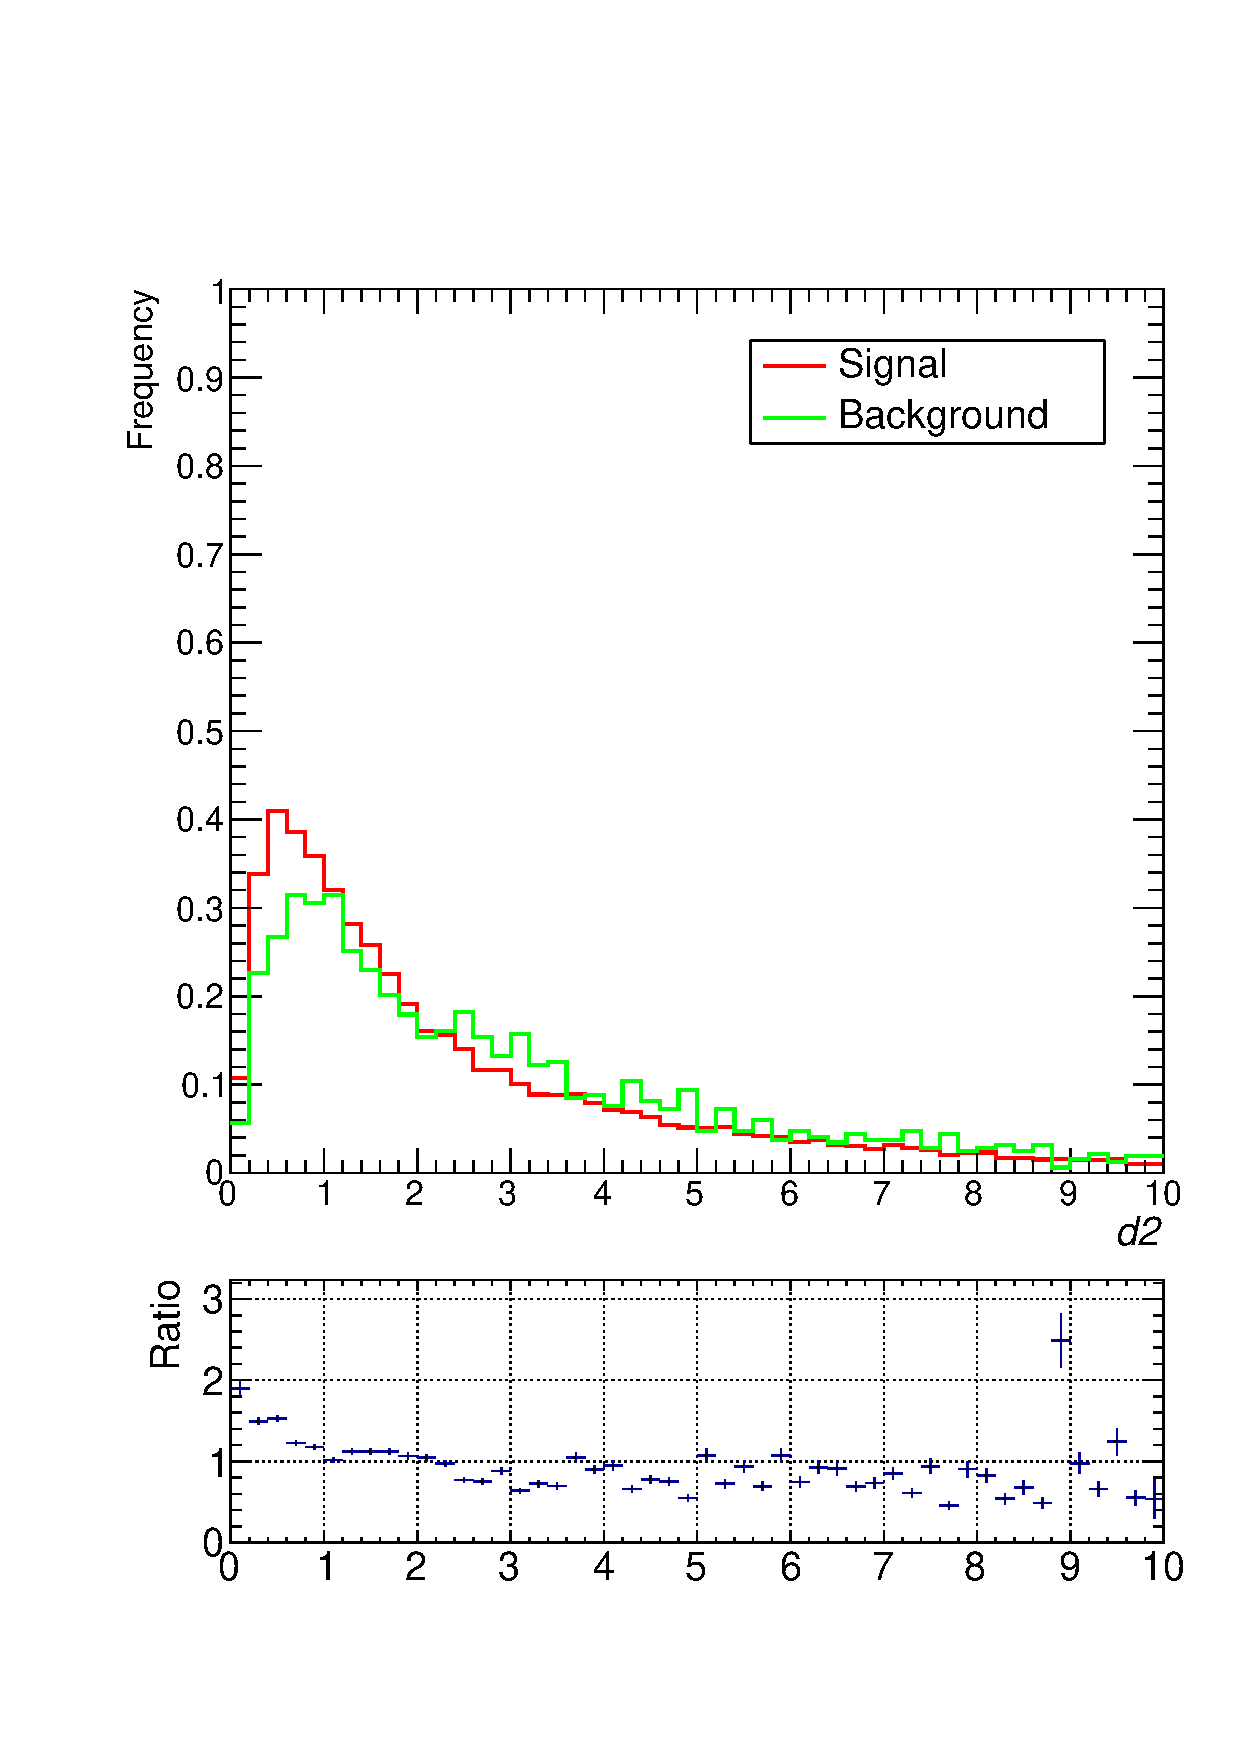
\includegraphics[scale=0.35]{ch4_images/d2_distribution_massbias}
\caption{}
\end{subfigure}
\caption{The distribution of $D_2$ before (a) and after (b) varying the mass of the Higgs.}
\label{d2 mass bias}
\end{figure}


\section{Conclusions}

Overall, we can conclude that this method for distinguishing the different color configurations of the Higgs boson and the gluon is effective both before and after the inclusion of detector effects. Unfortunately, the machine learning algorithms trained for the purpose of this classification are in part sensitive to the mass of the decaying boson. We found that the elimination of this bias comes at significant the cost of classification efficiency. In the future, we hope to find other ways to eliminate the bias, either by another machine learning approach or by debiasing a posteriori, in order to obtain a pure color tagger.

A paper summarizing the results obtained is in preparation. We are also presenting the method described above to the ATLAS Hbb working group, as the experimental community could largely profit from it.

%Descrivere la simulazione (aggiungere diagrammi di feynman)
%Descrivere l'analisi + mostrare plot (entro mercoledì)
%Machine Learning algorithms (descrivere architetture)
%Results (ROC curves)
%Further Studies - Mass debiasing, Z->bb
%Conclusion Future prospects, Lund plane, ecc. 
\end{document}